\documentclass[12pt,spanish,fleqn,openany,letterpaper,pagesize]{scrbook}

\usepackage[utf8]{inputenc}
\usepackage[spanish]{babel}%escribir con acentos sin necesidad de comandos \'{} .
\usepackage{fancyhdr}
\usepackage{epsfig}
\usepackage{epic}
\usepackage{eepic}
\usepackage{amsmath}
\usepackage{threeparttable}
\usepackage{amscd}
\usepackage{here}
\usepackage{graphicx}
\usepackage{lscape}
\usepackage{tabularx}
\usepackage{subfigure}
\usepackage{longtable}
\usepackage{multirow}
\usepackage[shortlabels]{enumitem}

\usepackage{rotating} %Para rotar texto, objetos y tablas seite. No se ve en DVI solo en PS. Seite 328 Hundebuch
                        %se usa junto con \rotate, \sidewidestable ....

\renewcommand{\theequation}{\thechapter-\arabic{equation}}
%\renewcommand{\thefigure}{\textbf{\thechapter-\arabic{figure}}}
\renewcommand{\thetable}{\textbf{\thechapter-\arabic{table}}}


\pagestyle{fancyplain}%\addtolength{\headwidth}{\marginparwidth}
\textheight22.5cm \topmargin0cm \textwidth16.5cm
\oddsidemargin0.5cm \evensidemargin-0.5cm%
\renewcommand{\chaptermark}[1]{\markboth{\thechapter\; #1}{}}
\renewcommand{\sectionmark}[1]{\markright{\thesection\; #1}}
\lhead[\fancyplain{}{\thepage}]{\fancyplain{}{\rightmark}}
\rhead[\fancyplain{}{\leftmark}]{\fancyplain{}{\thepage}}
\fancyfoot{}
\thispagestyle{fancy}%


\addtolength{\headwidth}{0cm}
\unitlength1mm %Define la unidad LE para Figuras
\mathindent0cm %Define la distancia de las formulas al texto,  fleqn las descentra
\marginparwidth0cm
\parindent0cm %Define la distancia de la primera linea de un parrafo a la margen

%Para tablas,  redefine el backschlash en tablas donde se define la posici\'{o}n del texto en las
%casillas (con \centering \raggedright o \raggedleft)
\newcommand{\PreserveBackslash}[1]{\let\temp=\\#1\let\\=\temp}
\let\PBS=\PreserveBackslash

%Espacio entre lineas
\renewcommand{\baselinestretch}{1.1}

%Neuer Befehl f\"{u}r die Tabelle Eigenschaften der Aktivkohlen
\newcommand{\arr}[1]{\raisebox{1.5ex}[0cm][0cm]{#1}}

%Neue Kommandos
\usepackage{Befehle}
%Inicio del documento. Tener en cuenta que hay archivos auxiliares

\begin{document}
\pagenumbering{roman}
%\newpage
%\setcounter{page}{1}
\begin{center}
\begin{figure}
\centering%

\epsfig{file=HojaTitulo/escudo,scale=0.6}
\end{figure}
\thispagestyle{empty} \vspace*{0cm} \textbf{\huge
Asociación de variantes en regiones codificantes de genes con datos clínicos en
pacientes colombianos usando minería de datos}\\[5.0cm]
\Large\textbf{Jennifer Vélez Segura}\\[5.0cm]
\small Universidad Nacional de Colombia\\
Facultad de Ingeniería, Departamento de Ing. Sistemas e Industrial\\
Bogotá D.C., Colombia\\
2019\\
\end{center}

\newpage{\pagestyle{empty}\cleardoublepage}

\newpage
\begin{center}
\thispagestyle{empty} \vspace*{0cm} \textbf{\huge
Asociación de variantes en regiones codificantes de genes con datos clínicos en
pacientes colombianos usando minería de datos}\\[2.0cm]
\Large\textbf{Jennifer Vélez Segura}\\[2.0cm]
\small Tesis presentada como requisito parcial para optar al
t\'{\i}tulo de:\\
\textbf{Magister en Bioinformática}\\[2.5cm]
Director(a):\\
Ph.D. Elizabeth León Guzmán\\[2.0cm]
L\'{\i}nea de Investigaci\'{o}n:\\
Minería de datos en Bioinformática\\
Grupo de Investigaci\'{o}n:\\
MIDAS\\[2.5cm]
Universidad Nacional de Colombia\\
Facultad Ingeniería, Departamento de Ing. Sistemas e Industrial\\
Bogotá D.C., Colombia\\
2019 \\
\end{center}

\newpage{\pagestyle{empty}\cleardoublepage}

\newpage
\thispagestyle{empty} \textbf{}\normalsize
\\\\\\%
\textbf{(Dedicatoria)}\\[4.0cm]

\begin{flushright}
\begin{minipage}{8cm}
    \noindent
        Esta tesis esta dedicada a mi familia quienes han sido mi principal apoyo y soporte durante toda mi vida y a mi mejor amiga que en paz descanse Camila Marcela Sanchez Rubio.\\[1.0cm]\\
      \end{minipage}
\end{flushright}

\newpage{\pagestyle{empty}\cleardoublepage}

\newpage
\thispagestyle{empty} \textbf{}\normalsize
\\\\\\%
\textbf{\LARGE Agradecimientos}
\addcontentsline{toc}{chapter}{\numberline{}Agradecimientos}\\\\
A mis amigos Sergio Solano y Julián Cruz quienes me apoyaron, durante todo el proceso de desarrollo del trabajo, al laboratorio Genetix S.A.S quienes donaron la información utilizada en el presente trabajo, a mis compañeras del laboratorio,a mi familia por todo el apoyo y la paciencia.Finalmente a la profesora Elizabeth León Gúzman por la aceptar la dirección del trabajo y prestar todos sus conocimientos para la culminación de este trabajo. \\

\newpage{\pagestyle{empty}\cleardoublepage}

\newpage
\textbf{\LARGE Resumen}
\addcontentsline{toc}{chapter}{\numberline{}Resumen}\\\\
Se realizo una implementación y validación de un pipeline para la idententifiación de variantes a partir de 4813 secuenciados. Se diseño e implemento un modelo de datos para la gestión de la información de las variantes obtenidas y se le adiciono la información clínica disponible para 227 pacientes. Se diseño un modelo de minería de datos basados en procesamiento de lenguaje natural de las historias clínicas y las cuales se les realizo un agrupamiento, una vez obtnidos los grupos se aplicaron reglas de asociación por cada uno de los grupos obtenidos y por dos genes que fueron el CFTR y RB1. Los resultados obtenidos fueron variantes prefiltradas por calidad, una base de datos implementada con la información clínica y las variantes y finalmente se obtuvieron 5 grupos de pacientes con sus reglas de asociación y una caracterización de variantes en CFTR y RB1 en toda la base de datos. Se implemento un modelo de minería que permite caracterizar y asociar la frecuencia de variantes en genes a las características clínicas de los pacientes. \\

\textbf{\small Palabras clave: Secuenciación, variantes, región codificante, minería de datos, clustering, reglas de asociación, sistemas de información, características clíncias}.\\


\textbf{\LARGE Abstract}\\\\
Es el mismo resumen pero traducido al ingl\'{e}s. Se debe usar una extensi\'{o}n m\'{a}xima de 12 renglones. Al final del Abstract se deben traducir las anteriores palabras claves tomadas del texto (m\'{\i}nimo 3 y m\'{a}ximo 7 palabras), llamadas keywords. Es posible incluir el resumen en otro idioma diferente al espa\~{n}ol o al ingl\'{e}s, si se considera como importante dentro del tema tratado en la investigaci\'{o}n, por ejemplo: un trabajo dedicado a problemas ling\"{u}\'{\i}sticos del mandar\'{\i}n seguramente estar\'{\i}a mejor con un resumen en mandar\'{\i}n.\\[2.0cm]
\textbf{\small Keywords: palabras clave en ingl\'{e}s(m\'{a}ximo 10 palabras, preferiblemente seleccionadas de las listas internacionales que permitan el indizado cruzado)}\\


\renewcommand{\tablename}{\textbf{Tabla}}
\renewcommand{\figurename}{\textbf{Figura}}
\renewcommand{\listtablename}{Lista de Tablas}
\renewcommand{\listfigurename}{Lista de Figuras}
\renewcommand{\contentsname}{Contenido}
\tableofcontents % indice de tablas


%\newcommand{\clearemptydoublepage}{\newpage{\pagestyle{empty}\cleardoublepage}}

%\chapter*{Lista de s\'{\i}mbolos}
\addcontentsline{toc}{chapter}{\numberline{}Lista de s\'{\i}mbolos}
Esta secci\'{o}n es opcional, dado que existen disciplinas que no manejan s\'{\i}mbolos y/o abreviaturas.\\

Se incluyen s\'{\i}mbolos generales (con letras latinas y griegas), sub\'{\i}ndices, super\'{\i}ndices y abreviaturas (incluir s\'{o}lo las clases de s\'{\i}mbolos que se utilicen). Cada una de estas listas debe estar ubicada en orden alfab\'{e}tico de acuerdo con la primera letra del s\'{\i}mbolo.
\section*{S\'{\i}mbolos con letras latinas}
 \label{simbolos}
 \renewcommand{\arraystretch}{1.3}
%\begin{longtable}[l]{*{4}{>{$}l<{$}}p{9cm}}
\begin{longtable}[l]{>{$}l<{$}l>{$}l<{$}>{$}l<{$}}
%\begin{tabular}
\textbf{S\'{\i}mbolo}&\textbf{T\'{e}rmino}&\textbf{Unidad SI}&\textbf{Definici\'{o}n}\\[0.5ex]\hline
\endfirsthead%
\textbf{S\'{\i}mbolo}&\textbf{T\'{e}rmino}&\textbf{Unidad SI}&\textbf{Definici\'{o}n}\\[0.5ex]\hline
\endhead%
      A              &\'{A}rea                                   &\text{m}^{2}                         &\int\int dxdy\\%
      A_{\text{BET}} &\'{A}rea interna del s\'{o}lido                &\frac{\text{m}^{2}}{\text{g}}        &\text{ver DIN ISO 9277}\\%
      A_{\text{g}}   &\'{A}rea transversal de la fase gaseosa    &\text{m}^{2}                         &\text{Ec...}\\%
      A_{\text{s}}   &\'{A}rea transversal de la carga a granel  &\text{m}^{2}                         &\text{Ec...}\\%
      a              &Coeficiente                            &1                                    &\text{Ec...}\\%
      a              &Contenido de ceniza                    &1                                    &\frac{m_{\text{ceniza}}}{m_{\text{bm,0}}}\\%
      c              &Contenido de carbono                   &1                                    &\frac{m_{\text{C}}}{m}\\%
      c              &Longitud de la cuerda                  &\text{m}                             &\text{Figura...}\\
      c              &Concentraci\'{o}n de la cantidad de materia&\frac{\text{mol}}{\text{m}^{3}}      &\frac{n}{V}\\%
      D              &Di\'{a}metro                               &\text{m}                             &\\%
      E_{\text{A}}   &Energ\'{\i}a de activaci\'{o}n                  &\frac{\text{kJ}}{\text{mol}}         &\text{Ec....}\\%
      F              &Fracci\'{o}n de materia vol\'{a}til            &1                                    &\text{ver DIN 51720}\\%
      Fr             &N\'{u}mero de Froude                       &1                                    &\frac{\omega^{2}R}{g_{\text{0}}}\\%
      \overrightarrow{g}&Aceleraci\'{o}n de la gravedad          &\frac{\text{m}}{\text{s}^{2}}        &\frac{d^{2}\overrightarrow{r}}{dt^{2}}\\%
      H              &Entalp\'{\i}a                               &\text{J}                             &U+PV\\%
      H_{\text{o}}   &Poder calor\'{\i}fico superior              &\frac{\text{MJ}}{\text{kg}}          &\text{ver DIN 51857}\\%
      h              &Contenido de hidr\'{o}geno                 &1                                    &\frac{m_{\text{H}}}{m}\\%
      K              &Coeficiente de equilibrio              &1                                    &\text{Ec...}\\%
      L              &Longitud                               &\text{m}                             &DF\\%
      L              &Longitud del reactor                   &\text{m}                             &\text{Figura...}\\%
      m              &Masa                                   &\text{kg}                            &DF\\%
      \dot{m}        &Flujo de masa                          &\frac{\text{kg}}{\text{s}}           &\frac{m}{t}\\%
      n              &Velocidad de rotaci\'{o}n                  &\frac{\text{1}}{\text{s}}            &\frac{\omega}{2\pi}\\%
      n              &Cantidad de materia                    &\text{mol}                           &DF\\%
      P              &Presi\'{o}n                                &\text{Pa}                            &\frac{\vec{F}\cdot\vec{n}}{A}\\%
      Q              &Calor                                  &\text{kJ}                            &\text{1. $LT$}\\%
      T              &Temperatura                            &\text{K}                             &DF\\%
      t              &Tiempo                                 &\text{s}                             &DF\\%
      x_{\text{i}}   &Fracci\'{o}n de la cantidad de materia     &1                                    &\frac{n_{\text{i}}}{n}\\%
      V              &Volumen                                &\text{m}^{3}                         &\int{dr^{3}}\\%
      \vec{u}        &Velocidad                              &\frac{\text{m}}{\text{s}}            &(\frac{dr}{dt},r\frac{d\upsilon}{dt},\frac{dz}{dt})\\%
      w_{\text{i}}   &Fracci\'{o}n en masa del componente i      &1                                    &\frac{m_{\text{i}}}{m_{\text{0}}}\\%
      w_{\text{w,i}} &Contenido de humedad de la sustancia i &1                                    &\frac{m_{\text{\wasser}}}{m_{\text{i,0}}}\\%
      Z              &Factor de gases reales                 &1                                    &\frac{pv}{RT}\\%
\end{longtable}
\vspace{5ex}
\section*{S\'{\i}mbolos con letras griegas}

\begin{longtable}[l]{>{$}l<{$}l>{$}l<{$}>{$}l<{$}}
\textbf{S\'{\i}mbolo}&\textbf{T\'{e}rmino}&\textbf{Unidad SI}&\textbf{Definici\'{o}n}\\[0.5ex] \hline%
\endfirsthead%
\textbf{S\'{\i}mbolo}&\textbf{T\'{e}rmino}&\textbf{Unidad SI}&\textbf{Definici\'{o}n}\\[0.5ex] \hline%
\endhead%
\renewcommand{\arraystretch}{1.3}
 \label{simbolosg}
     \alpha_{\text{BET}}  &Factor de superficie                  &\frac{\text{m}^{2}}{\text{g}}   &(w_{\text{F,waf}})(A_{\text{BET}})\\%
     \beta_{\text{i}}     &Grado de formaci\'{o}n del componente i   &1                               &\frac{m_{\text{i}}}{m_{\text{bm,0}}}\\%
     \gamma               &Wandhaftreibwinkel (Stahlblech)       &1                               &\text{Secci\'{o}n...}\\
     \epsilon             &Porosidad de la part\'{\i}cula             &1                               &1-\frac{\rho_{\text{s}}}{\rho_{\text{w}}}\\%
     \eta                 &mittlere Bettneigungswinkel (St\"{u}rzen) &1                               &\text{Figura...}\\%
     \theta               &\'{A}ngulo de inclinaci\'{o}n de la cama      &1                               &\text{Figura...}\\
     \theta_{\text{O}}    &\'{A}ngulo superior de avalancha          &1                               &\text{Figura...}\\
     \theta_{\text{U}}    &\'{A}ngulo inferior de avalancha          &1                               &\text{Figura...}\\
     \kappa               &Velocidad de calentamientoe           &\frac{\text{K}}{\text{s}}       &\frac{dT}{dt}\\%
     \nu                  &Coeficiente estequiom\'{e}trico           &1                               &\text{ver DIN 13345}\\%
     \rho_{\text{b}}      &Densidad a granel                     &\frac{\text{kg}}{\text{m}^{3}}  &\frac{m_{\text{S}}}{V_{\text{S}}}\;(\text{Secci\'{o}n...})\\
     \rho_{\text{s}}      &Densidad aparente                     &\frac{\text{kg}}{\text{m}^{3}}  &\frac{m_{\text{F}}}{V_{\text{P}}}\;(\text{Secci\'{o}n...})\\
     \rho_{\text{w}}      &Densidad verdadera                    &\frac{\text{kg}}{\text{m}^{3}}  &\frac{m_{\text{F}}}{V_{\text{F}}}\;(\text{Secci\'{o}n...})\\
     \tau                 &Tiempo adimensional                   &1                               &\text{Ec....}\\%
     \Phi_{\text{V}}      &Flujo volum\'{e}trico                     &\frac{\text{m}^{3}}{\text{s}}   &\frac{\Delta V}{\Delta t}\\
     \omega               &Velocidad angular                     &\frac{1}{\text{s}}              &\frac{d\upsilon}{dt}\\

\end{longtable}


\section*{Sub\'{\i}ndices}
\begin{longtable}[l]{>{}l<{}l}
  \textbf{Sub\'{\i}ndice} & \textbf{T\'{e}rmino} \\[0.5ex] \hline%
  \endfirsthead%
  \textbf{Sub\'{\i}ndice} & \textbf{T\'{e}rmino} \\[0.5ex] \hline%
  \endhead%
\renewcommand{\arraystretch}{1.4}\label{simbolosg}

 bm&materia org\'{a}nica\\%
 DR&Dubinin-Radushkevich\\%
 E&Experimental\\%
 g&Fase gaseosa\\%
 k&Condensado\\%
 Ma&Macroporos\\%
 P&Part\'{\i}cula\\%
 p&Poro\\%
 p&Pirolizado\\%
 R&Reacci\'{o}n\\%
 t&Total\\%
 wf&Libre de agua\\%
 waf&Libre de agua y de ceniza\\%
 0&Estado de referencia\\%

\end{longtable}


\setlength{\extrarowheight}{0pt}


\section*{Super\'{\i}ndices}
\begin{longtable}[l]{>{}l<{}l}
  \textbf{Super\'{\i}ndice} & \textbf{T\'{e}rmino} \\[0.5ex] \hline%
  \endfirsthead%
  \textbf{Super\'{\i}ndice} & \textbf{T\'{e}rmino} \\[0.5ex] \hline%
  \endhead%
\renewcommand{\arraystretch}{1.4}\label{simbolosg}

 n &Coeficiente x\\%



\end{longtable}


\setlength{\extrarowheight}{0pt}


\section*{Abreviaturas}
\begin{longtable}[l]{>{}l<{}l}
  \textbf{Abreviatura} & \textbf{T\'{e}rmino} \\[0.5ex] \hline%
  \endfirsthead%
  \textbf{Abreviatura} & \textbf{T\'{e}rmino} \\[0.5ex] \hline%
  \endhead%
\renewcommand{\arraystretch}{1.4}\label{simbolosg}
 1.$LT$&Primera ley de la termodin\'{a}mica\\%
 $DF$    &Dimensi\'{o}n fundamental\\%
 $RFF$   &Racimos de fruta fresca\\%

\end{longtable}


\setlength{\extrarowheight}{0pt}
%\include{Resumen}%\newcommand{\clearemptydoublepage}{\newpage{\pagestyle{empty}\cleardoublepage}}
\pagenumbering{arabic}
\cleardoublepage
\addcontentsline{toc}{chapter}{Lista de figuras} % para que aparezca en el indice de contenidos
\listoffigures % indice de figuras

\cleardoublepage
\addcontentsline{toc}{chapter}{Lista de tablas} % para que aparezca en el indice de contenidos
\listoftables % indice de tablas

\chapter{Estado del Arte}

Con el desarrollo de la las tecnologías de secuenciación masiva los biólogos moleculares se han visto en la necesidad  de utilizar metodologías computacionales para analizar datos biológicos a gran escala, además de la aplicación de estas tecnologías en medicina requieren de una estandarización y diseño que permita obtener nuevos conocimientos que sean  aplicables en la salud de los colombianos.

\section{Biología molecular y secuenciación masiva.}

Desde  que  Watson y Crick propusieron la estructura del ADN en 1953 \cite{Watson1953}, el estudio del ADN ha sido básico en el desarrollo de la biología molecular, incluso el mismo Francis Crick fue quien propuso el dogma central de la misma para describir la relevancia del ADN en los seres vivos y la utilización de la información que contiene por las células,dada la importancia del  ADN  en las décadas de 1970 y 1980 se desarrollaron  técnicas para determinar el orden de los nucleótidos  (técnicas de secuenciación) de manera más eficiente que la secuenciación de las proteínas y se definieron secuencias de algunos organismos como el virus de Episten Barr y  de la mitocondria humana, mediante la utilización de métodos químicos propuestos por Maxam y Gilbert en 1977 y Sanger en 1980 siendo este último el más popular, estas técnicas son conocidas como tecnicas primera generación \cite{Herraez2012}. \\

Dada la importancia del  ADN  en las décadas de 1970 y 1980 se desarrollaron  técnicas para determinar el orden de los nucleótidos  (técnicas de secuenciación) de una manera más eficiente que la secuenciación de las proteínas y se definieron secuencias de algunos organismos como el virus de Episten Barr y  de la mitocondria humana, mediante la utilización de métodos químicos propuestos por Maxam y Gilbert en 1977 y Sanger en 1980 siendo este último el más popular, estas técnicas son conocidas como técnicas primera generación \cite{Herraez2012}. \\

Los métodos desarrollados para secuenciar prosperaron y con el proyecto del genoma humano que comenzó en 1980 y fue completado en el 2003, permitió que se desarrollaran nuevas tecnologías para optimizar el proceso de secuenciación y disminuir sus costos, inicialmente fue el secuenciador de Illumina  que en el 2008 permitió obtener el primer individuo humano secuenciado con esta tecnología \cite{Pei}. Estas nuevas tecnologías se fueron desarrollando en otras plataformas, tales como el secuenciador de roche 454 y el SOLiD de applied biosisten \cite{Pei} y son conocidas como tecnologías de última generación o de siguiente generación (Next-generation sequencing, NGS), que tienen la capacidad de realizar secuenciaciones de alto rendimiento de una maneras más rápida y económica que las de primera generación \cite{Herraez2012}. La diferencia entre las técnicas de secuenciación de primera generación y las de NGS se presenta en el hecho de que la nueva generación genera lecturas de menos de 500 pares de bases en comparación a las 1000 pares de bases de sanger \cite{Pei,Kulski2016}. \\
 
El desarrollo de estas tecnologías ha hecho que los datos genómicos aumenten de una manera vertiginosa, y permiten que se pueda realizar análisis en diferentes organismos con aplicaciones en biotecnología y salud \cite{Herraez2012}. Se ha estimado que cada genoma humano tiene alrededor de 3.5 millones de diferencias con respeto al genoma de referencia (Genoma de consenso para la salud humana), estas diferencias son llamadas variantes y pueden determinan el fenotipo de los individuos, algunas de estas variantes son conocidas para indicar predisposiciones a enfermedades \cite{Kutzera2017}.\\

En el campo de la salud actualmente se emplea la secuenciación de exomas es la más utilizada puesto que se considera que los exones son las regiones de ADN conservadas y expresadas, (se traducirán en ARNm y posteriormente en proteínas) y representan menos del 2\% el genoma humano pero se estima que contiene el 85\% de las variantes conocidas de enfermedades, lo que permite la reducción de costos y una buena alternativa frente a la secuenciación de genomas completos \cite{Illumina2017,Klug2013,Herraez2012}.\\

Dado que la utilización de NGS permitío dar respuesta para entender enfermedades raras, ya que fue posible identificar las regiones responsables de una enfermedad, teniendo como control los datos poblacionales como el proyecto de 1000 genomas, los datos genómicos pueden también pueden ser útiles para la caracterización de enfermedades poligénicas y su asociación con las variaciones genómicas presentes en el individuo \cite{Poliakov2015}.\\

La secuenciación de exones (secuenciación de exoma) ha sido un buen método para identificar SNPs (Polimorfismos de Nucleótido Único) y los SNV (Variantes de nucleótido simple) como se observa en la sigueinte figura \ref{fig:snp}, y permitió identificar pequeñas delecciones o inserciones (indels) que pueden  ser la causa de enfermedades y de la variación en los fenotipos \cite{Deng2011,Wenger2017}.\\

\begin{figure}[H] 
	\centering
	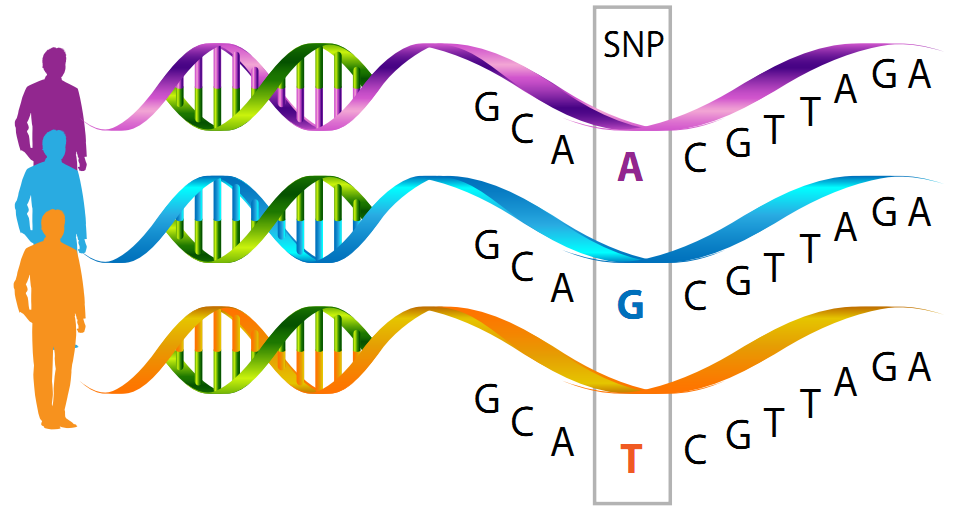
\includegraphics[width=0.8\textwidth]{Estado/snp}
	\caption{SNPs en Humanos.} \label{fig:snp}
\end{figure} 

A partir de la información pública disponible se ha estimado que las variantes pueden afectar la función de la proteína ya su vez pueden estar asociados a otros genes dentro de una enfermedad, aunque en genética humana la frecuencia de una variante especifica dentro de la población es clasificada como benigna (No genera una enfermedad), por ello la importancia de la integración de la información y la revisión de la variante \cite{Shendure2016}.\\

La identificación de variantes se realiza con diversas plataformas siendo el MiSeq es un sistema de secuenciación de illumina que permite la secuenciación de 4800 genes en un solo experimento y una de las más populares \cite{Illumina2017}. En cuanto al análisis de los datos esta plataforma incluye un servicio de computación en la nube (BaseSpace), donde los datos biológicos son analizados  sin necesidad de que los investigadores tengan habilidades en bioinformática. Pero están disponibles como herramientas solamente de investigación y no como diagnóstico {\cite{Illumina2017}. \\

A pesar de ser herramientas de investigación  que han sido desarrolladas, Illumina permite que dentro del BaseSpace se publiquen nuevos algoritmos, herramientas abiertas o aplicaciones diseñadas por desarrolladores que permitan mejorar estos análisis genómicos y  la aplicación en diversas en sus diversas plataformas de secuenciación que ofrece esta empresa \cite{Illumina2017}. \\

Los datos obtenidos a partir de técnicas de NGS han tenido un crecimiento vertiginoso y presentan un reto para el manejo y análisis de los mismos, debido a que los formatos de los datos y las inconsistencias de las secuencias como resultado de los procesos experimentales, la importación de las secuencias a nivel digital, el ensamble de los fragmentos de ADN, el alineamiento y post-alineamiento de grandes cantidades de datos biológicos hace que se convierta en una de las bases de la investigación en bioinformática \cite{Deng2011,Triplet2014}.\\

\subsection{La secuenciación de siguiente generación (NGS) aplicaciones en salud}

La secuenciación de siguiente generación ha sido adoptada en el ambito clínico, dado que se ha documentado su utilidad para el diagnostico de enfermedades  y para la toma de decisiones en cáncer o para la selección de dosis de medicamentos en un paciente, \cite{Lubin2017} algunos de estos ejemplos son:

\subsubsection*{Cáncer de Seno}

El cáncer de seno es una enfermedad que afecta principalmente a mujeres y que en estadios avanzados tienen una alta tasa de mortalidad por lo que ha recibido una importante atención de por la comunidad de investigadores, principalmente en el área biomédica con la intención de buscar marcadores genéticos de la enfermedad. Actualmente se encuentra una gran cantidad de investigaciones publicadas, donde se intenta visualizar las interacciones de los genes como esos marcadores en las distintas poblaciones \cite{Jurca2016}.\\

Teniendo en cuenta que el cáncer el resultado de una mutación de ADN, donde la consecuencia es que la célula portadora de la mutación pierda su funcion normal y gane la habilidad de multiplicarse de manera indefinida sobre los tejidos normales. Donde la identificación más común para realizar la identificación de biomarcadores geneticos es la utilización de NGS, donde la variación de un gen puede alterar la función celular y se causal de la enfermedad y en algunos casos puede ser heredable y predisponente al desarrollo de la enfermedad \cite{Jurca2016,Wenger2017}.


\subsubsection*{Fibrosis Quistica}

La fibrosis quística es una enfermedad multisistemica causada por mutaciones puntuales en el gen CFTR, las características típicas de esta enfermedad son: la enfermedad pulmonar obstructiva, infecciones bacterianas crónicas de las vías respiratorias y senos paranasales e infertilidad masculina debida  a azoospermia obstructiva, la mayoría de los pacientes con esta enfermedad tienen insuficiencia pancreática, es frecuente que los pacientes con fibrosis quistica tengan mutaciones en el gen CFTR con un efecto funcional de la proteína leve, se han identificado 2000 variantes asociados a esta enfermedad \cite{Terlizzi2017}. 


\section{Bioinformática}

La bioinformática trata sobre el almacenamiento, simulación y análisis de datos biológicos con el uso de herramientas computacionales como la minería de datos, siendo definida como una herramienta de investigación, desarrollo y aplicación de enfoques computacionales para expandir el uso de los datos biológicos y médicos, incluyendo las herramientas que permitan almacenar, archivar y análisis o visualizar dichos datos \cite{Littlefield} \\

El auge de las tecnología de NGS permitió que la bioinformática diera respuesta a las dificultades que presenta la genómica en la búsqueda de ser una nueva innovación biomédica y en otras áreas de las ciencias biológicas, donde el valor de la bioinformática radica en la promesa de que la información genómica tiene grandes beneficios que son aplicables al área de la salud aunque estos la obtención de información relevante presentan un varios retos uno de ellos es la integración de los datos genómicos y clínicos y los derechos de propiedad sobre los mismos\cite{Searls2010}. 

\subsection{Integración de datos genómicos y clínicos}

En la era de las omícas, los datos se presentan en diferentes formas y en varios niveles en términos biológicos, los cuales incluyen los datos genómicos, datos de transcriptomica, epigenomica, metabulomica, entre otros, donde se incluyen también las diferentes datos poblacionales humanos y las historias clínicas, la escala de estos datos se encuentran  entre  pentabyte y exabyte \cite{Li2014}.Aunque la definición de “big data” es muy discutida dentro de las ciencias de la información, sin embargo el nombre se hace referencia a la “gran cantidad de datos” que se caracterizan por el volumen del procesamiento, la variabilidad de los mismos y la veracidad de la calidad de los datos \cite{Li2014}. Partiendo de lo anterior los datos genómicos  pueden ser catalogados como “big data” ya que poseen las siguientes características: Son numerosos, no pueden ser almacenados dentro de una base regular de datos, la velocidad  de generación y procesamiento es muy rápida \cite{Hashem2015}. \\

En el diagnóstico de enfermedades los datos genómicos vistos como "big data" comparten los mismos retos tecnológicos como son: el almacenamiento, la transferencia de la información, control del acceso y manejo de la información, otros retos computacionales propios de los datos es el moldeamiento de los sistemas biológicos, la gran escala y diversidad de los datos donde los modelos no optimizados que pueden fallar \cite{Ren2015}. \\

Para el manejo de los datos se han aplicado varios modelos de sistemas de información en  bioinformática con diversas herramientas para integrar datos biológicos, utilizando sistemas de bodega de datos que están disponibles de manera gratuita y que fueron desarrollados con el fin de dar respuesta algunos de los problemas en el manejo de datos biológicos, dada la importancia que tiene de poder utilizar toda la información necesaria de manera eficiente \cite{Triplet2014}, algunas de estas bases de datos públicas son las de NCBI y ensambl  que hacen parte de un consorcio internacional \cite{Sherry2001,Yates2016}. En la tabla \ref{inv} se describen algunos softwares libres para la integración de datos.\\

\begin{table}[H]
	\centering
	\caption{SOFTWARE PARA LA INTEGRACIÓN DE DATOS GENÓMICOS CON FINES DE INVESTIGACIÓN}
	\label{inv}
	\begin{tabular}{|l|p{13cm}|}
		\hline
		Software     & Descripción                                                                                                                                                                                                                                                                                                                                                                                 \\ \hline
		BioMart      & Permite la integración de datos biológicos, esta herramienta optimiza  de manera rápida la integración de grandes cantidades de datos, de fácil uso (los biólogos moleculares y médicos no poseen generalmente bases sólidas de programación) y ha sido usado por laboratorios para integrar portales de enfermedades de cáncer, datos de microarreglos y expresión génica \cite{Triplet2014}.     \\ \cline{1-2}
		BioXRT       & Fue desarrollado por biólogos para publicar sus datos en internet, está recomendado para laboratorios pequeños  y que necesiten publicar sus resultados para correlaciónalos con otros resultados de otros laboratorios, también ha sido utilizado en varios  proyectos para la anotación del cromosoma 7 y el estudio estructural de variantes genéticas asociadas a autismo \cite{Triplet2014}.       \\ \cline{1-2}
		InterMine    & Provee un modelo de datos para llamar 28 bases de datos libres como Gene Ontology, que permite la implementación de flujos de trabajos de manera automatizada \cite{Triplet2014}.                                                                                                                                                                                                              \\ \hline
		PathwayTools & Es una herramienta que permite utilizar organismos específicos para realizar las búsquedas o modelos de organismos en las bases de datos, estas pueden ser publicadas y visualizadas en la web, incluye una predicción de varias reacciones metabólicas de los microorganismos \cite{Triplet2014}.                                                                                                  \\ \cline{1-2}
		Illumina     & Presenta su propia herramienta integradora que permite hacer la anotación funcional de genes,  la filtración y categorización de datos que puedan tener un impacto biológico en variantes relevantes, generando un reporte resumido de las enfermedades con un significado biológico y en un formato estructurado, pero no integra la información clínica de un paciente \cite{Illumina2017}.      \\ \hline
	\end{tabular}
\end{table}

Muchas  herramientas han sido implementadas con fines de investigación, más no con fines diagnósticos,  en este sentido se han implementado otras herramientas que permiten integrar datos con fines diagnósticos, ya que en este caso se requieren parámetros de seguridad por los datos que contienen información clínica y que deben ser manejados de manera privada. Esto implica otro manejo de datos biológicos ya que se adicionan nuevos datos como condiciones del paciente, tratamientos entre otros datos \cite{Canuel2015}. La tabla \ref{r}presenta algunos de los softwares para integrar datos con fines de diagnósticos.\\

\begin{table}[H]
	\centering
	\caption{SOFTWARE DE INTEGRACIÓN DE DATOS GENÓMICOS CON FINES DIAGNÓSTICOS}
	\label{r}
	\begin{tabular}{|p{5cm}|p{10cm}|}
		\hline
		Software     & Descripción                                                                                                                                                                                                                                                                                                                                                                                 \\ \hline
		BRISK: Biology-Related Information Storage kit      & Es un paquete de recursos abiertos, permite relacionar una descripción fenotípica y una mutación somática (SNP), lo que permite a los investigadores proveer una asociación de estudios genómicos y capacidades de análisis, teniendo en cuenta el manejo de la muestra \cite{Triplet2014}.     \\ \cline{1-2}
		CaTRip       & Fue desarrollada como un componente de caBIG, este software permite encontrar pacientes con perfiles similares, teniendo en cuenta el registro que hay dentro del sistema de datos clínicos, permite almacenar, cualificar y analizar datos de diferentes tipos de cáncer \cite{Canuel2015}.       \\ \cline{1-2}
		CBio Cancer Genomics Portal & Es otra herramienta que permite integrar datos definidos en la historia clínica de un paciente, como su descripción fenotípica, con la mayor cantidad de datos de ADN, ARNm, proteínas y de las imágenes obtenidas dentro de los diferentes exámenes realizados al paciente  \cite{Canuel2015}.                                                                                                                                                                                                              \\ \hline
		G-DOC Georgetown Database of Cancer & Fue desarrollada para integrar datos de las características de los pacientes con los datos biológicos, esta herramienta se enfoca en la visualización y análisis de datos \cite{Canuel2015}.                                                                                                  \\ \cline{1-2}
		iCOD Integrated Clinical Omics Database     & Esta herramienta combina la patología clínica de los pacientes y la información molecular de pacientes con el fin de dar una información holística de los pacientes, fue desarrollado de manera local y permite la visualización de mapas de enfermedades que permite la interrelación clínica con los datos biológicos \cite{Canuel2015}.      \\ \hline
		
		iDASH Integrating data for analysis, anonymization and sharing & No es una herramienta, pero si es un a infraestructura poderosa que permite la integración de datos y su análisis, distribuye herramientas y algoritmos enfocados en la privacidad de los datos \cite{Canuel2015}. \\ \cline{1-2}
		
		tranSMART & Es una herramienta abierta que permite a los investigadores hacer relaciones entre el fenotipo y los datos moleculares, Da a los investigadores herramientas para generar descripciones y análisis estadísticos \cite{Canuel2015}. \\ \hline		
		
	\end{tabular}
\end{table}

Otras herramientas han sido desarrolladas para encontrar asociaciones de variantes y genes afectados con las enfermedades requieren que se combinen los análisis de variantes con los individuos donde se tenga acceso a la información de manera eficiente \cite{Kutzera2017}. Algunas implementaciones desarrolladas para hacer esta tarea son:

\begin{table}[H]
	\centering
	\caption{SOFTWARE DE INTEGRACIÓN DE VARIANTES CON ENFERMEDADES}
	\label{r}
	\begin{tabular}{|p{5cm}|p{10cm}|}
		\hline
		Software     & Descripción                                                                                                                                                                                                                                                                                                                                                                                 \\ \hline
		Variant-DataBase (Variant-DB) within      & Es una base de datos implementada en PostgreSQL junto con Django para almacenar y manejar datos genómicos que se con tranSMART para asociar las variantes a un fenotipo \cite{Kutzera2017}.      \\ \cline{1-2}
		HGVD       & Es una herramienta con acceso web que permite manejar las variantes dentro de la población japonesa obtenidas a partir de secuenciación de exomas y genomas implementada en en PostgreSQL y la interfaz grafica con JBrowse \cite{Higasa2016}.       \\ \cline{1-2}
		Variome Project    &   Es un proyecto no gubernamental internacional que trabaja para integrar las variaciones genéticas y su efecto en la salud humana y que a su vez esta información sea curada, interpretada y compartida de manera gratuita \cite{variome2017}.                                                                                                                                                                                                              \\ \hline
	\end{tabular}
\end{table}


\subsection{Análisis de datos genómicos con aplicaciones clínicas}

A nivel mundial se han clasificado los datos genómicos en cinco tipos que son de gran tamaño y que son ampliamente usados en la investigación en bioinformática, estos datos son: 1) Los de expresión génica, 2) datos de secuenciación de ADN, ARN y proteínas, 3) los de interacciones entre proteínas (PPI), 4) los de ruta metabólicas y 5) los datos de gene ontology (GO). Además se encuentran los datos de redes donde se asocian los genes con enfermedades que tienen una alta importancia en la investigación y el diagnostico \cite{Kashyap2015}.\\

Dentro del análisis de datos de secuenciación los desarrollos se han enfocado en el manejo de la gran cantidad de información generada, mientras que en las asociaciones con enfermedad se enfocan en la asociación multi-objetivo entre la enfermedad  y las redes heterogéneas son utilizados para establecer la relaciones entre los genes y la enfermedad; la complejidad de estas relaciones implican la utilización de herramientas de aprendizaje de máquina para reorganizar y visualizar la gran cantidad de datos obtenidos, y así poder realizar análisis y diagnóstico de enfermedades \cite{Kashyap2015}. \\

Dentro de las secuencias para el análisis a gran escala se ha utilizado la plataforma de Hadoop MapReduce, utilizando también BioPig  como herramienta que se basa en el análisis de secuencias a nivel masivo utilizando la arquitectura de MapReduce, otra herramienta está el Crossbow que se combina con Bowtie para dar una respuesta ultrarrápida con un uso eficiente de memoria para el alineamiento de lecturas cortas y SoapSNP que permite la identificación de SNP en genomas completos a través de computación en la nube o de manera local utilizando un clúster de hadoop. Otras herramientas basadas en la nube son Stormbow, CloVR y Rainbow. Otras plataformas que no utilizan herramientas de big data son Vmatch y SeqMonk \cite{Kashyap2015}.\\

Una de las herramientas más populares para el manejo el análisis de secuenciación de alto son Galaxy Project que permite el análisis de los diferentes tipos de datos por medio de una interfaz web o de manera local y es un software libre, también permite crear flujos de trabajo automatizados [17]. Otra herramienta es GATK que fue desarrollada por el Broad Institute y que se enfoca en el descubrimiento de variantes  a diferentes niveles y con diversos organismos y con usos investigativos [18]. GATK a diferencia de Galaxy Project no tiene una interfaz gráfica y debe ser instalado en equipos con Linux y basa su arquitectura utilizando hadoop MapReduce para el procesamiento de los datos \cite{Maharjan2011} .\\

Igualmente se han realizado implementaciones para análisis  en bioinformática implementado los algoritmos de alineamiento múltiple en Hadoop  y utilizando HBase, paralelizando la versión del NCBI del algoritmo BLAST, también se ha aplicado a nivel clínico la cantidad de datos producidos por los laboratorios como los record médicos electrónicos, datos biomédicos, datos biométricos, expresión génica entro otros y  se ha utilizado el framework de MapReduce para realizar análisis simultáneo con un retorno rápido de resultados, haciendo que la promesa de que los análisis de “big data”  en bioinformática y la salud sea aplicable \cite{Mohammed2014}.\\

Cada una de las herramientas han sido desarrolladas para responder al manejo datos en bioinformática y su análisis,  Colombia se ha propuesto el usos de las bodegas de datos para dar soporte a la investigación, ya que el uso de estas metodologías han sido ampliamente aplicados en inteligencia de negocios, y se presenta la modelación multidimensional de datos biomédicos basados en bodega de datos \cite{Bustos2007}.\\

Bustos \cite{Bustos2007}  y colaboradores proponen que la bodega de datos aplicable en bioinformática es  un hibrido entre Data Warehouse (bodega de datos) y data marts, utilizando la aplicación de descubrimiento de conocimiento (KDD) en los datos almacenados. El modelo propuesto es: 1) La selección de datos. 2) El agrupamiento y 3) Clasificación. En bioinformática se han aplicado las técnicas de minería para tratar de resolver diversos problemas biológicos, dependiendo del tipo de problema que se quiera abordar. Por ejemplo para la exploración de variantes de nucleótido simple (SNPs) asociados a enfermedades se ha implementado el algoritmo Apriori para buscar dentro de un set de atributos reglas que sean consistentes con la literatura, teniendo en cuenta que existen millones de SNPs que están correlacionados con varios fenotipos \cite{Staccini2014}.

\subsection{Minería de datos genómicos}

Las inferencias con respecto a las grandes cantidades de datos genómicos requieren análisis computacionales para interpretar los datos, siendo una de las áreas más activas de analisis donde se utiliza la minería de datos (entiendo la minería de datos como el método de extraer información por medio del aprendizaje de maquina,la estadística,la inteligencia artificial, patrones de reconocimiento y visualización) para resolver problemas biológicos, algunos ejemplos donde se ha aplica técnicas de minería es la clasificación de genes, análisis de mutaciones en cáncer y expresión de genes \cite{Littlefield}. \\

También han sido aplicadas técnicas de agrupación de genes expresados diferencialmente,las maquinas de soporte vectorial han sido utilizados para asociar interacciones entre genes y generar redes biológicas, igualmente las metodologías tradicionales de minería de datos en ocasiones no son precisas o eficientes y requieren que se desarrollen nuevos algoritmos y metodologías que respondan de una manera más acertada a una pregunta biológica \cite{Zaki2007}. Sin olvidar que se requiere evaluar las plataformas disponibles, las herramientas tecnológicas que permitan  la implementación de procesos que asocien los datos a  la investigación  y obtener resultados más generalizados.  Esto debe estar aplicado a los requerimientos de los investigadores para garantizar una implementación exitosa \cite{Bustos2007,Zaki2007}.\\

Algunas de las tareas de minería de datos son:1.Clasificación: Donde se clasifican los datos a una clase predefinida, 2. Asociación: Ver elementos que están asociados mediante reglas,3. El clustering o agrupamiento: Como la definición de una población de datos dentro de un subgrupo o cluster \cite{Littlefield}. \\

La utilización de las técnicas de secuenciación de alto rendimiento junto  la aplicación de técnicas de minería de datos pueden aportar al diagnóstico de enfermedades complejas  como las fallas cardiacas y el cáncer que presentan diversas causas \cite{Hannah-Shmouni2015} . Partiendo de lo anterior se hace necesario saber la relación entre las moléculas biológicas y las características de una enfermedad vistas desde la alteración de uno o varios genes y las posibles alteraciones que estos causan en una persona \cite{Li2014}.\\

\section*{Resumen}

Se presenta el estado del arte de la secuenciación de siguiente generación y el impacto que ha tenido en el diagnostico,pronostico y seguimiento de enfermedades complejas y las posibilidades de analisis y aplicaciones que puede traer el uso de esta tecnología, además de la necesidad de utilizar metodologías para analizar y obtener información relevante a partir de los datos genómicos. 

\chapter{Introducci\'{o}n}

La necesidad de comprender los procesos biológicos que están implicados en las distintas enfermedades, a partir de los datos biológicos que hay disponibles como las secuencias genómicas, los microarreglos, las interacciones proteicas, las imágenes biomédicas entre otros y la rápida adopción de las historias clínicas electrónicas proporciona una oportunidad de realizar investigaciones a gran escala. El desarrollo de este trabajo responde a la necesidad actual del país de aplicar  las nuevas tecnologías de secuenciación masiva en la salud de los colombianos, cuyos aportes muestran la relevancia del uso de estas tecnologías a nivel mundial y que al ser combinadas con métodos de análisis de datos a gran escala han permitiendo mostrar un acercamiento de la estructura genética de las poblaciones y que en este caso sea enfocada en la población colombiana asociada a la información clínica disponible de los participantes dentro del estudio.\\

Además de mostrar la importancia de que exista una relación estrecha entre ciencia y tecnología para mejorar el diagnóstico y pronostico de enfermedades presentes en la población colombiana aprovechando todas las avances que se encuentran a disposición actualmente y que permiten generar nuevos aportes con un impacto real en la salud.\\

En los últimos años con el desarrollo de las tecnologías NGS (Secuenciación de siguiente generación o secuenciación masiva) y otras áreas de la informática se ha introducido una nueva área en las tecnologías de la información conocida como Big Data \cite{Mohammed2014}. En el campo de la bioinformática en concreto es el exoma o secuenciación del genoma completo (WES o WGS), que generan una gran cantidad de información con diferentes aplicaciones en la biotecnología y en la  salud de nivel mundial \cite{Hwang2015}. La enorme cantidad de datos obtenidos por estas nuevas tecnologías presentan son una desafío para ser analizados dado que la estadística tradicional aplicada en genética es poco efectiva para analizar datos de secuenciación de exomas y genomas debido a la gran cantidad de variantes que se obtienen a partir de los experimentos de secuenciación \cite{Wu2014,Mohammed2014}.\\

La aplicación de la secuenciación masiva es posible de aplicar gracias a  la reducción de costos y por su capacidad para dar un dar un posible diagnóstico a pacientes que se les sospecha de un síndrome genético de características ambiguas y que con otros estudios no es posible aclarar, o para ser aplicados en paneles genéticos a pacientes que se les sospecha un síndrome especifico \cite{Hegde2017}.\\

Los datos biológicos en la actualidad están en la escala de petabyte y exabyte,presentando el reto de integrar información  y de realizar su posterior análisis, por lo tanto es necesario desarrollar sistemas de información para el manejo y consulta de los datos obtenidos donde los genotipos y los fenotipos,dado que los datos de secuenciación contienen grandes cantidades de información que usualmente se almacena en bases de datos relacionales, después de realizada la anotación de variantes \cite{Li2014} \cite{Lauzon2016}.\\

Estos datos son considerados como "big data" \ dado que cumplen con los criterios de grandes cantidades de información, velocidad de procesamiento y veracidad de los datos, un ejemplo de esto fue el proyecto de 1000 Genomas, el cual por medio de la secuenciación de genomas completos se genero un sistema de información pública que contiene aproximadamente tres billones de nucleótidos y en el cual la población colombiana no esta correctamente representada dado que se tomo solo una muestra poblacional de la ciudad de Medellín. Además estudios como el perfil de BRCA1 y BRCA2 con la implementación de la secuenciación masiva no tampoco representa la población  colombiana\cite{Li2014,CoriellInstitute,Arias-blanco2015}.\\
 
La importancia de la caracterización de la población colombiana esta dada porque la frecuencias de las variantes tienen un alto impacto en la clasificación de la misma siendo las variantes con baja frecuencia poblacional como posibles variantes patogénicas según la ACGM (Asociación Americana de Genética Médica)\cite{Li2017}.\\

Para el manejo de estos tipos de datos se han desarrollado diversas herramientas que incluyen el procesamiento computacional y gestión de estos tipos de datos, así como la creación de buenas prácticas en marco de la integración del análisis de una manera reproducible. Pero el manejo de esta informaci\'on por parte de los profesionales de las ciencias biol\'igicos es una gran limitante dado que no tienen fundamentos de programacio\'in ni conocen los procedimientos que se utilizan normalmente en las ciencias de la computacio\'n, por lo tanto prefiren utilizar herramientas ma\'s amigables para su uso, pero esto implica un lento procesamiento de los datos ya que los flujos de trabajo que se lleguen a desarrollar son mediante aplicaciones gra\'ficas que consumen ma\'s recursos computacionales \cite{Fisch2015}.\\

La gestión y análisis de esta información requiere el desarrollo de herramientas que respondan a las necesidades de obtener características relevantes de la información biológica, por ello la implantación de técnicas minería de datos permiten generar hipótesis especificas con respecto a la información genómica \cite{Huttenhower2010}. Un ejemplo de esto es la utilización de algoritmos de agrupamiento para encontras grupos de genes que están fuertemente relacionados con estados de evolución de los diferentes estadios en cáncer \cite{Li2014}.\\

La gran cantidad de datos biológicos que se encuentran disponibles en la actualidad, deben ser tenidos en cuenta para la investigación y  uso en el diagnóstico clínico, sin embargo estos datos presentan los siguientes inconvenientes para su acceso y disponibilidad como son: el almacenamiento, el procesamiento, la conexión y el análisis integrado de los mismos \cite{Pabinger2014}. Por esta razón, en los procesos de diagnóstico se hace necesario reconocer los patrones  sintomáticos de pacientes de los pacientes y asociarlos con variantes genéticas, ya que no es una tarea sencilla debido a la perdida de información relevante, el acceso a la información como los datos que reposan en las historias clínicas y que para su acceso se requiere solicitar un permiso \cite{Pabinger2014}. \\

La importancia de entender las formas genéticas que pueden causar diversos síndromes y patología, pueden permitir que se le dé prioridad diagnostica y de tratamiento a los pacientes afectados, teniendo en cuenta que aún se continua descubriendo nuevos genes asociados a enfermedades, teniendo en cuenta que existen retos computacionales como la integración de datos heterogéneos y de grandes cantidades que lleva a la necesidad de aplicar metodologías “big data” y minería de datos para análisis de datos génomicos \cite{Maharjan2011,Hannah-Shmouni2015,Louie2007}. La diversidad de los datos permite que la utilización de técnicas de minería de datos se pueda aprovechar para dar respuesta al problema de asociación entre variantes genéticas y el impacto clínico de esas variantes \cite{Pabinger2014}.

\section*{Fuentes de  información}

Los datos clínicos y genómicos fueron donados por el \textbf{Centro de Investigación en Genética Humana y Reproductiva Genetix S.A.S} que es dirigido por la Dra. \textit{Claudia Serrano Serrano M.D. MSc.} 

\section*{Objetivos}

\subsection*{Objetivo General}%* para sileciar el capitulo en la tabla de contenido.
 
Proponer un modelo de minería de datos para la asociación de variantes  identificadas en regiones codificantes de genes con datos clínicos que apoyen el
diagnóstico en pacientes.

\subsection*{Objetivos Espec\'ificos}

\begin{enumerate}
	\item Implementar una estrategia de pipeline para la identificación de variantes en regiones codificantes de 4813 genes de una muestra poblacional.
	\item Diseñar e implementar modelo de datos que permita la integración de la información de las variantes en regiones codificantes y la información  clínica disponible de una muestra poblacional.
	\item Diseñar e implementar el modelo de minería de datos que permita la	asociación entre las variantes identificadas en regiones codificantes de genes con datos clínicos en pacientes colombianos.
	\item Validar y visualizar los resultados del modelo implementado con las variantes identificadas en regiones codificantes de 4813 genes en	pacientes colombianos asociados a los datos clínicos.  
\end{enumerate}

\section*{Actividades desarrolladas}

En el presente trabajo se desarrollaron las siguientes actividades:

\begin{enumerate}  
	\item La implementación y validación de un pipeline para la identificación de variantes.
	\item El diseño e implementación de un sistema de información para realizar la gestión de datos para las variantes obtenidas junto con la información clínica.
	\item Diseñar e implementar un modelo para la  minería de datos aplicada en pacientes colombianos.
	\item Visualizar y validar los resultados  obtenidos a partir del modelo de minería de datos.
\end{enumerate}

\section*{Contribuciones}

\begin{itemize}
	\item[$*$] Validación de un pipeline para el llamado de variantes en exones humanos. 
	\item[$*$] Sistema de información de variantes e información clínica  disponible en el laboratorio Genetix S.A.S.
	\item[$*$] Modelo de minería de datos para la asociación de variantes a caracteristicas clínicas. 

\end{itemize}

\section*{Publicaciones}
\begin{itemize}
	\item[$*$] Propuesta de pipleline de identificación de variantes. Presentado en el Congreso de Genética Humana.Cali-Colombia 2016.
	\item[$*$] Validación de pipeline para la identifiación de variantes presentado en la Escuela Latinoamericana de Genética Humana y Médica - ELAG. Caxias do Sul, RS, Brasil 2017.
	\item[$*$] Exomic and clinical data management using Django en IV Congreso Colombiano de Bioinformática y Biología Computacional y la VIII Conferencia Iberoamericana de Bioinformática. Cali-Colombia 2017.
	\item[$*$] Propuesta del  modelo de minería en datos clínicos. Conferencia Pycon Colombia.Medellín 2018.
	\item[$*$] Data mining model for the association of genetic and clinical data in Colombian patients.  ISBM, Chicago-USA. 2018 Aceptado. 
	\item[$*$] Association of variants with clinical data in a sample of the Colombian population using the Apriori algorithm. Cabana Travel Fellowships. ISCB-LA SOIBIO EMBnet. Viña del mar-Chile 2018. 	
\end{itemize}
	

\section*{Estructura del documento}

El presente trabajo se distribuye en los siguientes capítulos: 2) Estado del arte, pipeline para la identificación de variantes, 3) Modelo para integración de la información,4) Modelo de minería de datos genómicos, 5)Conclusiones, 6) recomendaciones y trabajo futuro y finalmente en Bibliografía.
\chapter{Validación de un pipeline para la identificación de variantes}

Los pipelines son un componente integral de la secuenciación de siguiente generación (NGS), para el procesamiento de los datos en bruto y detectar las alteraciones genómicas que tienen un impacto en la salud de un paciente, por lo tanto se hace necesario el desarrollo, validación y monitoreo de los pipelines  para disminuir los errores de la identificación de variantes \cite{Roy2018}. \\

En este capítulo se presenta el proceso para validar un pipeline que permitió la  identificación de variantes a partir de datos de secuenciación de siguientes generación (NGS), donde se utiliza datos públicos para validar la calidad  de las variantes. El capítulo se encuentra organizado en identificación de variantes, datos, estrategias del pipeline, resultados y validación, discusión y conclusiones. 

\section{Identificación de variantes}

Los pipelines bioinformaticos para NGS son comúnmente desarrollados en una plataforma específica y pueden ser adaptados según las necesidades del laboratorio, la mayoría de los pipelines consisten en los siguientes pasos \cite{Roy2018}:

\begin{enumerate}[1.]
	\item Generación de secuencias. 
	\item Alineamiento de las secuencias. 
	\item Llamado de variantes. 
	\item Filtrado de variantes. 
	\item Anotación de variantes. 
	\item Priorización de variantes. 
\end{enumerate}
 
La eficiencia de la identificación de variantes depende de la exactitud del llamado de las bases (la identificación correcta de cada nucleótido dentro de la secuencia), esto se realizó debido a que durante el proceso de secuenciación  se identifican los nucleótidos de manera incorrecta, se considera que al momento la exactitud de ese llamado esta alrededor del 99. 5\% \cite{Tetreault2015}. Teniendo en cuenta lo anterior es recomendable  priorizar la sensibilidad (Buscar tantas variantes como sea posible para evitar perder cualquier variante) sobre la especificidad (Limita la proporción de falsos positivos en un conjunto de variantes) \cite{Auwera2014}.  \\

Para el presente trabajo se realizaron mediciones de la calidad de las secuencias y el mapeo, post-alineamiento y el llamado de variantes, siguiendo las buenas prácticas para el llamado de variantes \cite{Fisch2015}. Teniendo en cuenta que existen múltiples herramientas para realizar el llamado de variantes, tanto de uso privado como open source, que permiten  seguir las buenas prácticas de identificación de variantes, se hace necesario integrar las diversas herramientas para poder obtener las datos de buena calidad. Y surge la pregunta de ¿cuáles de todos los métodos y las herramientas son la más apropiada para hacer el llamado de variantes en exones? \cite{Bao2014}\cite{Cornish2015}. \\

Para dar respuesta a esta pregunta se ha seguido la propuesta de buenas prácticas para el llamado de variantes propuesto por el Broad Institute que incluyen el procesamiento de los datos, el mapeo (Alinemaiento de las secuencias), descubrimiento de variantes y la recalibración del set de variantes obtenidas. Para poder llevar acabo la adecuada implementación se hace necesario la utilización de HPC (Computación de alto desempeño) donde la utilización de un clúster para bioinformática presentan una gran apoyo para el procesamiento y análisis de datos incluso es un requisito de algunos módulos para poder implementarse adecuadamente \cite{Fisch2015}. 

\section{Datos}

Los datos que fueron procesados en el presente trabajo son secuencias de 4813 exones humanos se obtuvieron de kit de Illumina TruSight One en muestras de sangre periférica. Estos datos  fueron donados por el Centro de Investigaciones en Genética Humana y Reproductiva GENETIX S. A. S dirigido por la Dra Claudia Serrano Médico Genetista. \\

Para la validación del pipilene se corrió un exoma público de  NA12878-NGv3-LAB1360 que pertenece a una mujer que tiene una variación en el gen CYP2C19 donde tiene una transición de una Guanina por una Adenina en la posición 681 del exón 5, que causa un cambio en el marco de lectura del ARNm a partir del aminoácido 215 y produce un códon de parada prematuro en 20 aminoácidos corriente abajo produciendo una proteína no funcional (\textit{Información obtenida de Coriell Institute for medical reseach}). \\

Se descargó el archivo bed para filtrar las variantes que se encuentran dentro del genoma completo de la muestra para obtener solo exones del NCBI para el genoma hg19. También se realizó una obtención de variantes a partir de un exoma completo público de la muestra NA12878, los datos fueron obtenidos via ftp en la siguiente direcciones:\\
\\
{\texttt{ https://s3. amazonaws. com/bcbio\_nextgen/NA12878-NGv3-LAB1360-A\_1. fastq. gz}\\
\\
{\texttt{ https://s3. amazonaws. com/bcbio\_nextgen/NA12878-NGv3-LAB1360-A\_2. fastq. gz}}\\
\\
Y el archivo bed para filtrar las variantes que se encuentran dentro del genoma completo de la muestra se obtuvo de la siguiente pagina para el genoma hg19: \\
\\
\texttt{ftp://ftp-trace. ncbi. nlm. nih. gov/giab/ftp/data/NA12878/analysis/}\\
\\
\texttt{Illumina\_PlatinumGenomes \_NA12877\_NA12878\_09162015/hg19/8. 0. 1/NA12878/} 

\section{Estrategias del pipeline}

Existen una serie de pasos para la obtención de variantes la obtención de la calidad de las secuencias y preprocesamiento como la remoción de adaptadores y de nucleótidos con baja calidad (que son erroneamente identificados por el secuenciador), posteriormente sigue el mapeo, post-alineamiento, llamado de variantes, anotación y priorización \cite{Bao2014}. \\

Se utilizó como base el módulo de omics-pipe propuesto por Fish y colaboradores \cite{Fisch2015}, que presenta el pipeline acorde con las buenas prácticas para el llamado de variantes. Para el presente trabajo se adicionó el filtrado específico de variantes según GATK y la parte de anotación de variantes con wAnnovar como se muestra  en la figura \ref{fig:pipeline2}. 

\begin{figure}[H] 
	\centering
	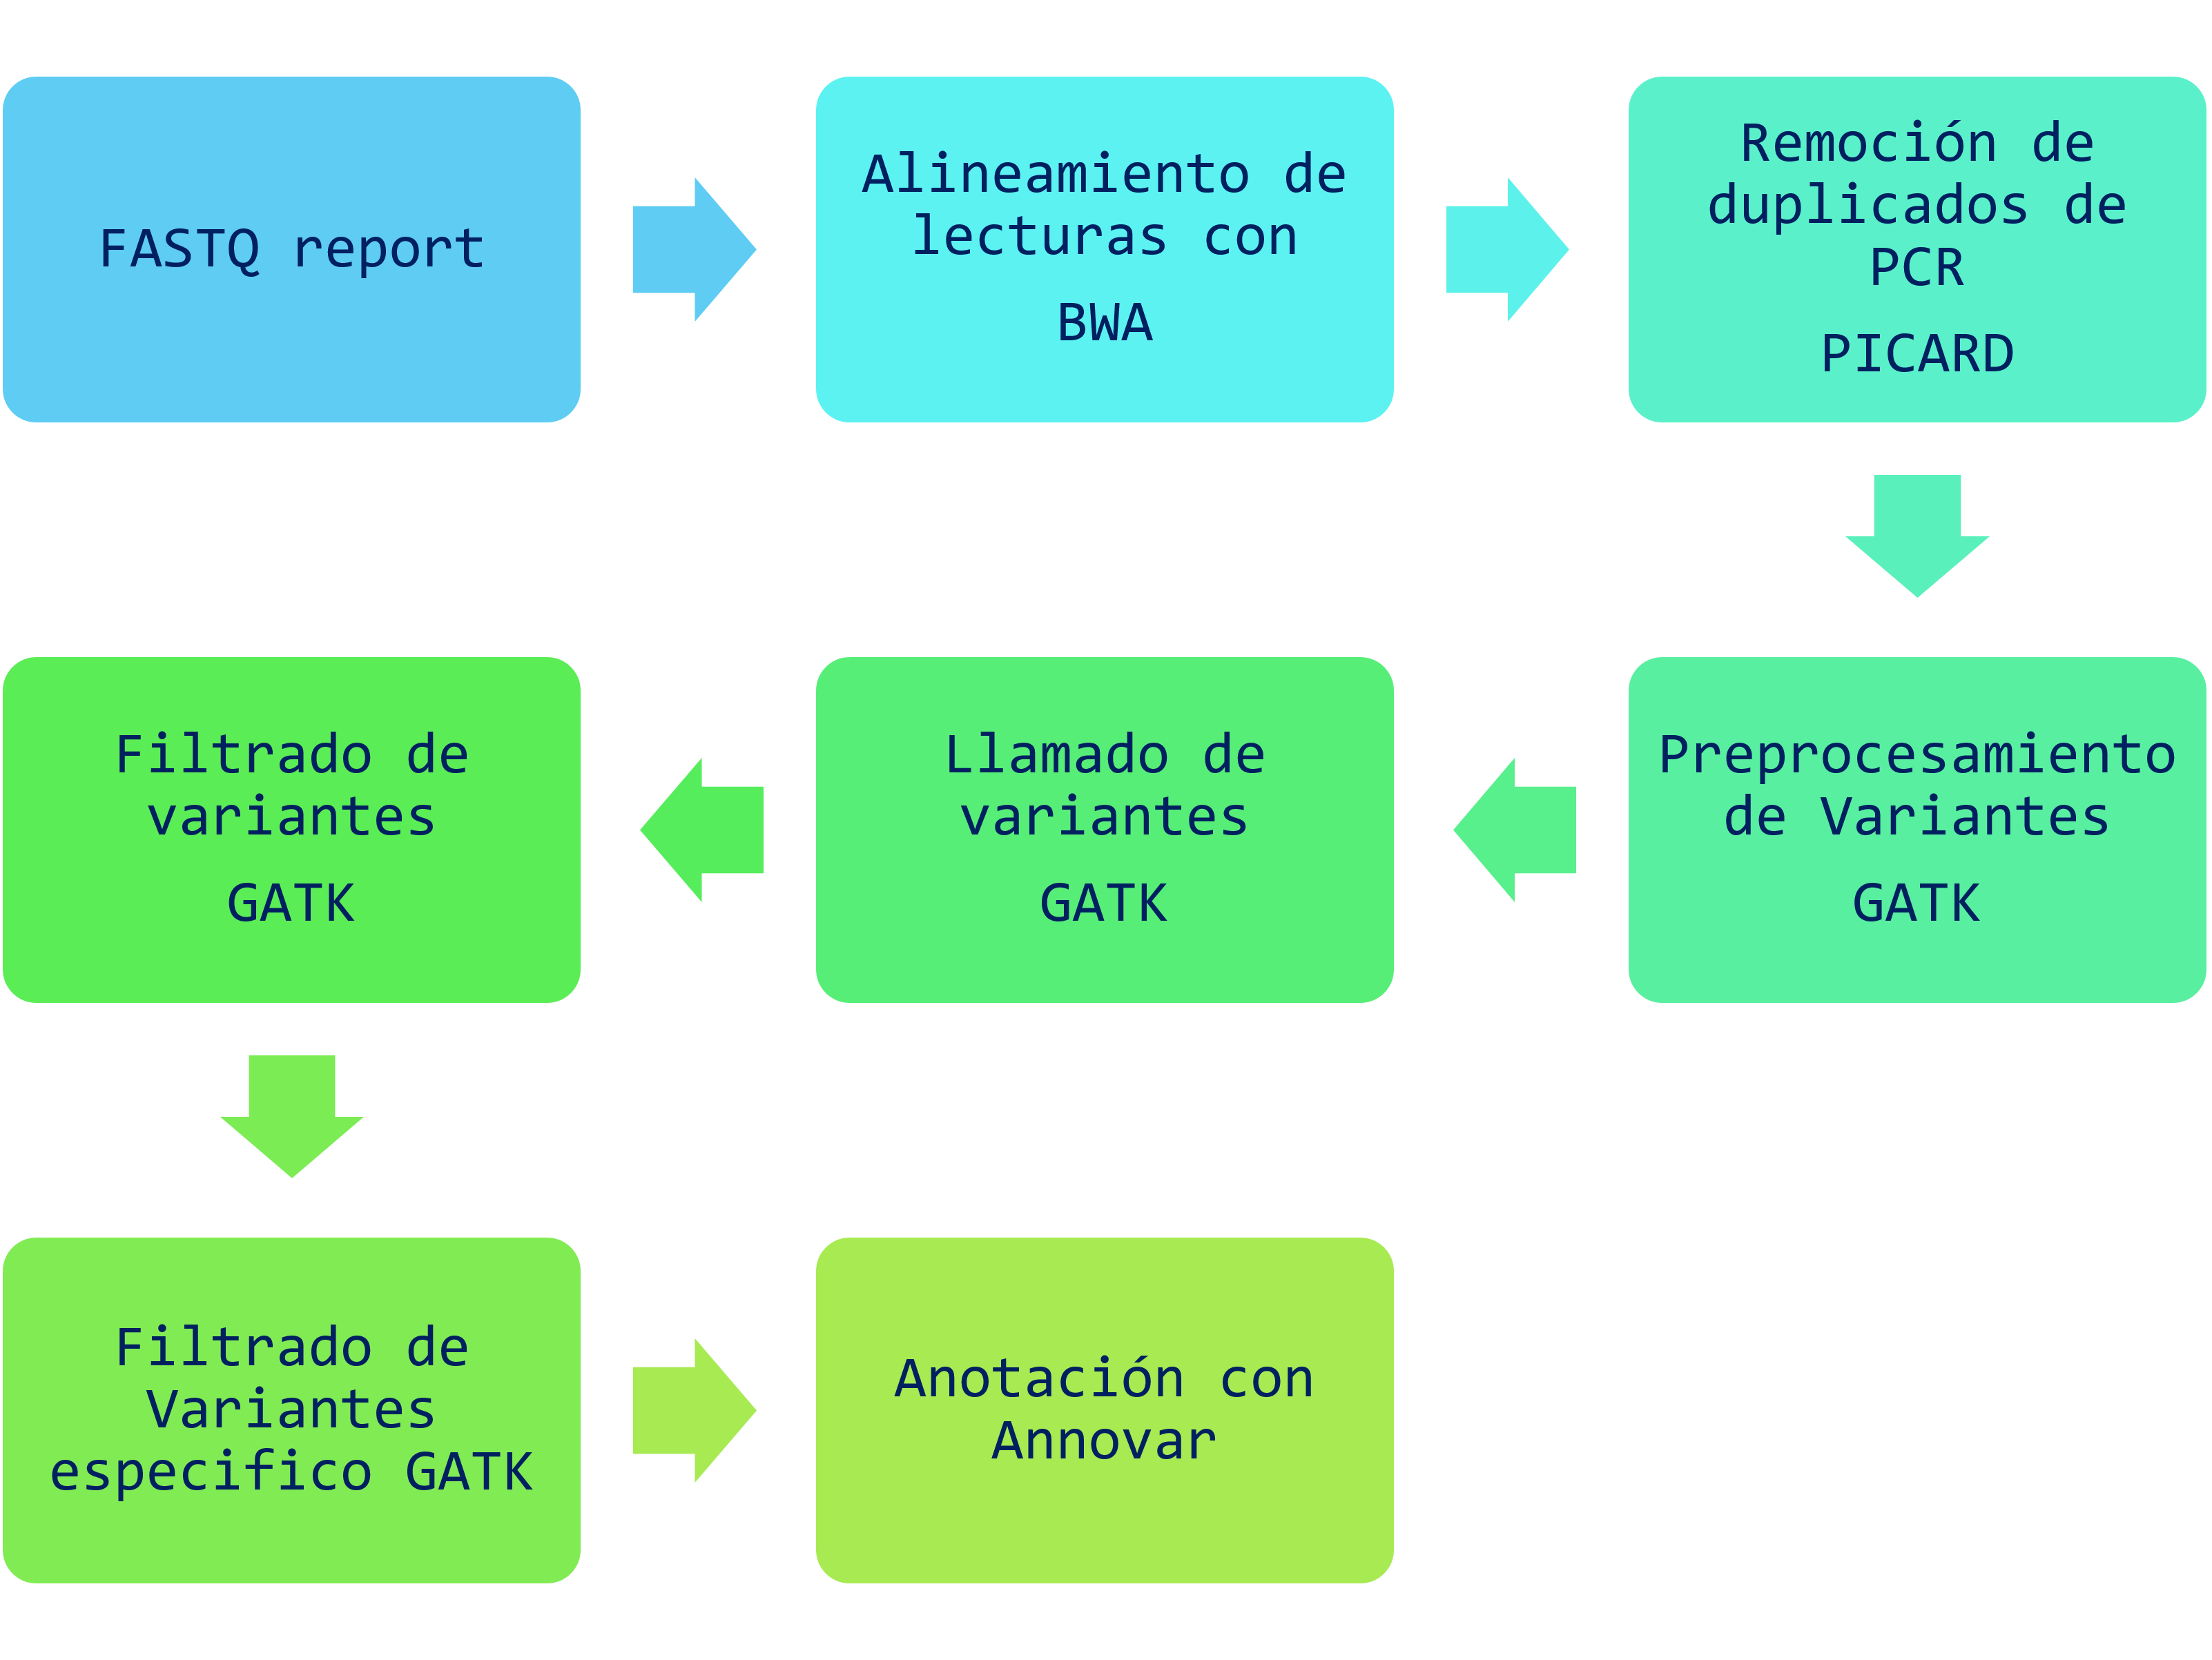
\includegraphics[width=0.6\textwidth]{Kap2/pipeline1}
	\caption{Pipeline base para el llamado de variantes. } \label{fig:pipeline2}
\end{figure}


\subsection*{Herramientas computacionales}
	
	Las herramientas bioinformáticas seleccionadas se implementaron en un clúster \footnote{El clúster utilizado fue prestado por la Universidad de los Andes} que cuenta con las siguientes características:
	
	\begin{itemize}
		\item[$\Rightarrow$] Un nodo master con 2 procesadores Intel Xeon E5-2695 – 24 cores 48 con HT / 192 GB RAM (230Gflops), 300 GB de Disco duro. 
		\item[$\Rightarrow$] Se tienen 19 nodos de trabajo con 2 procecesadores  Intel Xeon E5-2695 – 24 cores 48 con HT / 192 GB RAM (4. 378Tflops), 300 GB de de Disco duro. 
		\item[$\Rightarrow$] Se cuentan con otros 7 nodos de trabajo con 4 procesadores AMD Opteron 6282 SE – 64 cores / 128 GB RAM (3. 659Tflops), 200 GB de Disco duro. 
		
		\item[$\Rightarrow$] 1 GPU tesla K20 como nodo de trabajo con 2 Procesores  Intel Xeon X5690 - 12 cores / 192 GB RAM (3. 659Tflops), 1. 6 TB de Disco duro. 
		
	\end{itemize}
	
Se instaló el módulo para python de omics-pipe, para python 2 con la herramienta de R y las librerías que solicita omics-pipe\cite{Fisch2015}. El algoritmo BWA-MEN samtools, vcftools, GATK 3. 5, picard, FASTQC y pbs-drmma. Una vez instalados los programas se procesaron las muestras dentro del clúster.  


\section{Resultados y validación}
	\subsection*{Reporte FASTQC}}

Este reporte utilizando la herramienta FASTQC presenta inicialmente un resumen del estado de las secuencias obtenidas, ya que toma el archivo fastq y lee las métricas de calidad de cada una de las bases y genera un reporte general en formato HTML. Ya que es interactivo y genera varios módulos \cite{Babraham2016}. \\

Este reporte no presenta fallas dentro del análisis. A continuación se muestra un el primer módulo del reporte FASTQ obtenido de un dato experimental de una secuenciación de 4813 genes que resume el estado general de las lecturas obtenidas para este caso, la figura \ref{fig:fastq2} muestra que la calidad de las secuencias es mayor a 30, el reporte general también muestra que no hay secuencias adaptadoras, que presenta una distribución media del largo de las secuencias aceptable y que no hay secuencias sobre representadas.  \\

\begin{figure}[H]
	\centering
	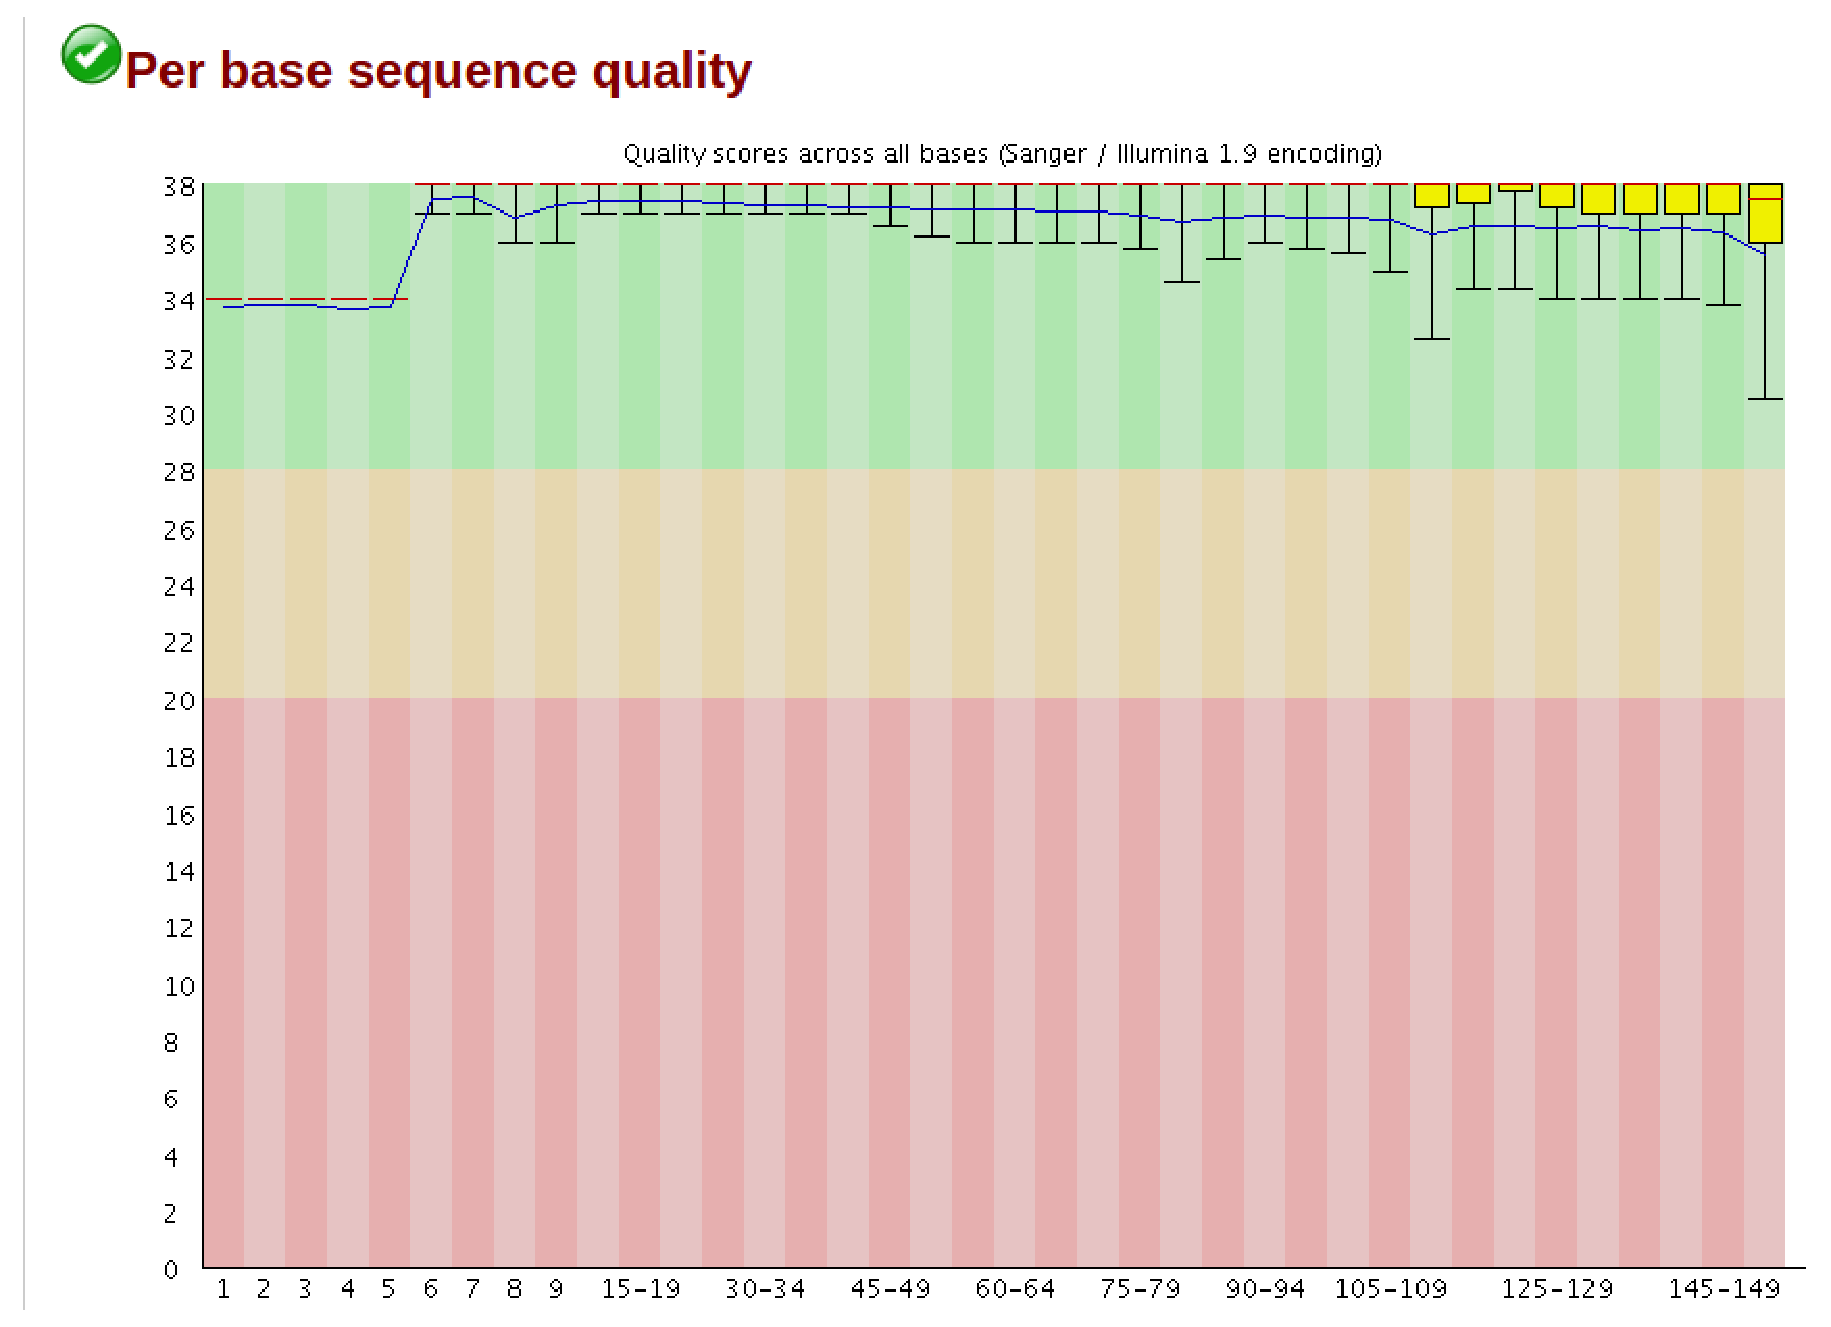
\includegraphics[width=0.4\textwidth]{Kap2/fastq2}
	\caption{Calidad del llamado de bases en una secuencia Estadísticas básicas del reporte FASTQ} \label{fig:fastq2}
\end{figure}

Para el caso de esta muestra la calidad es óptima en todos los datos obtenidos y no requieren de ningún tipo de ``trimming" ya que la mayoría de las posiciones dentro de la secuencia se encuentran por encima del un valor por encima de 34 y el cual el valor mínimo es 20 (este valor representa el ($Q_{PHARED}$) que implementa el secuenciador \cite{Babraham2016}. \\ 

\subsection*{Variantes de illumina vs variantes de Omics}

Inicialmente se obtuvieron 63515 variantes una vez que se ejecuto el pipeline de omics para la obtención de variantes, siguiendo los protocolos de buenas prácticas y los protocolos de GATK quienes recomiendan generar variantes altamente sensibles y poco precisas, esto con el fin de no perder variantes que se encuentren dentro de las secuencias obtenidas, por ello se muestra una gran cantidad de variantes que no corresponden con las variantes verdaderas \cite{Auwera2014}. Dentro del pipeline solo se encuentra el proceso de llamado de variantes y no el proceso de filtrado de las mismas y que debió ser implementado de manera manual. A partir de la aplicación del pipeline se obtuvieron resultados representado en el cuadro \ref{tabla:final}. 

\begin{table}[htb]
	\centering
	\begin{tabular}{|l|l|l|l|l|}
		\hline
		& \multicolumn{4}{c|}{\textbf{Variantes}} \\
		\cline{2-5} 
		& SNP  & Indels & Desconocida & Total \\ \cline{2-5}
		\hline 
		\multirow{1}{4cm}{Variantes Omics} & 54538 & 8855 & 122 & 63515 \\ \cline{2-5}
		\hline 
		\multirow{1}{4cm}{Variantes Calibradas} & 10425 & 828 & 44 & 11297 \\ \cline{2-5}
		\hline
		\multirow{1}{4cm}{Variantes Illumina} & 9601 & 436 & 28 & 10065 \\ \cline{2-5}
		\hline
	\end{tabular}
	\caption{Variantes obtenidas al aplicar pipeline.}
	\label{tabla:final}
\end{table}

De las variantes sin ``hard filtering" se obtuvieron 54538 SNP, Indels 8855 y 122 variantes desconocidas, que se presentan en la figura \ref{fig:omics}: 

\begin{figure}[H]
	\centering
	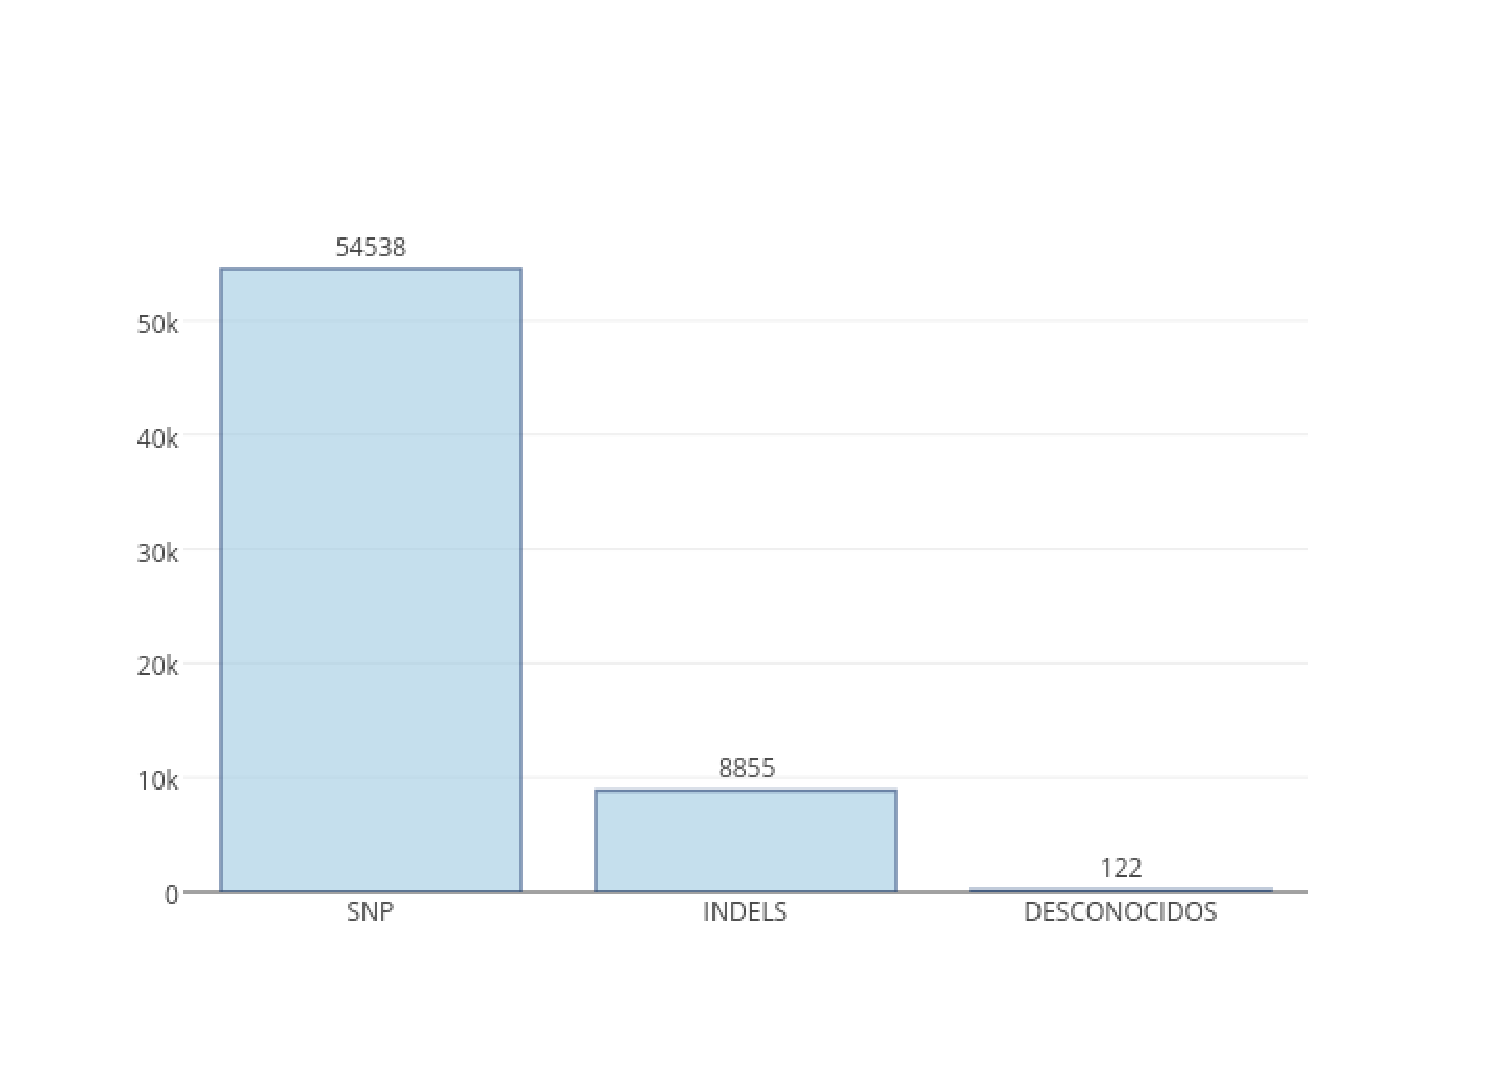
\includegraphics[width=0.5\textwidth]{Kap2/variantesomics}
	\caption{Variantes obtenidas por pipeline} \label{fig:omics}
\end{figure}

Una vez realizado el ``hard filtering" se obtuvo los siguientes resultados: 10425 SNP, 828 Indels y 44 desconocidos, también se tiene las variantes reportadas para el mismo individuo desde la plataforma de illumina con los siguientes resultados: 9601 variantes, 436 indels y 28 desconocidas y representadas en la figura \ref{f:histogramas}.

\begin{figure}[H]
	\subfigure[Variantes obtenidas mediante calibración]{
		\label{f:omics}
		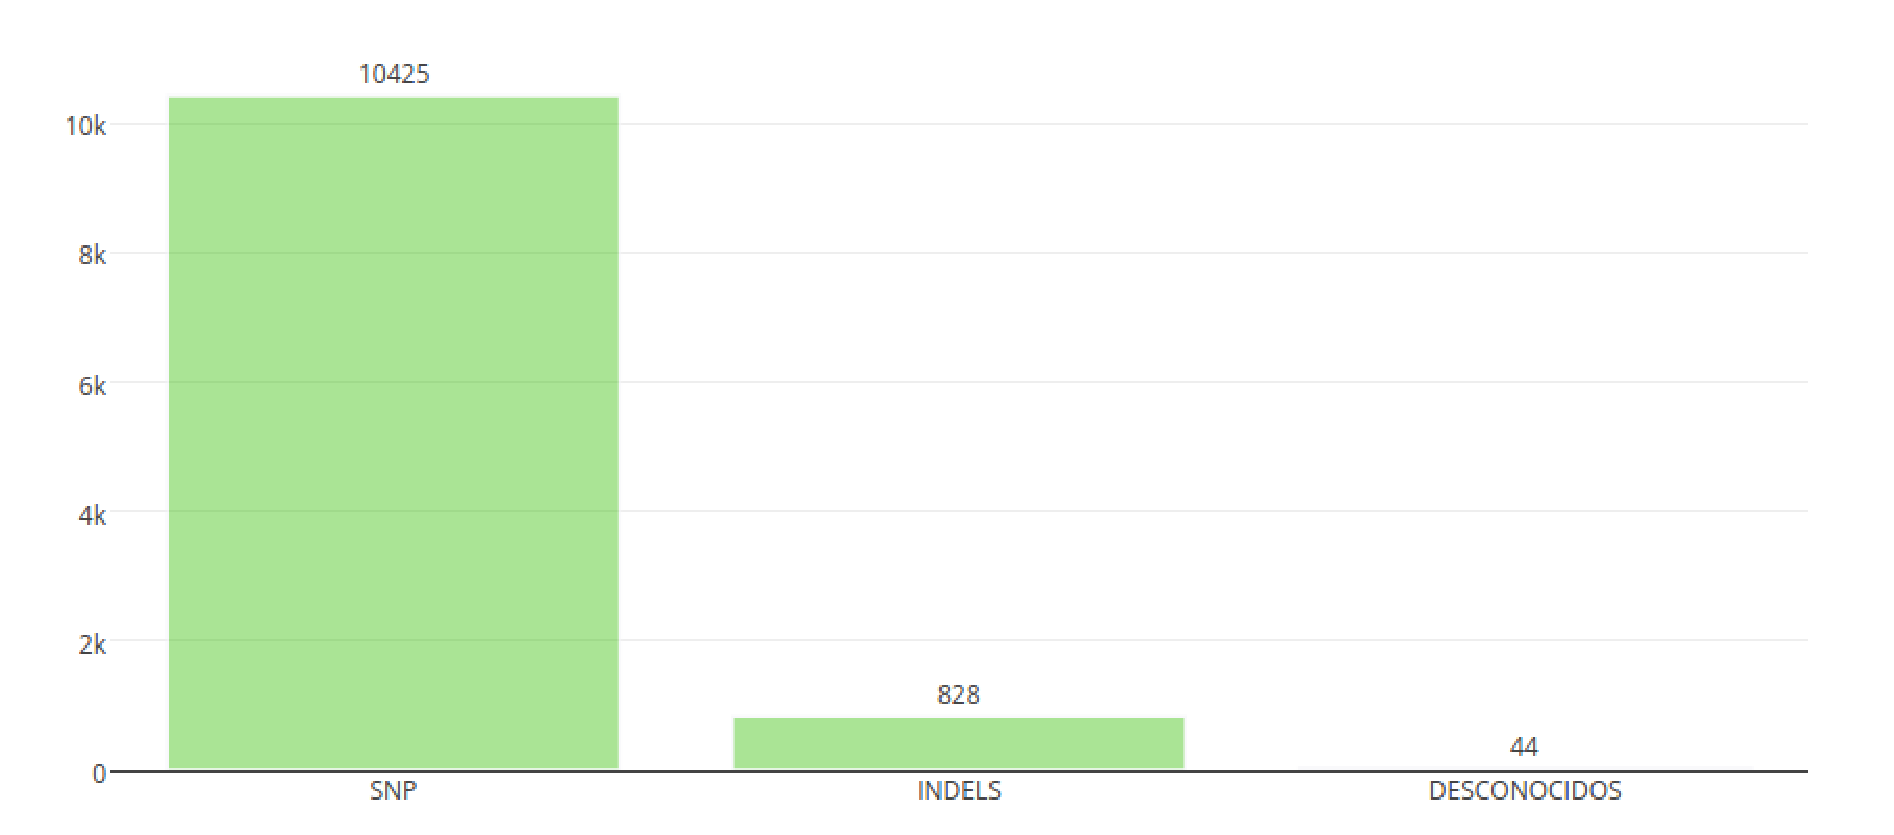
\includegraphics[width=0.5\textwidth]{Kap2/variantescalibradas}}
	\subfigure[Variantes illumina]{
		\label{f:calibradas}
		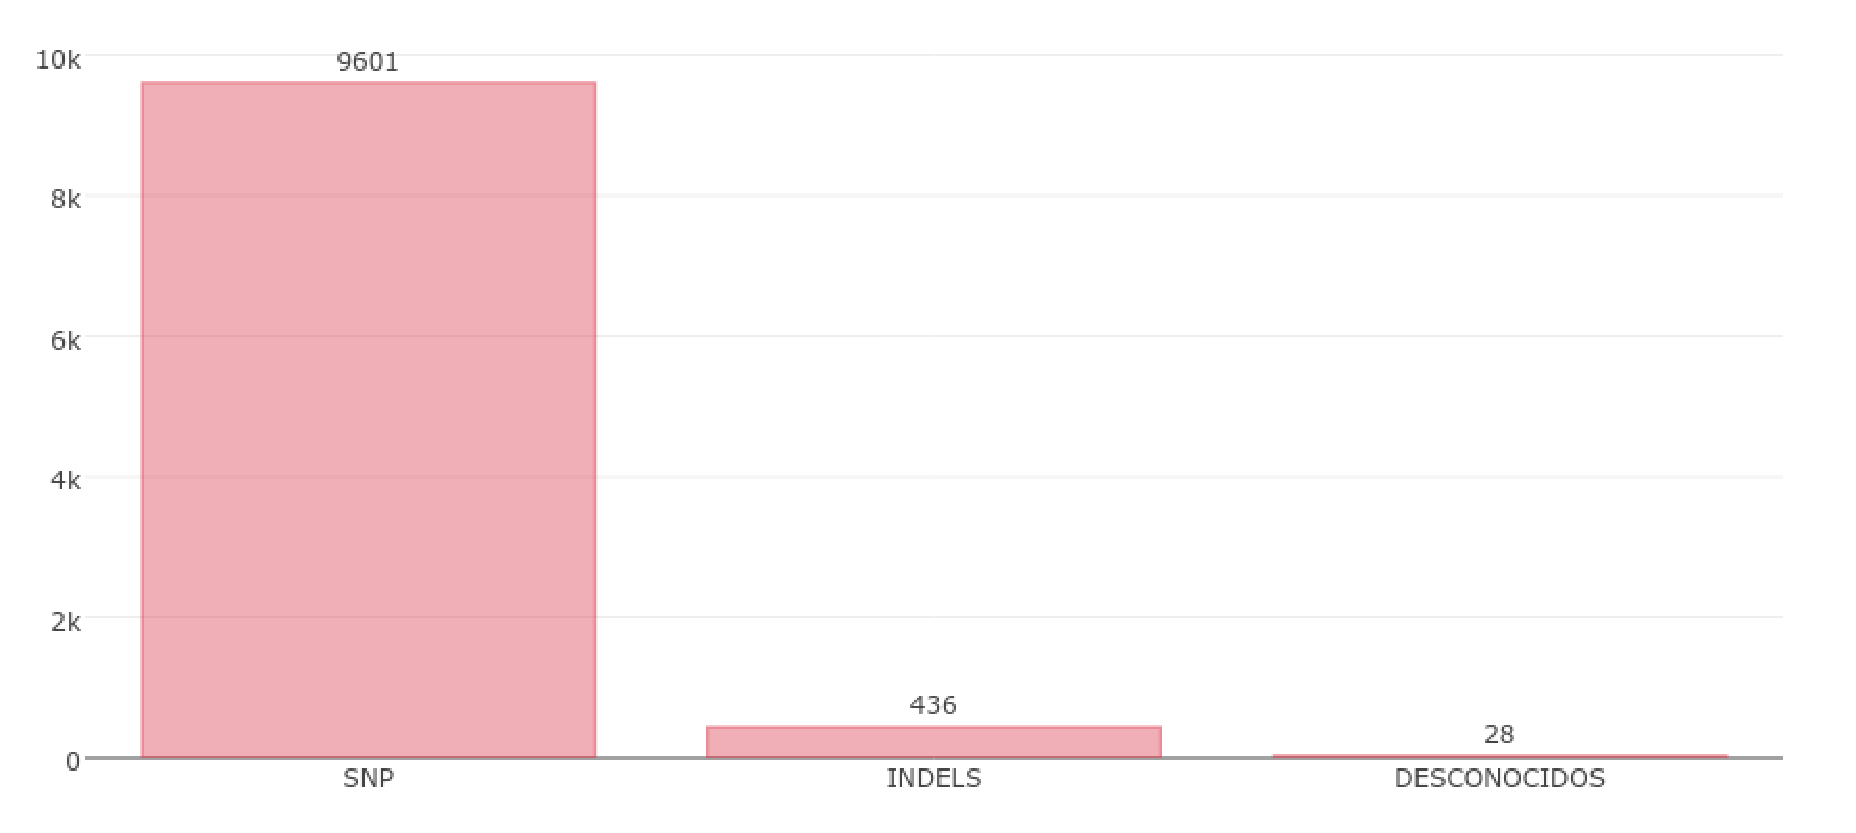
\includegraphics[width=0.5\textwidth]{Kap2/variantesillumina}}
	\caption{Variaciones de la muestra}
	\label{f:histogramas}
\end{figure}

Se realizó una distribución de las variantes según cada técnica sin filtrado (para el caso de omics) para mostrados en las  figuras  \ref{fig:tabla1} y \ref{fig:distribucion}. \\

\begin{figure}[]
	\centering
	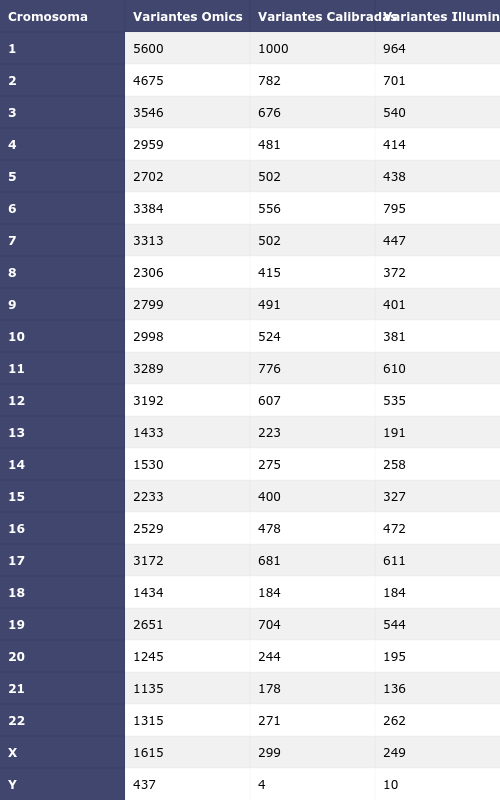
\includegraphics[width=0.4\textwidth]{Kap2/latex_table}
	\caption{Distribución de variantes a lo largo de los cromosomas} \label{fig:tabla1}
\end{figure}

\begin{figure}[]
	\centering
	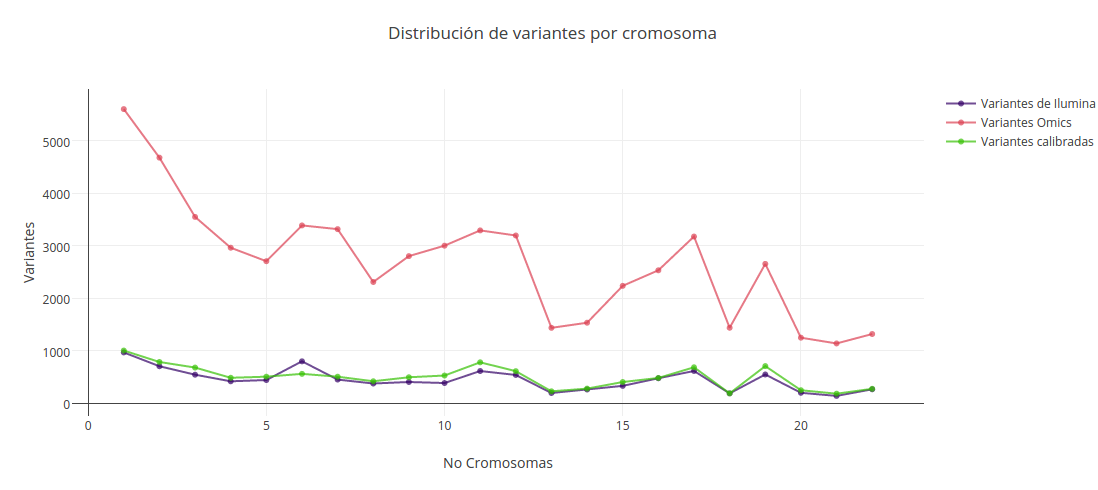
\includegraphics[width=1\textwidth]{Kap2/variaciones}
	\caption{Distribución de variantes a lo largo de los cromosomas.} \label{fig:distribucion}
\end{figure}

Se observa la distribución de las variantes a lo largo del genoma, inicialmente las variantes obtenidas son en grandes cantidades para el modulo de omics, pero conservan el patrón de distribución es similar para los tres casos, incluso cundo se realiza el hard filterin las diferencias en cuanto a la distribución de las variaciones es similar, siendo la mayor para el cromosoma 1 y la menor para el cromosoma Y. \\

Al realizar la comparación entre los dos archivos vcf se obtuvieron los siguientes resultados los archivos vcf de Illumina y los de Omics comparten 49.4 \% d y 44.0 \% de las variantes, y difieren entre un 50.6\% para Illumina y 56-0\% para los datos de omics pipe. Como se refleja la figura \ref{fig:diagrama}. \\

\begin{figure}[]
	\centering
	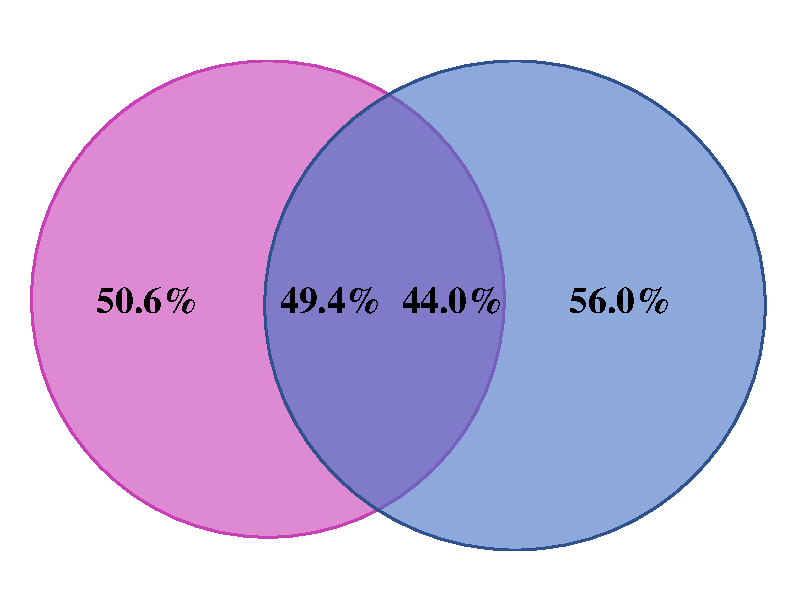
\includegraphics[width=0.3\textwidth]{Kap2/validacion2}
	\caption{Diagrama de relación entre variantes comunes de pipeline y de Illumina} \label{fig:diagrama}
\end{figure}

\subsection*{Variantes de exoma vs variantes de omics}

Una vez obtenidas las regiones se realizó el proceso de ``hard filtering" para el vcf obtenido por el pipe de omics y por el generado por vcftools teniendo los siguientes resultados mostrados por el cuadro \ref{tabla:tabla2}. \\

\begin{table}[H]
	\centering  
	\begin{tabular}{|l|l|l|l|l|}
		\hline
		& \multicolumn{4}{c|}{\textbf{Variantes Exoma}} \\
		\cline{2-5} 
		& SNP  & Indels & Desconocida & Total \\ \cline{2-5}
		\hline 
		\multirow{1}{4cm}{Variantes Omics} & 30893 & 3324 & 0 & 34217 \\ \cline{2-5}
		\hline 
		\multirow{1}{4cm}{Variantes Públicas} & 29749 & 3101 & 0 & 32850 \\ \cline{2-5}
		\hline
	\end{tabular}
	\caption{Variantes obtenidas a partir de un exoma.}
	\label{tabla:tabla2}
\end{table} 

Donde se observa una diferencia de 1367 en el total de las variantes encontradas, para los SNPs se encuentra una diferencia de 1144 y 223 para los indels, no se encuentran variantes que no hayan sido correctamente identificadas. Presentado en los siguientes gráficos \ref{f:histogramas2}. La distribución de las variantes a lo largo de los cromosomas se presenta en la  figura \ref{fig:tabla2}.\\

\begin{figure}[]
	\centering
	\includegraphics[width=0.4\textwidth]{Kap2/latex_table2}
	\caption{Distribución de variantes a lo largo de los cromosomas para los exomas.} \label{fig:tabla2}
\end{figure}

\begin{figure}[H]
	\centering
	\subfigure[Variantes obtenidas por pipeline]{
		\label{f:variantesexo1}
		\includegraphics[width=0.5\textwidth]{Kap2/variantesexo1}}
	\subfigure[Variantes públicas]{
		\label{f:variantesexo2}
		\includegraphics[width=0.35\textwidth]{Kap2/variantesexo2}}
	\caption{Variaciones de la muestras dentro del exoma}
	\label{f:histogramas2}
\end{figure}

La representación gráfica de las variantes sobre la distribución a lo largo de los cromosomas se presenta en la figura \ref{fig:variaciones2}. \\

\begin{figure}[H]
	\centering
	\includegraphics[width=1\textwidth]{Kap2/variaciones2}
	\caption{Distribución de variantes a lo largo de los cromosomas para los exomas} \label{fig:variaciones2}
\end{figure}

En la figura \ref{fig:variaciones2} se observa el comportamiento de la distribución de las variantes para los datos públicos y los datos obtenidos para el pipeline donde se encuentran un comportamiento similar de la distribución, pero se observa que aún hay una mayor cantidad de variantes obtenidas por el pipeline. En la siguiente figura se observa el comportamiento de las variantes públicas con respecto a las variantes del pipeline. \\

\begin{figure}[H]
	\centering
	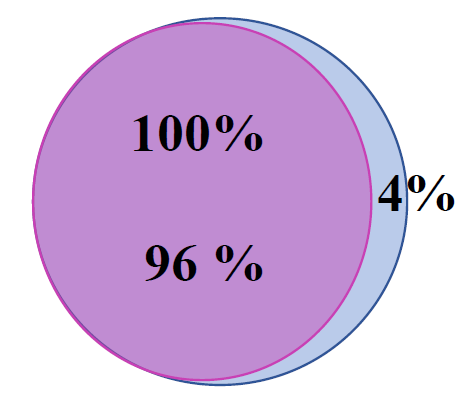
\includegraphics[width=0.2\textwidth]{Kap2/validacion1}
	\caption{Diagrama de relación entre las variantes publicas y las obtenidas por el pipeline.} \label{fig:diagrama2}
\end{figure}

El diagrama de la figura \ref{fig:diagrama2} muestra la comparación entre variantes obtenidas y su respectiva concordancia, donde el 100\% del exoma esta representado en las variaciones encontradas mientras que un 96\% de las variaciones obtenidas por omicspipe corresponden a las variantes del exoma y un 4\% de las variantes no se encontraron dentro del exoma público. \\

GATK realiza un reporte de la evaluación cuando se comparan dos archivos de distintas variaciones, este puede ser abierto como un archivo de texto o cargado directamente en R utilizando la librería \textit{gsalib} que lee el archivo \textit{merged. eval. gatkreport}, esto genera una lista que tiene anidados varios data. frame, dentro de ellos para este caso se tomo el \textit{ValidationReport}. 

El \textit{ValidationReport}  genera una tabla con los verdaderos positivos (\textit{TP}), son las variantes verdaderas definidas como las variantes que previamente han sido identificada en el exoma NA12878, los verdaderos negativos (\textit{TN}), variantes que han sido previamente identificadas pero no son identificadas por el pipeline implementado, los falsos positivos (\textit{FP}) son variantes que no se encuentran en el exoma NA12878, pero que son identificadas por el pipeline y los falsos negativos (\textit{FN}) son las variantes que no están en el exoma NA12878 y que no se identifican, calcula la sensibilidad y la especificidad  y el valor predictivo positivo (PPV). 

\begin{table}[H]
	\begin{center}
		\begin{tabular}{|l|l|}
			\hline 
			\textbf{TP} &  \textbf{FP} \\
			\hline 
			32110 & 1033  \\ \hline
			\textbf{FN} &  \textbf{TN} \\
			\hline
			0 &  0\\ \hline
		\end{tabular}
		\caption{Validación 1. }
		\label{tabla:tabla3}
	\end{center}
\end{table}

El cuadro \ref{tabla:tabla3} refleja que para el conjunto de datos no hay falsos negativos, pero si falsos positivos, es decir  que se obtuvieron 1033 variantes del conjunto de datos que no son reales pero fueron identificadas. (\textit{GATK para calcular estas métricas se compara contra una base de datos que el usuario disponga para determinar variantes existentes}). El cuadro \ref{tabla:tabla4} muestra la sensibilidad, especificidad y el valor predictivo positivo (PPV). 

\begin{table}[h]
	\begin{center}
		\begin{tabular}{|l|l|l|}
			\hline 
			\textbf{Sensibilidad} & \textbf{Especificidad} & \textbf{PPV} \\
			\hline 
			96. 88 & 100 & 100 \\ \hline
		\end{tabular}
		\caption{Validación 2.}
		\label{tabla:tabla4}
	\end{center}
\end{table}

El cuadro \ref{tabla:tabla4} muestra la sensibilidad de 96.88\%, una especificidad del 100\% y un PPV de 100. Además después de realizada la limpieza de los datos se hizo la anotación del archivo vcf obtenido y se filtro para el gen CYP2C19 utilizando la versión gráfica de annovar \cite{Yang2015} y obteniéndose el siguiente resultado: \\

\texttt{chr10, 96541616, 96541616, G, A, exonic, CYP2C19, synonymous SNV, CYP2C19:}

\texttt{NM\_000769:exon5:c. G681A:p. P227P} \\

La representación escrita informa el cromosoma, la posición dentro del genoma y el cambio de posición en el genoma, las siguiente es el cambio Guanina por citocina (representado por sus letras) que es un tipo de variación sinónima, el nombre del gen, su identificador, ubicación exonica y cambio en la posición del exón, finalmente se tiene el cambio en la proteína, la confirmación de que la variante fue encontrada y que es de buena calidad se realizo  con la visualización por medio de la herramienta IGV conectado al clúster como muestra la figura \ref{fig:igv} que muestra el cambio de una G por una A en estado heterocigota. 

\begin{figure}[H]
	\centering
	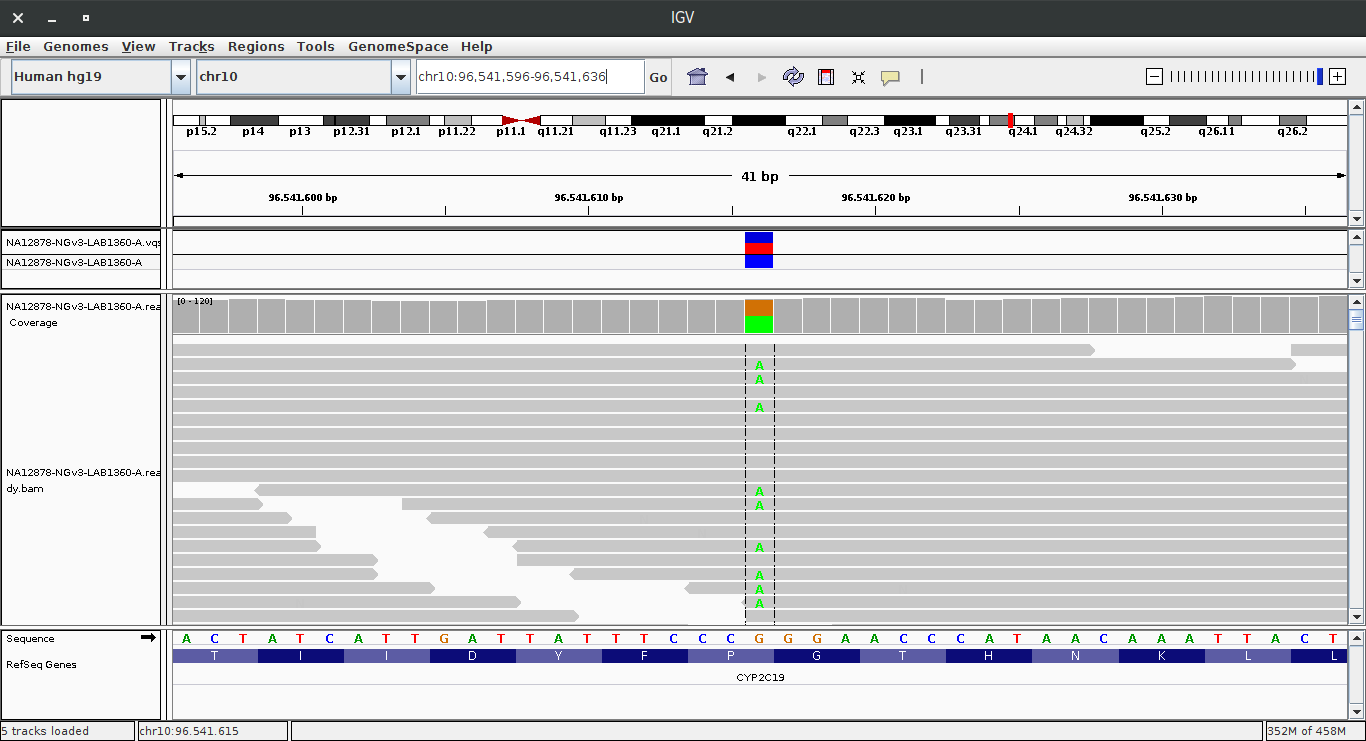
\includegraphics[width=1\textwidth]{Kap2/IGV}
	\caption{Imagen de la variante presente en el exoma público} \label{fig:igv}
\end{figure}

\section{Discusión}

\subsection*{Preprocesamiento}

La revisión de las metricas dadas por el FASTQC report muestran el estado de como están las secuencias antes de ser procesadas, aunque a nivel experimental no dependiendo de las condiciones y el tipo de muestra los niveles de calidad terminan bajando de manera sustancial y depende del analista tomar la decisión de remover secuencias o mantenerlas ya que los diferentes módulos presentan diversas meticas de evaluación de las secuencias \cite{Babraham2016}. \\

El presente conjunto de secuencias FASTQ se encuentra con buenos parámetros de calidad, aunque algunos módulos presentan falla, el percentil, el porcentaje de GC, la distribución del largo de las secuencias, los niveles de duplicación de las secuencias y los valores de K-mer y las secuencias en secuencias cortas de 7 nucleótidos, representan que dentro del conjunto de datos estas secuencias cortas están en la parte inicial de la mayoria de las lecturas obtenidas en la muestra y que posiblemente son secuencias duplicadas que no pertenecen al conjunto de secuencias real, a pesar de que no se encuentran adaptadores, ni representaciones al final de las lecturas. Esto puede llevar a dos caminos, el primero que estas secuencias sean parte de un adaptador (llama la atención que no se encuentren al final de la secuencia)  o que sean errores propios del proceso de secuenciación durante la hibridación de las secuencias y sean representados como duplicaciones de las secuencias originales \cite{Babraham2016}\cite{Pirooznia2014}. \\ 

Además existen otras características que pueden generar impactos negativos dentro del análisis de datos de NGS divididas en dos grupos \cite{Zhou2013}: 

\begin{enumerate}
	\item Lecturas con baja calidad: Las calidades de las lecturas generadas por un secuenciador pueden degradarse durante el proceso de corrido y es común ver fallas al final de la lectura o tener secuencias duplicadas a partir de la amplificación por PCR durante la construcción de las librerías \cite{Zhou2013}. 
	\item Contaminación de las lecturas de especies conocidas o no conocidas en la secuencia objetivo, este error es frecuente y puede se causado por un experimento artificial durante la preparación de la muestra, la construcción de la librería o otro paso experimental, sin embargo las muestras de ADN pueden contener algunos nucleótidos de otras especies, las cuales son difíciles de excluir de manera experimental y por lo tanto si se cree que hay una contaminación, lo ideal es realizar un ``trimming" de las secuencias para remover la contaminación. \textbf{Nota:} Siempre y cuando estén en una baja proporción \cite{Zhou2013}. 
\end{enumerate}

Las secuencias que se  observan pueden ser duplicados de PCR que son un problema crítico cuando los fragmentos están sobre amplificados durante la preparación de las librerías, estos duplicados pueden aumentar a frecuencia alélica e incluir una detección errónea de variantes, esto es muy común los datos de metagenomica, pero en nuestro caso los datos no son datos de metaegenómica si no de un solo individuo llama la atención de que solo estén al inicio de las lecturas y que el final de las lecturas este adecuado esto podría indicar que más que un duplicado de PCR pueda ser un error de secuenciación al inicio de cada nuevo ciclo. \cite{Pandey2016}. \\

Teniendo en cuenta lo anterior se puede inferir que las secuencias duplicadas son bajas y que la calidad de los datos obtenidos son adecuados para continuar con el procesamiento de las secuencias FASTQ, dentro del pipeline se cuenta con una herramienta para remover las secuencias duplicadas (PICARD) y así obtener una calidad optima de los datos. 

\subsection*{Variantes obtenidas}
\subsubsection*{Variantes de illumina y omics pipeline}

En los datos obtenidos para illumina inicialmente reflejados en la tabla \ref{tabla:final}, muestran una alta discordancia ya que inicialmente las variantes no se les aplicó un segundo filtro, siguiendo las recomendaciones de GATK, donde por el pipeline de Omics tiene por defecto el variant quality score racalibration (VQRS) que se basa en machine learning para filtrar las variantes y generar una alta sensibilidad, que es el método más recomendado, pero tiene limitaciones estadísticas y es más robusto que el hard filtering, este es recomendado para datos pequeños \cite{Auwera2014}. \\

Al realizar una calibración de los datos con la calidad y con hard filtering en GATK se obtiene una similitud entre la cantidad de variantes obtenidas por omics pipe con respecto a Illumina, pero aún es posible ver que la distribución de las variantes es similar para ambos conjuntos de datos (véase la figura \ref{fig:distribucion}) y se ve una mayor similitud  después de realizar el filtrado. Esto se presenta debido a que no existe una formula para determinar cuales anotaciones y filtros son adecuados, además el VQSR genera datos de entrenamiento para determinar las variantes. Por esta razón se hacen recomendaciones según lo que se ha observado empíricamente dentro del desarrollo de los algoritmos \cite{Auwera2014}. \\

A pesar de que la distribución de las variante es similar, aun con el filtrado de las variantes existe que la concordancia entre ambas técnicas tiende a ser del 50\% (véase la figura \ref{fig:diagrama}), aunque illumina utiliza GATK la versión implementada es la 1. 6 que en este momento no cuenta con documentación (https://www. broadinstitute. org/gatk/guide/version-history) que illumina utiliza la versión 1. 6 y la función UnifiedGenotyper que presenta algunas inconsistencias para la identificación de indels, mientras que la versión de GATK 3. 5 utiliza la función HaplotyperCaller que mejora el llamado de variantes, y corrige algunas inconsistencias para la identificación de indels \cite{ORawe2013}. Además es la función recomendada para organismos diploides, este se enfoca en dos tipos de identificación inicialmente los SNPs y los indels, y puede identificar cuando hay varios tipos de variantes cercanas a otras \cite{Auwera2014}. \\

Illumina no provee los parámetros utilizados para hacer el llamado de variantes lo que dificulta la comparación entre este pipeline y las variantes reportadas por illumina, además el formato del VCF es el 4. 1 y en la mayoria de las variantes no reporta el valor de la Qual (calidad) para hacer un filtro con el archivo aunque para GATK los valores para el llamado de variantes no son modificados de manera significativa si se realiza un filtro de este tipo \cite{Hwang2015}. Además de que la combinación de BWA con HaplotypeCaller, presentan una mejora con respeto a la identificación de SNPs (BWA-men) y HaplotypeCaller para la identificación de indels \cite{Cornish2015}. 

\subsubsection*{Variantes con un exoma NA12878.}

Para este trabajo se utilizó una muestra del genoma completo de la muestra NA12878 son de 34, 886 variaciones \cite{Cornish2015} en el presente estudio 32850 y el pipeline obtuvo un total de 34217, lo que permite inferir que las variante identificadas son solo de 2036 variaciones (dependiendo de las muestras y los genes que fueron secuenciados) y que se realizó un muestreo partir de un archivo bed. Además si se aplica un filtro para retirar las variaciones con baja calidad, el llamado de variantes de GATK mejora de manera significativa si necesidad de hacer cambios en el preprocesamiento de los datos \cite{Warden2014} \\

Las dos resultados presentan una distribución similar en cuanto a las variantes por cromosoma y no hay variantes desconocidas dentro de la muestra, esto se debe a la alta curación que tiene este exoma, la figura \ref{fig:variaciones2} presenta la distribución a lo largo de los cromosomas donde se presenta leves diferencias entre los datos públicos y los datos generados por el pipeline con una diferencia del 4\% entre las dos resultados, no existen falsos negativos ni verdaderos negativos identificados dentro del conjunto de los datos del pipeline, se presenta una sensibilidad del 96\% que es una buena, dado que las calibraciones y los algoritmos presentan falencias reales para la identificación de variantes \cite{Auwera2014}. Esto se puede corregir por dos vias, aplicando un filtro de Quality by Depth (QD) >= 4 and Fisher Strand Bias (FS) =< 30 para dar un balance  a la sensibilidad y la especificidad \cite{Tsai2016} o aplicando múltiples pipelines. \\


La sensibilidad de un solo pipeline esta en promedio de 95\% al 99\% , que esta dentro del rango de aceptabilidad para la identificación de las variantes \cite{Liu2013}. Para nuestro pipeline tenemos una precisión de 100\%. Lo que nos indica que hay  una baja probabilidad de error. \\

Al realizar la anotación se logro encontrar una de las variantes reportadas para el exoma, en el gen CYP2C19 en la misma posición reportada, con la misma variación mostrando la concordancia entre los resultados del pipeline y la muestra original. \\

Para ambos estudios se presentan archivos intermedios de gran tamaño como son los bam y bai que permiten la visualización de las variantes que pesan entre 6 y 15 gigas para un exoma completo, los datos iniciales pueden pesar entre 1 y 3 gigas (fastq) dependiendo de la cantidad de genes que se hallan secuenciado, lo que requiere de la disponibilidad de un computo para su almacenamiento y procesamiento. 

\section{Conclusiones}

La validación de un pipeline para la identificación de variantes requiere la utilización de herramientas computacionales de HPC para hacerse de manera eficiente. Es necesario que se tengan conocimientos de programación básica y biología molecular, con el fin de definir los parámetros óptimos para la implementación un pipeline. \\ 

La cantidad de herramientas y parámetros para aplicar son diversos y dependen del investigador decidir cuales son los mejores y que filtros van a ser utilizados, dado que a pesar de la existencia de protocolos no hay un consenso de cual o cuales son los mejores y estos dependen del conjunto de datos obtenido. \\ 

El llamado de variantes es bueno para el presente estudio, pero hay la posibilidad de mejorar la implementación de los parámetros de filtrado y el proceso de anotación (implicación del cambio de las variantes), además generar un pipeline alternativo para la verificación de las variantes que están siendo identificadas y poder aumentar la sensibilidad. \\

Es necesario crear o generar la manera de optimizar los tiempos de ejecución de las tareas de una manera más eficiente a la dada por el omics-pipe. 

\section*{Resumen}

Se realizó la implementación y validación de un pipeline para la identificación variantes a partir de secuencias de exomicas a partir de muestras de pacientes colombianos y del genoma público de la muestra NA12878 donde se identificaron las variantes que están presentes en el mismo, teniendo en cuenta las buenas practicas para el llamado de variantes lo que permitió desarrollar un mecanismo para obtener variantes de buena calidad. 
\chapter{Modelo de Integración de la Información}
\section{Introducción}

Las nuevas tecnologías de análisis genético son fáciles y económicas de hacer lo que genera una gran cantidad de datos biológicos y lo que hace que los biólogos trabajen cada vez más con las nuevas tecnologías de análisis genético, haciendo que los biólogos trabajen más y más computacionalmente.Especialmente mediante el uso de  tecnologías de secuenciación (NGS) y presentar un reto para integrar y almacenar la información, pasos que son necesarios para su posterior análisis \cite{Li2014,Cook2016}.\\

La gran cantidad de datos presentan un reto para organizar y manejar datos que crecen de manera exponencial y que son de diversos tipos, dado que los datos son generados a diferentes niveles y con diferentes métodos (ejemplo: Variantes de exones o imágenes de patología), datos que a su vez deben ser almacenados en distintas formas, esta situación muestra una seria dificultad para realizar un análisis integral de los datos \cite{Cook2016,Li2014}.\\

El mayor de los retos es crear herramientas que permitan al investigador acceder a la información fácilmente y que pueda tener una base de datos intercalable,donde pueda consultar, analizar y actualizar la información de sus experimentos \cite{Li2014}.En el campo clínico esto representa un reto aun mayor dado que se hace necesario recolectar los datos genéticos junto con los datos clínicos para poder hacer análisis más acertados y a gran escala \cite{Paila2013}.\\

El problema de la heterogeneidad  de los datos  se aplica igualmente a los datos clínicos que describen pacientes individuales y además a los datos biológicos que caracterizan nuestro genoma. Específicamente la información genómica y clínica son datos altamente heterogéneos con respecto a los modelos de datos que emplean normalmente, los esquemas de datos que especifican, los lenguajes de consulta que soportan y las terminologías que reconocen \cite{Sujansky2001}.\\

Para el caso de las variantes se tiene que para cada individuo hay 3.5 millones de variantes por individuo, estas variantes son almacenadas normalmente en el formato VCF (Formato de llamado de variantes), a su vez estos archivos pueden contener varias gigas de información,especialmente las muestras de genomas completos, que representan un problema para el almacenamiento dentro de las bases de datos, bases de datos que han sido desarrolladas para dar soluciones dependientes de las diferentes características y necesidades de los laboratorios\cite{Kutzera2017}.\\

Por ello se hace necesario que se utilicen herramientas para la gestión de la información, por ejemplo django que es un web framework de alto nivel desarrollado en python  fomenta el desarrollo rápido y limpio, para la creación de aplicaciones web, es de código abierto y gratuito.Se basa en los principios de desarrollo rápido, manejo de la seguridad y es altamente escalable . Dentro de las muchas aplicaciones que tiene django una es el manejo y gestión de bases de datos a través de los módulos de python. Ver documentación https://www.djangoproject.com/. 

\section{Metodología}

A continuación proponemos la utilización de una base de datos con la información clínica disponible y las anotaciones de variantes obtenidas por medio de un pipeline que fue validado previamente (la validación se encuentra descrita en el siguiente capitulo) para la anotación de variantes, basado en la propuesta de Fish y colaboradores en 2015 \cite{Fisch2015} y anotados con annovar web service \cite{Yang2015}. Las historias clínicas fueron transcritas manualmente y cargadas desde un archivo de texto plano con un formato especifico.\\

Se genero una base de datos utilizando Django 1.10 en python 3 y la librería grapelli, que se conectan  a  MySQL  5.7.17 desde un PC portatil HP-pavilion 360 con ubuntu 16.04 LTS. Django genera los modelos de EER pero permite su modificación para optimizar la velocidad de las consultas. \\

La figura \ref{fig:flujo2} representa el flujo de trabajo que fue utilizado para realizar la integración de la información dentro de la base de datos.

\begin{figure}[H] 
	\centering
	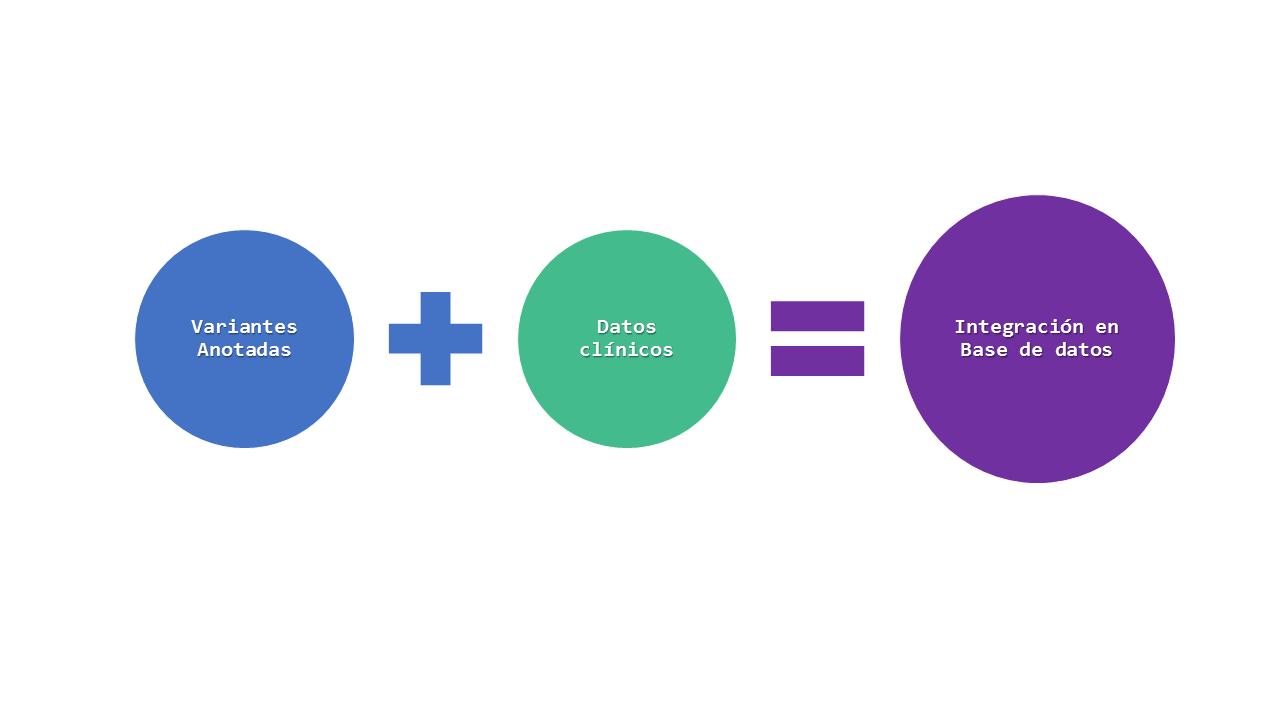
\includegraphics[width=0.6\textwidth]{Kap3/flujo2}
	\caption{Flujo de integración de la información.} 
	\label{fig:flujo2}
\end{figure}

Las variantes con su historia clínica fueron cargadas mediante un script en bash disponible en https://github.com/jevelezse/variantesBD/blob/master/carga.bash, donde se toman los archivos .csv de annovar junto con los archivos de texto que tienen la información clínica del paciente distribuida de la siguiente forma:

\begin{itemize}
	\item Edad: 0-99. Los recién nacidos  o menores de un año tienen una edad de 0.
	\item Sexo: F o M según corresponda.
	\item Descripción: Que corresponde a la información clínica disponible.
\end{itemize} 

\section{Resultados} 

Los resultados obtenidos fueron una aplicación con una interfaz que permite a los usuarios con poco conocimiento de  programación  analizar los datos de variantes y su resumen de la historia clínica. \\

\begin{figure}[h] 
	\centering
	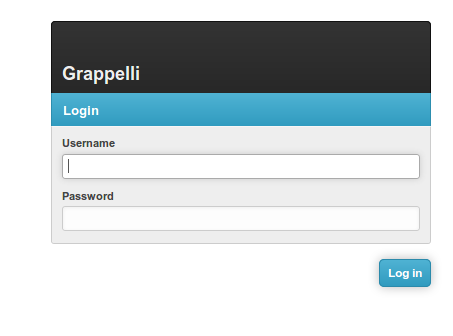
\includegraphics[width=0.4\textwidth]{Kap3/admin_django}
	\caption{Interfaz de ingreso para  administrar la base de datos.} \label{fig:admin}
\end{figure}

Inicialmente la figura\ref{fig:admin}, muestra la solicitud de usuario y contraseña para acceder a la aplicación, es diferente a la base de MySQL, pero  puede tener  una contraseña igual o diferente a la de la base de datos.

\begin{figure}[h] 
	\centering
	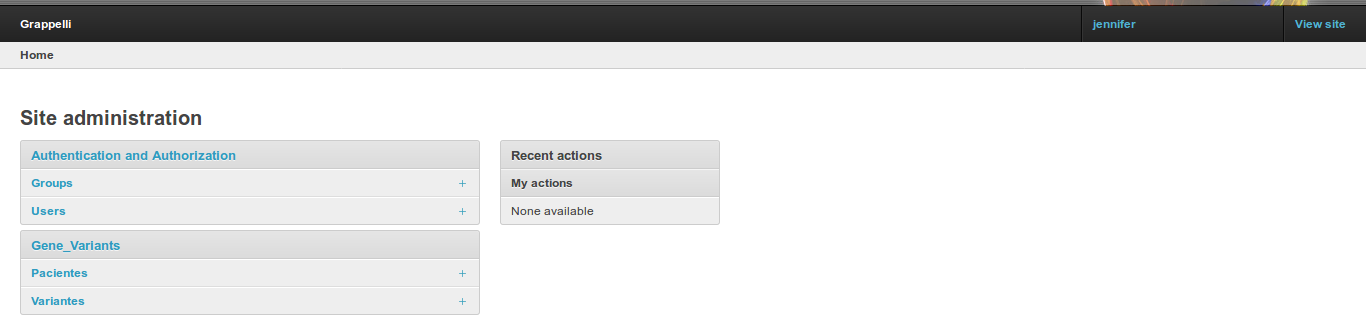
\includegraphics[width=0.5\textwidth]{Kap3/django_admin}
	\caption{Interfaz de administración.} \label{fig:admin2}
\end{figure}

La figura \ref{fig:admin2}, muestra el sitio de administración donde se encuentran los usuarios permitidos, las bases de datos a consultar y muestra un histórico de las actividades recientes. \\

Desde esta interfaz se puede agregar un grupo, más usuarios, pacientes y/o variantes dando click en el signo más sin necesidad de hacer la carga directa a MySQL ya que Django se encarga de hacer la carga, lo que permite actualizar los cambios que se reporten para la variante, por ejemplo variantes que por su alta frecuencia poblacional dejan de ser variantes y se convierten en referencias. \\

\begin{figure}[h] 
	\centering
	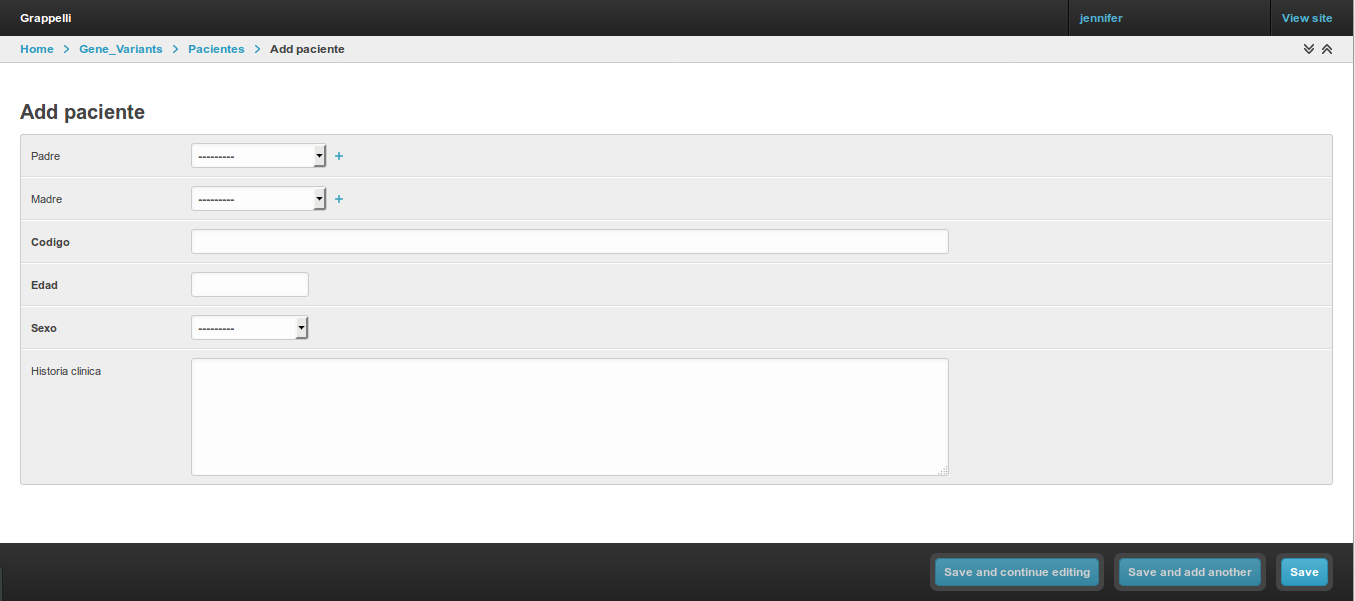
\includegraphics[width=0.5\textwidth]{Kap3/ingresar_paciente}
	\caption{Ingreso de pacientes.} \label{fig:pacientes}
\end{figure}

En la figura \ref{fig:pacientes} se muestra el formulario para ingresar una nueva historia o de modificar una historia clínica de un paciente de manera manual.

\begin{figure}[h] 
	\centering
	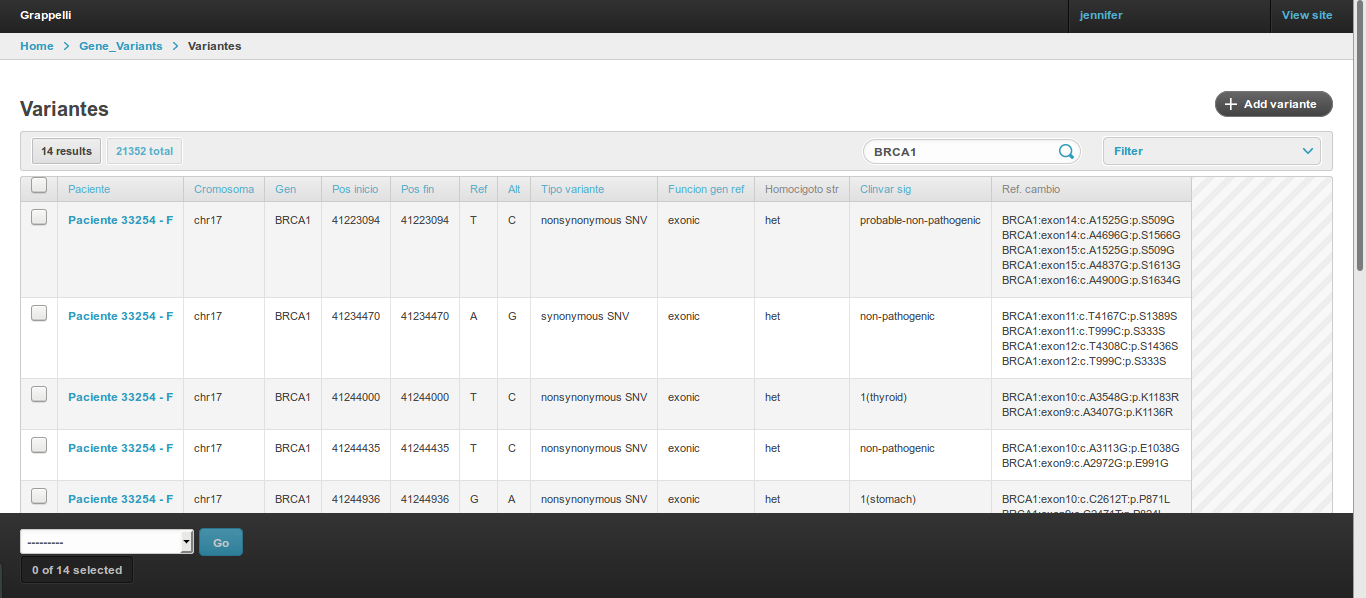
\includegraphics[width=0.5\textwidth]{Kap3/consulta}
	\caption{Consulta a variantes} \label{fig:consulta}
\end{figure}


La figura \ref{fig:consulta} muestra una consulta de las variantes que se tienen cargadas en la base de datos para el gen BRCA1, donde nos muestra una consulta de las variantes con su anotación  filtrada mediante un script de python antes de cargar las anotaciones de la tabla obtenida por annovar para cada paciente. Desde esta misma interfaz se puede hacer consultas de pacientes que se deben eliminar, en la parte inferior se encuentra la opción.\\

Si se desea hacer modificaciones a los datos del paciente también es posible hacerlo desde esta misma interfaz seleccionando el código del paciente, que lleva a la tabla de genes\_varante\_paciente que contiene el formulario de la historia clínica con los datos cargados para ser modificados. 

\begin{figure}[H]
	\centering
	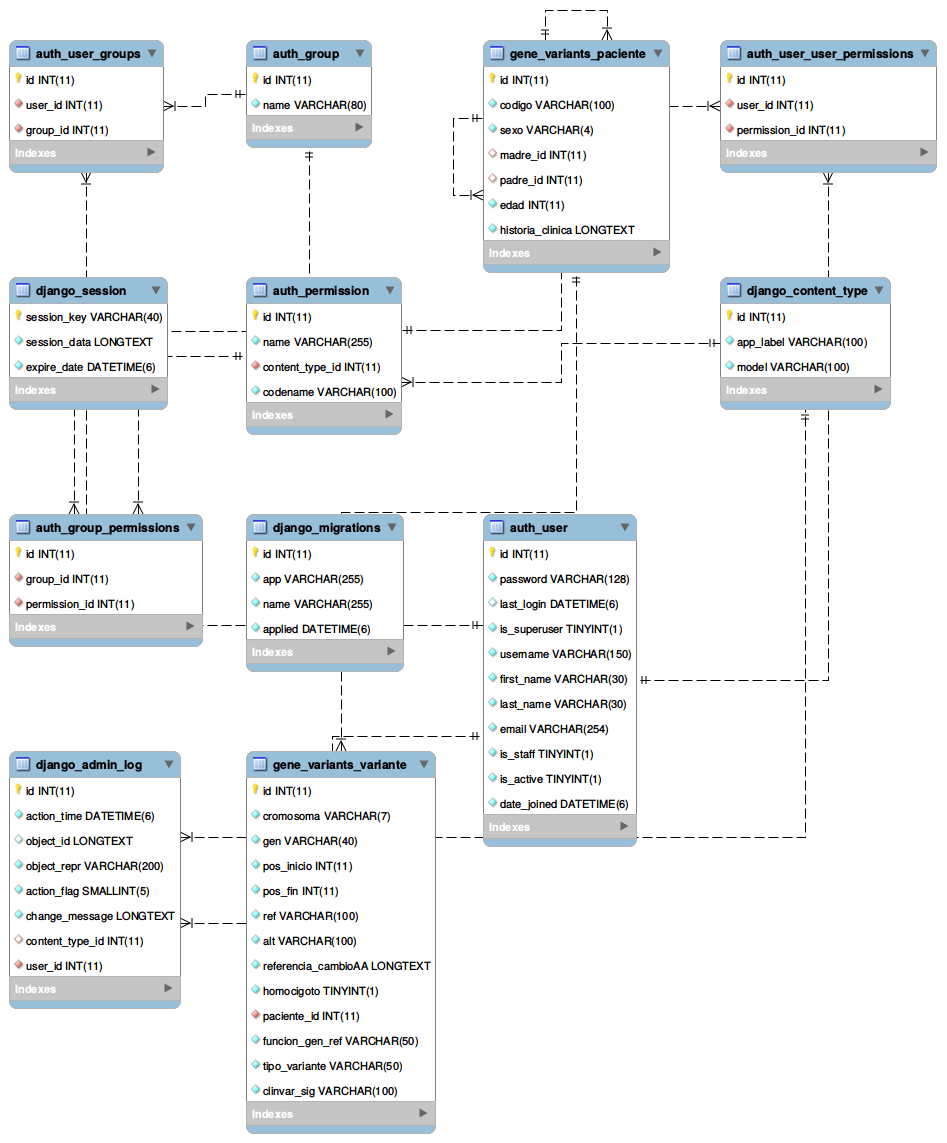
\includegraphics[width=0.9\textwidth]{Kap3/modeloEER}
	\caption{Modelo entidad relación} \label{fig:t}
\end{figure}

La figura \ref{fig:t} muestra el modelo EER que se genero en la base de datos MySQL, donde se muestra el modelo  EER que muestra las tablas generadas por la aplicación para crear la base de datos donde se incluyen las tablas de para la gestión del las variantes junto con la historia clínica y se tiene encuentra la posible relación parental, padre, madre e hijo, el control de las consultas de la variantes indexadas y dentro de la misma base la gestión de accesos a otros usuarios con sus permisos.

\section{Discusión}

\subsection*{Gestión de datos genómicos y clínicos}

La importancia de gestión aplicada al manejo de datos clínicos y de información genética es de vital importancia dado que existen miles de anotaciones que requieren de scripts para cargarlos las anotaciones y como es este caso el historial clínico del paciente \cite{Paila2013}. \\

La aplicación desarrollada para crear y gestionar una base de datos aplicada una bioinformática con aplicaciones a la medicina, es necesario que la base de datos provea las consultas para soportar las decisiones sobre un paciente en especifico teniendo en cuenta sus datos,la relación con datos de otros pacientes y los datos de exomas, además de los datos relacionados con los familiares en caso de que se encuentren estos datos. Mostrando que es posible realizar una integración adecuada de los datos bioinformáticos y clínicos utilizando bases de datos relacionales, con una buena respuesta en las consultas. \cite{Sujansky2001}.

\section{Conclusión}

La utilización de aplicaciones en Django permite que un bioinformático diseñe e implementar bases de datos aplicadas al diagnostico clínico, donde se puede guardar y gestionar toda la información obtenida de un paciente, lo que permite hacer análisis a profesionales Médicos y biólogos fácilmente. Una vez ha sido implementa la base de datos también es posible aplicar técnicas de minería de datos para optimizar los análisis de la información. \\
\chapter{Modelo de minería de datos}

La necesidad de comprender los procesos biológicos que están implicados en las distintas enfermedades, a partir de la gran cantidad de datos biológicos que hay disponibles como las secuencias genómicas, los microarreglos, las interacciones proteicas, las imágenes biomédicas entre otros. Además la rápida adopción de las historias clínicas electrónicas proporciona una oportunidad de realizar investigaciones a gran escala. Por lo tanto las técnicas de minería de datos para el descubrimiento de conocimiento a partir de la obtención de información proveniente de diferentes fuentes son cada vez mas importantes en la investigación biológica y médica \cite{Wang2017}.\\

El mayor reto de la minería de datos genómicos esta en la extracción de información relevante de grandes volúmenes de datos clínicos y transformarlos en conocimiento, los mayores retos están en: a) La recolección de los datos clínicos y genómicos, b) recuperación de información relevante de datos y c) extracción de nuevos conocimientos de la información \cite{Farid2016}. \\  

Este capitulo esta organizado en análisis exploratorio de los datos que se describe en la sección 5.1, el siguiente, es el analisis textual de información clínica que es discutido en la sección 5.2 en este apartado se describe el analisis de asociación de variantes con la información clínica. Finalmente, el apartado de 5.3 se presentan las conclusiones junto con el resumen del capitulo. 

\section{Análisis exploratorio de los datos.}

Se realizo el análisis exploratorio de la información contenida dentro de la base de datos.Se tomo una muestra de 250 pacientes donados por el laboratorio Genetix S.A.S de los cuales solo 228 contaban con consentimiento informado para utilizar la información con fines de investigación.\\

Los datos fueron consultados desde la base de datos diseña en el cápitulo anterior y fue gestionada con la librería de python pandas \cite{mckinneypandas}. Obteniendose los siguientes resultados:

\begin{figure}[h!]
	\centering
	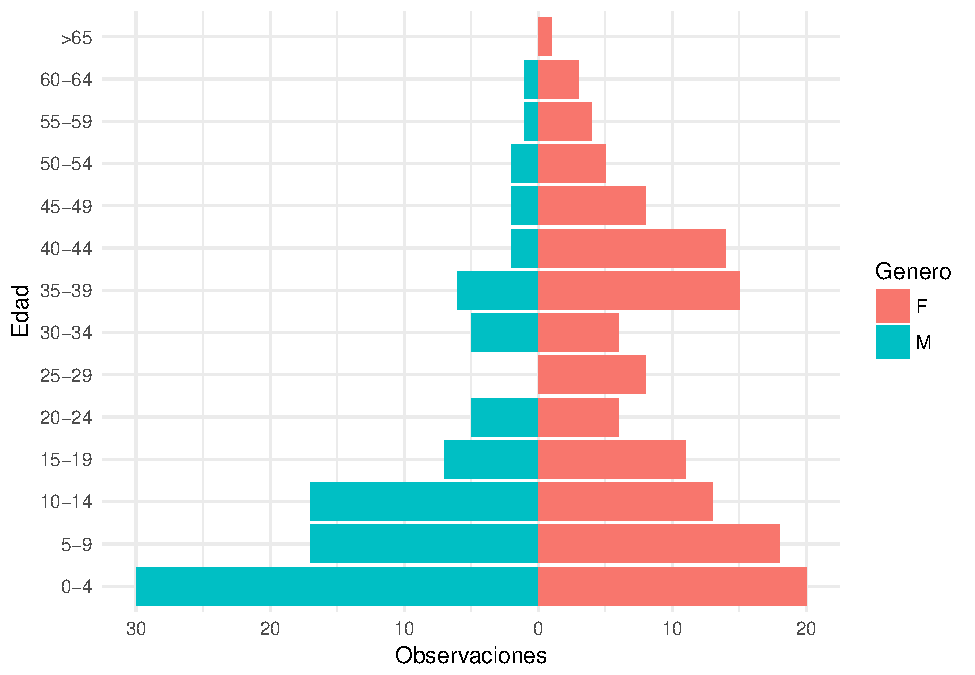
\includegraphics[width=0.5\textwidth]{Kap4/general}
	\caption{Distribución de rango de edades y géneros de los pacientes}
	\label{fig:general}
\end{figure}

\begin{figure}[H]
	\centering
	\subfigure[Distribución de variantes según su tipo.]{
		\label{f:generosgeneral}
		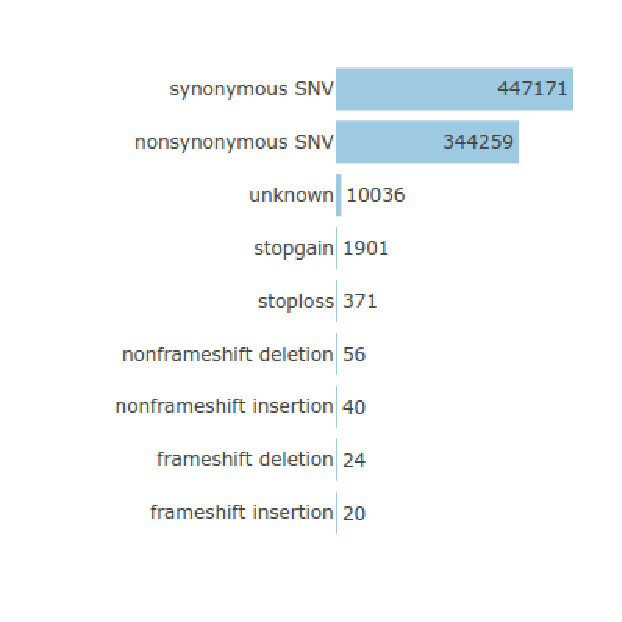
\includegraphics[width=0.35\textwidth]{Kap4/variantes.png}}
	\subfigure[Distribución de variantes por rango de edad]{
		\label{f:variantedad}
		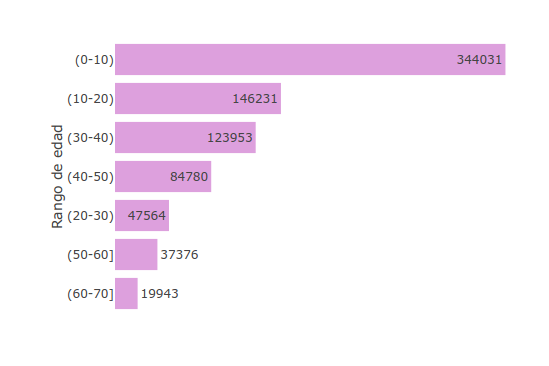
\includegraphics[width=0.55\textwidth]{Kap4/edad.png}}
	\caption{Distribución del tipo de variantes}
	\label{f:variantesgeneral}
\end{figure}

La base de datos contiene 228 pacientes de los cuales 133 son de género femenino y tienen un total de 468.485 variantes y 95 de género masculino con 345.239 de variantes obteniendo  un total de 803.878 variantes. La  figura \ref{fig:general} representa la distribución de pacientes por rango de edades y la figura \ref{f:variantesgeneral} representa la distribución de variantes según su tipo. En la figura \ref{f:generosgeneral} muestra el número de variantes que son sinónimas y no sinónimas siendo las más frecuentes en la población, a  nivel mundial se conoce que estos son lo tipos de variantes más frecuentes\cite{Fu2013}.\\

Las variantes desconocidas son el tercer tipo de variante más frecuente dado que aún existe el problema de selección del transcripto para realizar la nomenclatura adecuada de las variantes, por lo que el anotador informa que son desconocidas \cite{McCarthy2014}. La figura\ref{f:variantedad} muestra la distribución de las variantes identificadas según el rango de edad, siendo el rango con mayor número de variantes los pacientes que se encuentran entre las edades de 0 a 10 años, dado a que es la población más representada dentro de la base de datos. \\

El estado alélico de las variantes (cigocidad) que se encuentran dentro de la base de datos se dividen en heterocigotas 458639 que corresponden al 57,05\% del total de las variantes  y homocigotas 345239 que corresponden al 42,95\%. La distribución de la cigocidad de las variantes se puede explicar desde el error que se puede generar en la identificación de las variantes dado que durante el llamado  de variantes es posible que una variante homocigota se catalogue como heterocigota o si durante el proceso de secuenciación se identifican erróneamente los nucleótidos \cite{Babraham2016}\cite{Pirooznia2014}. 


\section{Análisis textual de información clínica.}

 
\subsection{Preprocesamiento.}

El proceso de limpieza y nacionalización de texto se realizo de la siguiente manera:

 \begin{enumerate}
 	\item Remoción de stop words en español, tildes y caracteres especiales como  la letra ñ y todos los documentos se unificaron en letras minúsculas.
 	\item Teniendo en cuenta la información clínica se creo un diccionario de sinónimos, donde se reemplazaron palabras que hacen referencia a una misma característica.
 	\item Calculo de la frecuencias de palabras dentro de los documentos. 
 	\item Se removieron las palabras pam,pacientes, secuenciación y gen dado que no son un factor diferenciador de los documentos.  	  
 \end{enumerate}

\subsection*{Resultados}

Los resultados que se obtuvieron para la frecuencia de palabras fueron seno, cáncer, síndrome, sospecha y años. La figura \ref{fig:sin} muestra las primeras 30 palabras más frecuentes y la nube de palabras de todos los documentos.\\

\begin{figure}[]
	\centering
	\subfigure[Nube de palabras]{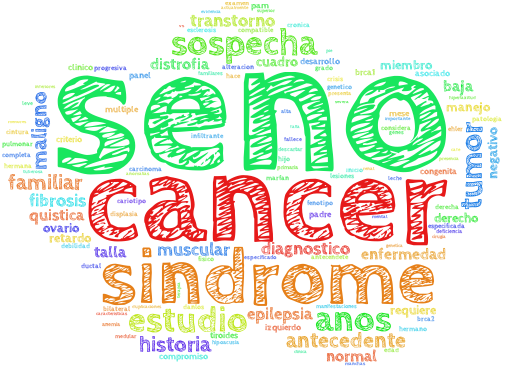
\includegraphics[width=60mm]{Kap4/sin_stop}}
	\subfigure[Frecuencia de términos]{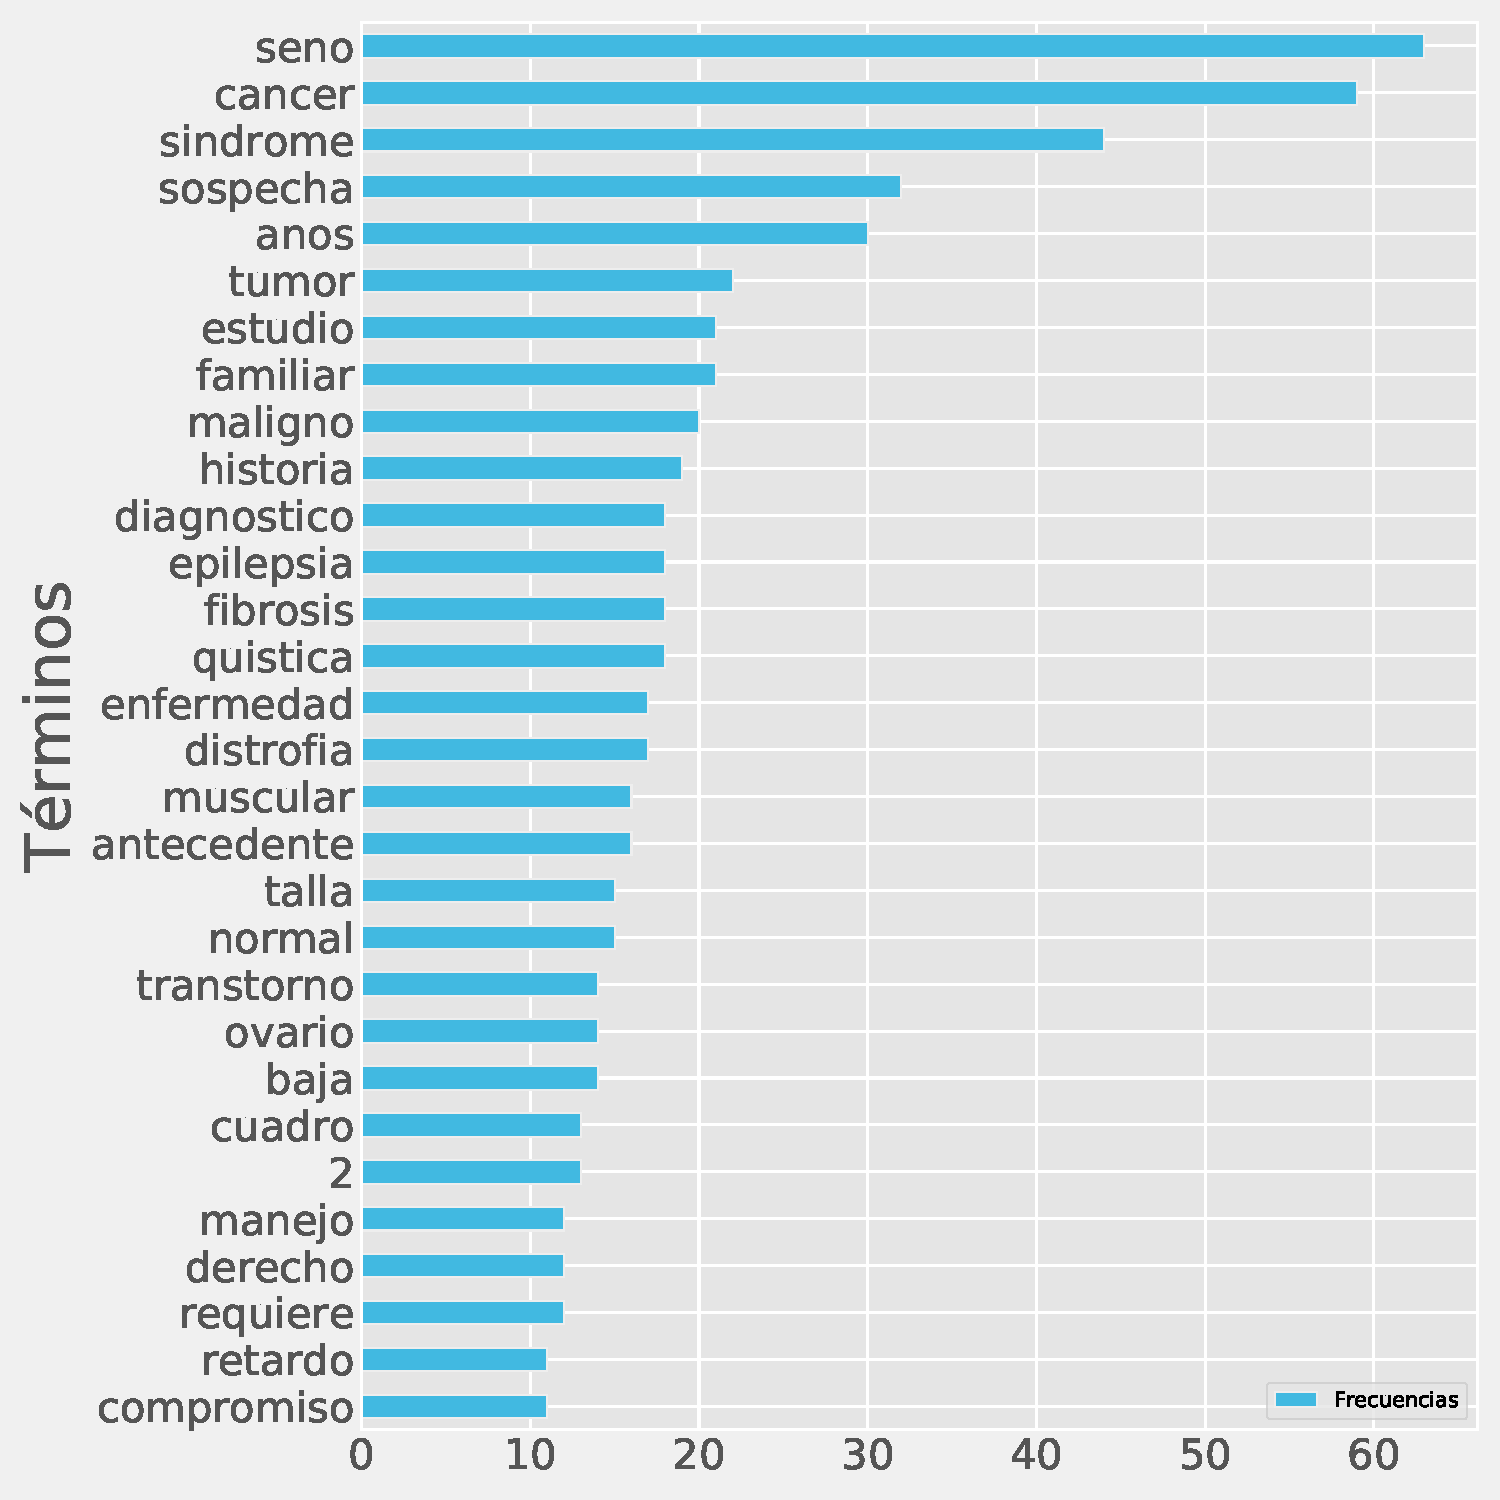
\includegraphics[width=60mm]{Kap4/frecuecias.pdf}}
	\caption{Frecuencias sin stop words y palabras sinónimas} \label{fig:sin}
\end{figure} 

Las frecuencia de palabras nos muestra las principales características de la información clínica siendo las palabras cáncer y seno los principales fenotipos, también se encuentra la palabra síndrome que puede asociarse a diferentes  enfermedades y la palabra sospecha hace referencia a diagnósticos ambiguos que pueden tener los pacientes, una de las contribuciones de la secuenciación es que basado en el fenotipo puede ayudar a un diagnóstico,entre diferentes síntomas y síndromes que pueden ser aplicados a enfermedades raras y complejas\cite{Tetreault2015a}.

\subsection{Grupos de características clínicas.}

En los procesos médicos, la relación entre los factores que pueden afectar la salud juega un papel importante. Una de las relaciones más comunes es la relación entre los genes y las enfermedades donde la secuenciación de exones tiene una alta aplicabilidad. Pero la identificación manual de este tipo de relaciones es compleja dada la cantidad de características que se pueden presentar como el diagnóstico propio de la enfermedad y/o la respuesta a los tratamientos \cite{Kawashima2017}.\\

La minería texto y puede ser aplicado al análisis en la medicina, donde el clustering (agrupamiento) puede ser considerado el método más importante que se utiliza en aprendizaje de maquina no supervisado que ha sido aplicado a diferentes problemas\cite{Kawashima2017}, teniendo en cuenta que no de los objetivos del agrupamiento de datos, es la  identificación de grupos naturales en datos sin etiquetas\cite{Jain2010}.\\

Partiendo de lo anterior el presente trabajo se implemento un modelo de agrupamiento utilizando el kmeans  para identificar grupos de características clínicas con la siguiente metodología:

\begin{enumerate}
	\item Cálculo de la matriz tf-idf y se normalizo. 
	\item Estimación de el número de k optimo.
	\item Implementación del algoritmo k-means.
	\item Validación de los clusters.
	\item Análisis de resultados. 	  
\end{enumerate}

\subsubsection{Transformación de los datos.}

El cálculo de la matriz tf-idf, se realiza a partir de frecuencia invertida con la ecuación 
$${idf}_i = \log_2 \frac{|D|}{|\{d \mid t_i \in d\}|}$$
siendo $|D|$ lo que denota el número total de documentos y donde $|\{d\mid t_i \in d\}|$ en  que $t_1$ aparece, la matriz de tf-idf es calculada a partir de la multiplicación de la frecuencia de términos y la frecuencia invertida $\mathit{tf}_{i,j} \cdot \mathit{idf}_i$ \cite{Buckley1988}. 
La figura \ref{fig:IDFTF} representa la matriz IDF-TF de las palabras que se encuentran dentro de la base de datos.  

\begin{figure}[H] 
	\centering
	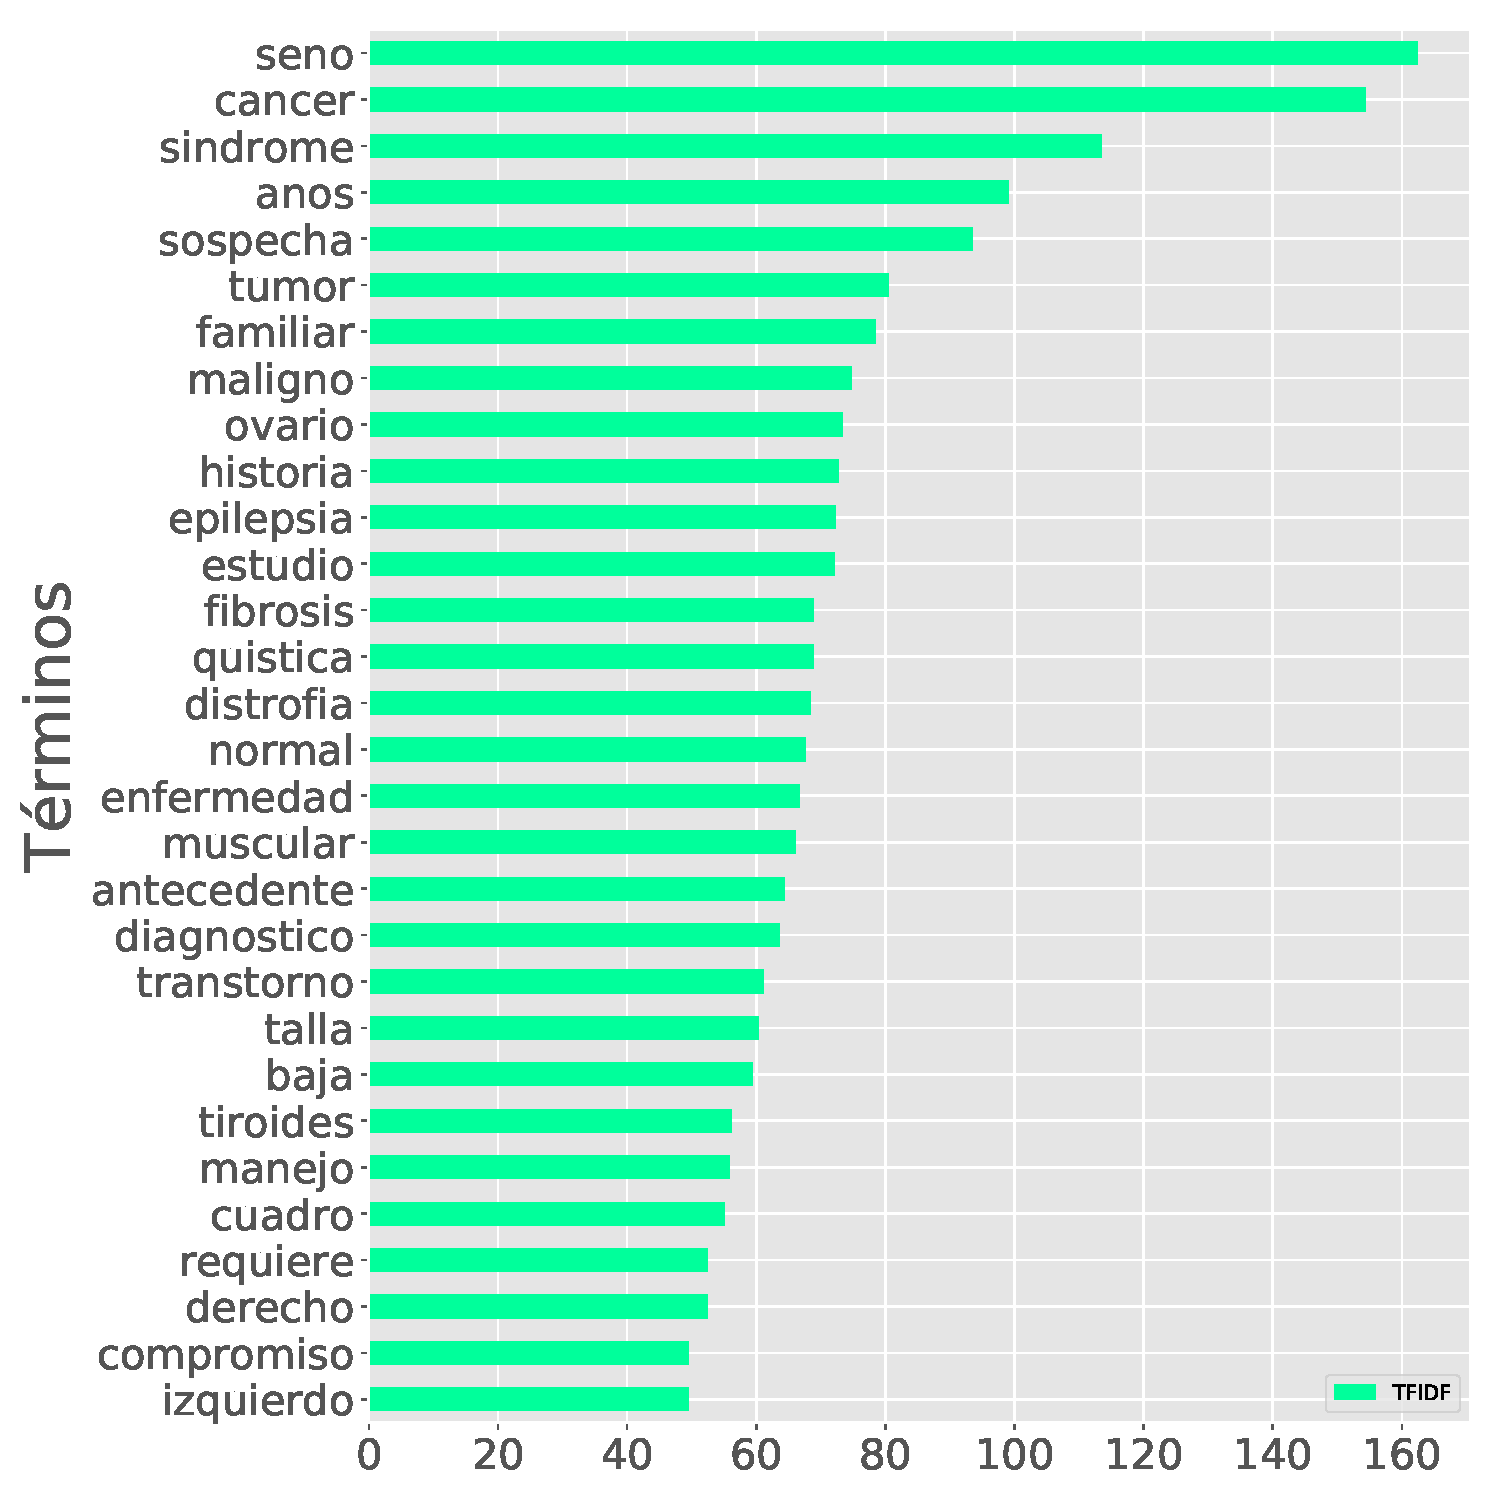
\includegraphics[width=0.5\textwidth]{Kap4/tfidf.pdf}
	\caption{TF-IDF} 
	\label{fig:IDFTF}
\end{figure}

Una vez obtenida la matriz tf-idf se normalizo y se le aplico la similaridad de coseno que es una de las medidas más populares para aplicar en documentos de texto. Esta medida tiene como ventaja que es independiente del largo del documento \cite{Huang2008}.Esta similitud fue computada de acuerdo a la siguiente formula donde la similitud ente $u$  y $v$ es definida como  según la librería scipy de python \cite{scipy}, Donde posteriormente los datos fueron utilizados para el clustering:
$$   1 - \frac{u \cdot v}
{||u||_2 ||v||_2}. $$

donde $u.v$ donde el punto es el producto de $u$ y $v$.

\subsubsection{Validación del modelo de clustering.}

La selección del número óptimo de $K$ se realizo utilizando el método del codo, este es uno de los métodos más antiguos para determinar el número de de cluster, se realizan varios experimentos iniciando por un $K$ = 2 y realizando un incremento de 1, para los cuáles se calcula el costo que conlleva cada una de las ejecuciones; entre más se aumente el número de $K7$ el costo disminuye y el número de $K$ alcanza una meseta, este valor es el que se desea obtener, visualmente se realiza la identificación mediente un gráfico de error cuadrático y número de clusters , la razón es que al continuar el aumento del número de K los nuevos clusters son muy cercanos a otros ya generados \cite{Kodinariya2013}.\\   

El cálculo del error cuadrático vs el número de clusters se realizo utilizando la libreria de python scikit learn, donde se computa el valor de la inercia que es calculada como la suma de cuadrados por cada punto cercano al centroide y es asignado al cluster. Así que  $I = \sum_{i}(d(i,cr))$ donde $cr$ es el centroide que fue asignado al cluster y $d$ es la distancia cuadrada \cite{scikit-learn}. 

\begin{figure}[H] 
	\centering
	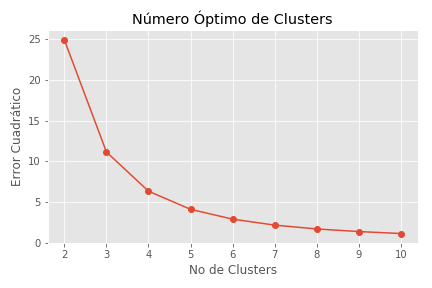
\includegraphics[width=0.5\textwidth]{Kap4/Clusters}
	\caption{Número optimo de clusters} 
	\label{fig:Clusters}
\end{figure}

Una vez se computo la inercia se realizo genero el gráfico del error cuadrático vs el número de clusters  la figura \ref{fig:Clusters} muestra el gráfico de codo obtenido, donde se puede seleccionar el cluster 5 y 6 como óptimo de $K$.\\

Para definir el número de optimo de $K$ también se computo el coeficiente de Silhouette que es una evaluación de los clusters, donde los valores altos son relacionados a modelos que tienen clusteres bien definidos .El coefiente está definido por cada muestra y está compuesta por dos valores que son \cite{scikit-learn,Rousseeuw1987}:

\begin{itemize}
	\item \textbf{a:} La distancia media entre una muestra y todos los puntos de la misma clase.
	\item \textbf{b:} La distancia media entre una muestra y todos los otros puntos en el próximo cluster más cercano.
\end{itemize}

El coeficiente Silhouette $s$ para una sola muestra se da como:

$$s = \frac{b-a}{max(a,b)}$$

Para un set de datos el coeficiente Silhouette es el promedio del coeficiente por cada muestra \cite{scikit-learn,Rousseeuw1987}. En el presente trabajo los resultados del coeficiente de Silhouette fue de  \textit{0.534}, adicionalmente se gráfico los valores de del coeficiente Silhouette para un $K$ = 5 y se presenta en la figura \ref{fig:S}:

\begin{figure}[H] 
	\centering
	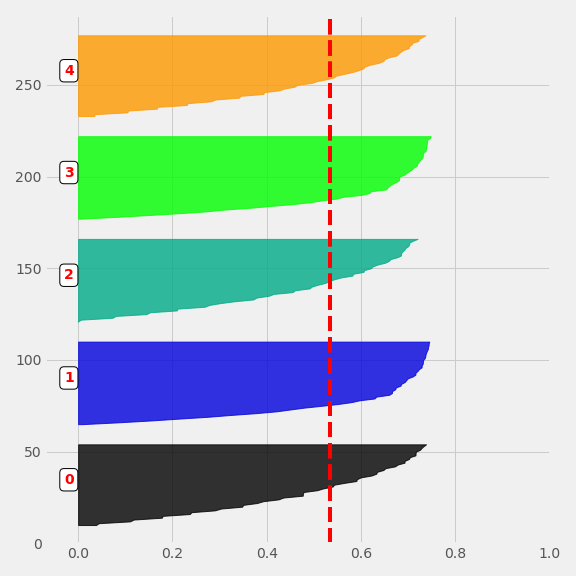
\includegraphics[width=0.3\textwidth]{Kap4/S}
	\caption{Valor Silhouette por cada cluster} 
	\label{fig:S}
\end{figure}

Para los clusters obtenidos se calcularon las medidas de validación que están dentro de la librería scikit-learn \cite{scikit-learn} son:

\begin{itemize}
	\item  \textbf{Homogeneidad:} Definida como donde cada cluster contiene solo datos de una misma clase.
	\item \textbf{Integridad:} Donde todos los miembros de una misma clase son asignados al mismo clúster.	
	\item \textbf{V-measure:} Es la medida armónica ente la homogeneidad y la integridad \cite{Rosenberg2007}. 		
\end{itemize}

El cálculo de la homogeneidad y la integridad del cluster es realizada por:
$$h=1- \frac{H(C|K)}{H(C)} $$

$$c=1- \frac{H(K|C)}{H(K)}$$

donde $H(C|K)$ es la entropía condicional de las clases en cada asignación de cluster y que son calculadas por:

$$H(C|K)= - \sum_{c=1}^{|C|} \sum_{k=1}^{|K|} \frac{n_c,_k}{n} . \log \frac{n_c,_k}{n_k}$$ 

y $H(C)$ es la entropia de clases y es calculada:
$$H(C)=  - \sum_{c=1}^{|C|} \frac{n_c}{n} . \log \frac{n_c}{n}$$ 
con $n$ que es el número total de muestras $n_c$ y $n_k$ son el número de muestras asignadas respectivamente a la clase $c$ y al cluster $k$, y finalmente $n_c,_k$ son el número de muestras de las clases$c$ asignadas al cluster $k$.

Finalmente el V-measure está definido de la siguiente manera \cite{Rosenberg2007}:

$$v= 2.\frac{h.c}{h+c}$$

También se calculo Rand-Index que calcula una medida de similitud entre dos grupos al cosiderar todos los pares de las muestras y los pares de conteo que se asignan al mismo cluster o en diferentes grupos. Calculado de la siguente manera \cite{scikit-learn}:
$$ARI = (RI - Expected_RI) / (max(RI) - Expected_RI)$$

Los resultados de validación obtenidos fueron:

Para homogeneidad 0.296, para integridad 1.0, para el V-measure 0.457 y el Rand-Index fue 0. La homogeneidad perfecta sería con un valor de 1.0, en los presentes clusters presentan una baja homogeneidad, pero una una integridad de 1.0 que significa que las etiquetas son perfectamente completas, esto se ve reflejado en el V-measure que es de 0.457 donde tenemos clusters con baja homogeneidad pero una alta integridad.  Rand-Index se obtuvo un valor de 0.0 que muestra que las clases están separadas en diferentes clusters \cite{scikit-learn}. 

\section{Asociación de grupos con variantes.}

Una vez realizado el agrupamiento de la información clínica se aplico un modelo de asociación de las variantes con los clusters obtenidos de la siguiente forma:

\begin{enumerate}
	\item Consulta de las variantes que se encontraban en cada cluster.
	\item Asociación de las variantes por cluster.
	\item Asociación de las variantes por toda la información de la base de datos filtrada por el gen CFTR como caso de ejemplo.
\end{enumerate}

La minería de datos frecuentes y las reglas de asociación  es un método popular y bien investigado par describir las relaciones entre variantes en grandes bases de datos \cite{Hahsler2005}. Las reglas de asociación (RA) muestran atributos con valores que ocurren frecuentemente en el set de datos, es posible obtener todos las posibles reglas de algunos atributos de acuerdo a la presencia de otros atributos \cite{Karabatak2009}.\\

Las reglas de asociación se basan en un set de items(elementos) $I = \{i_1,i_2,.....i_n \}$ que son un conjunto de $n$ atributos binarios. También se tiene que $D = \{t_1,t_2,..... t_m\}$ son el número de transacciones en la base de datos, cada transacción $D$ tiene una identificación única y contienen un subconjunto de elementos en $I$. Una regla se define como una implicación de la forma $X \Rightarrow Y$ donde $X,Y \subseteq I$ y $X \bigcap Y = \emptyset$. Los sets de elementos son llamados $antecedentes$ y $consecuentes$ \cite{Hahsler2005,Karabatak2009}.La selección de reglas interesantes se realiza calculando la confianza y el soporte que son definidos como:

\begin{itemize}
	\item Dados un set de datos $X \Rightarrow Y$, en una \textit{regla de asociación} tiene una confianza $c$ si $c$ de nuestra transacción que contiene $X$ pero que también contiene $Y$ \cite{Agrawal1994}.
	
	\item Dados un set de datos $X \Rightarrow Y$ tiene una \textit{regla de asociación} tiene un soporte $s$ si $s\%$ de las transacciones en nuestra base de datos de transacciones que contienen $X\cup Y$ \cite{Agrawal1994}. 
	
	\item Los algoritmos de asociación tratan de encontrar todas las reglas que tengan un mínimo de soporte y un mínimo de confianza\cite{Agrawal1994}. 

\end{itemize}

\subsection{Variantes vistas como transacciones.}

Uno de los criterios más importantes para la clasificación de variantes es la frecuencia con la que se presentan las variantes dentro de una población según la asociación americana de genética médica \cite{Laboratories2015}, otro de los retos de los análisis de variantes es el estado alélico de las variantes, que se define como una forma alternativa de un mismo gen, en este caso se aplica a las variantes encontradas dentro de la secuenciación.\\

Este estado alelico puede ser de tres tipos, el homocigoto donde el individo presenta la misma una sola variante y la otra es normal (en términos al genoma de referencia), la otra forma son los heterocigotos, donde solo una variante es distinta con respecto a su referencia y los heterocigotos compuestos que son variantes heterocigotas pero que pueden estar dentro del mismo gen o asociadas con otros. Teniendo en cuenta lo anterior es importante visualizar el estado alélico de las variantes \cite{Laboratories2015.Hannah-Shmouni2015} ya que pueden tener un impacto el el fenotipo del paciente.La realización de identificación entre la relación genotipo-fenotipo,  se ingresan como los patrones de frecuencia de las variantes y que para el trabajo caso serían las transacciones\cite{Breuer2017}.  

\subsection{Experimentación}

La confianza y el soporte para este trabajo se ajusto a partir de los resultados experimentales, donde se observo que el soporte es inversamente proporcional a la confianza, esto se debe a la cantidad de variantes que se encuentran dentro de la base de datos. Al correr un experimento con un soporte de 0.2 y una confianza de 0.9 no se generaban ningún tipo de regla, por lo tanto se fue disminuyendo en 0.1 el valor de la confianza y el soporte, finalmente se ajusto un soporte de 0.05 y una confianza de 0.6, dado que con un soporte de 0.1 solo se generaban 5 reglas, utilizando toda los datos disponibles. Una vez realizado este ajuste se dejaron los valores de soporte y confianza igual para todos los experimentos.\\

Un vez se obtuvieron los clusters de la base de datos, se realizaron 12 experimentos, los primeros 5 experimentos con todas las variante dentro del set de datos  junto a su clusters, otro a todo el conjunto de datos aplicado con  los datos y filtrado por el gen CFTR. Se volvieron a repetir los mismos experimentos pero removiendo las variantes sinónimas que son las más frecuentes dentro del conjunto de datos.


\subsubsection{Resultados} 

Teniendo en cuenta las medidas de validación encontramos  5 clusters con las siguientes estructuras:

\subsubsection*{Cluster 1}

\begin{figure}[H]
	\centering
	\subfigure[Nube de palabras]{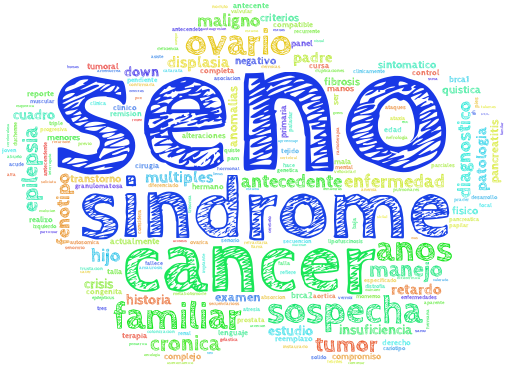
\includegraphics[width=70mm]{Kap4/cluster1}}
	\label{f:nube1}
	\subfigure[Distribucón demográfica de los pacientes]{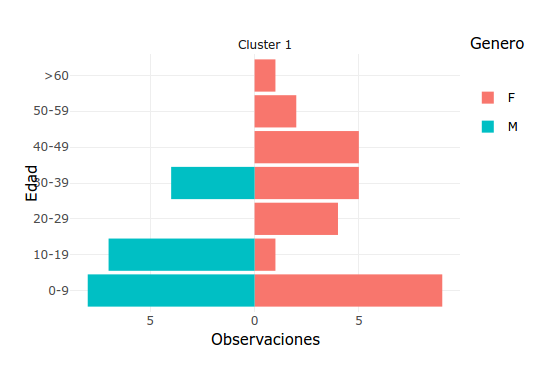
\includegraphics[width=70mm]{Kap4/edadc1}}
	\caption{Cluster 1} \label{fig:cluster1}
\end{figure} 

La figura \ref{fig:cluster1} representa el clúster 1 con la frecuencia de palabras que se agruparon para este clúster  la figura \ref{fig:cluster1}(a) se muestra la frecuencia de palabras, siendo seno,síndrome y cáncer son las palabras más frecuentes, junto con ovario,familiar sospecha y epilepsia. La figura \ref{fig:cluster1} representa la distribución de pacientes por edad y genero dentro del grupo por rango de edad en un intervalo de 10 años.\\

\begin{figure}[]
	\centering
	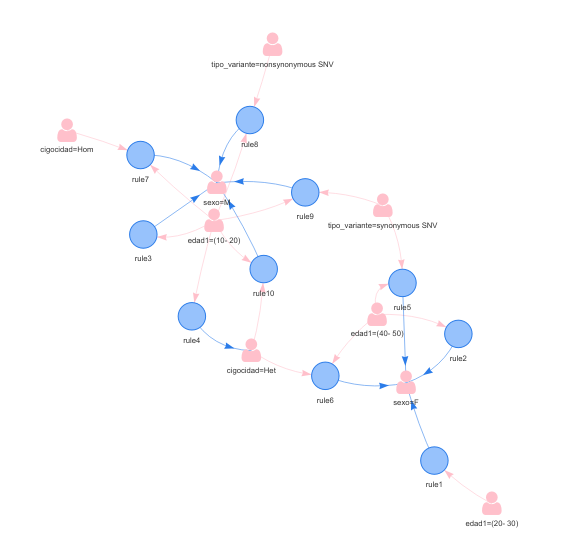
\includegraphics[width=0.5\textwidth]{Kap4/reglas1_1}
	\caption{Reglas de asociación del cluster 1 con variantes sinónimas} \label{fig:reglas1}
\end{figure}

Las primeras 10 reglas obtenidas se representan mediante la figura \ref{fig:reglas1} que muestra la asociación,sin remover las variantes sinónimas, el resultado obtenido muestra de dos tipos de variantes dentro del clúster 1. Para el genero masculino  se tiene que el tipo de variante es no sinónima, son pacientes de edad entre 10 y 20 años, el estado alélico de las variantes es homocigoto, para este grupo se observa una alta diferencia en las reglas ambos géneros.

\begin{figure}[H]
	\centering
	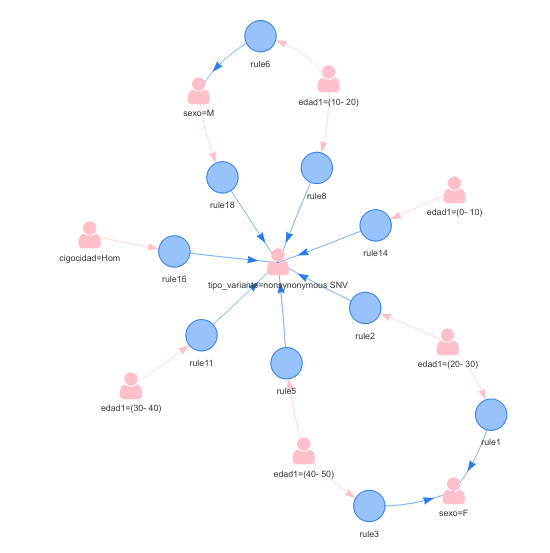
\includegraphics[width=0.5\textwidth]{Kap4/reglas1_2}
	\caption{Reglas de asociación del cluster 1 sin variantes sinónimas} \label{fig:reglas2}
\end{figure}


\subsubsection*{Cluster 2}

\begin{figure}[H]
	\centering
	\subfigure[Nube de palabras]{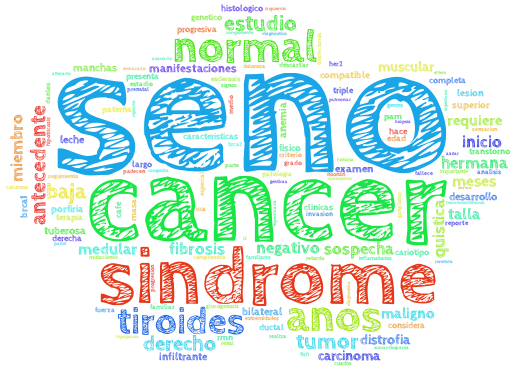
\includegraphics[width=60mm]{Kap4/cluster2}}
	\subfigure[Rango de edad en décadas.]{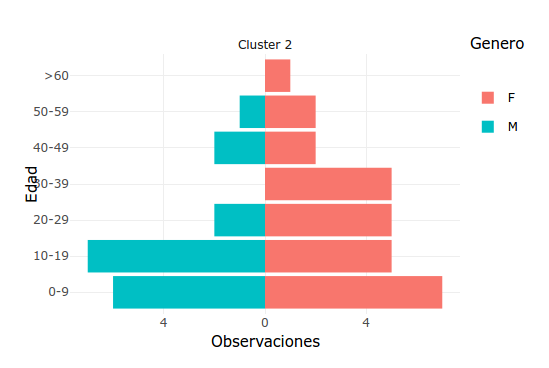
\includegraphics[width=60mm]{Kap4/edadc2}}
	\caption{Cluster 2} \label{fig:c2}
\end{figure}

\begin{figure}[H]
	\centering
	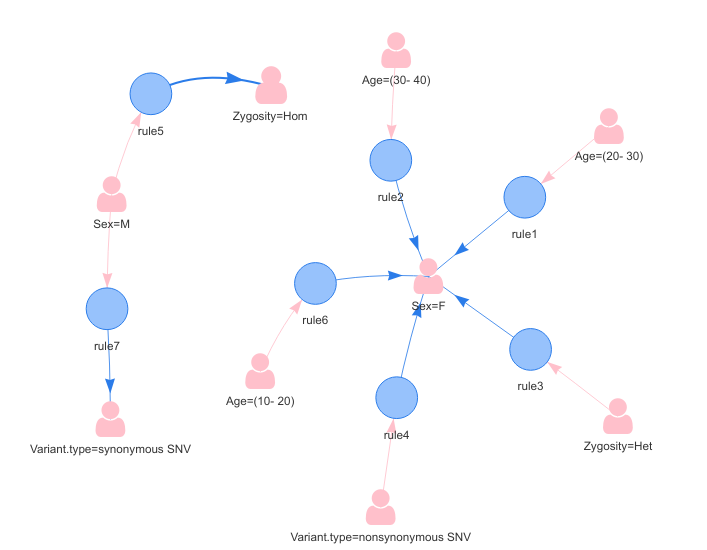
\includegraphics[width=0.5\textwidth]{Kap4/reglas2_1}
	\caption{Reglas de asociación del cluster 2 con variantes sinónimas} \label{fig:reglas2_1}
\end{figure}

\begin{figure}[H]
	\centering
	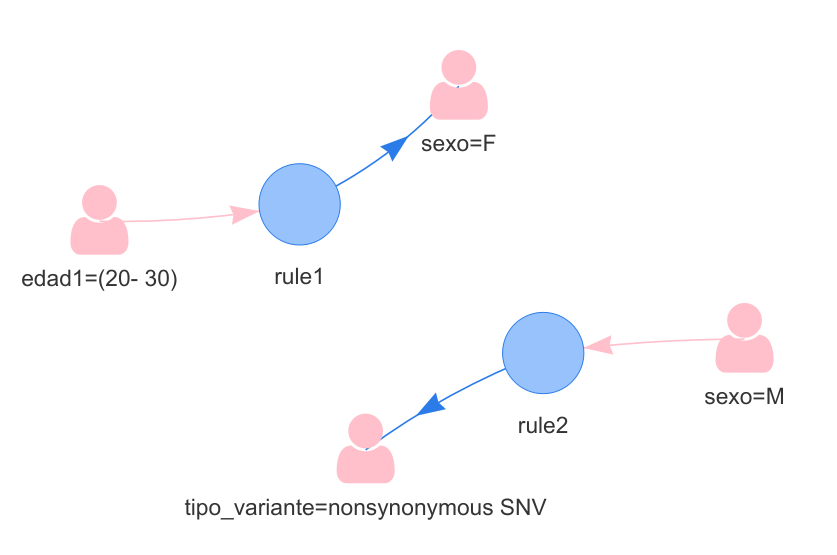
\includegraphics[width=0.5\textwidth]{Kap4/reglas2_2}
	\caption{Reglas de asociación del cluster 2 con variantes sinónimas} \label{fig:reglas2_2}
\end{figure}

\subsubsection*{Cluster 3}

\begin{figure}[H]
	\centering
	\subfigure[Nube de palabras]{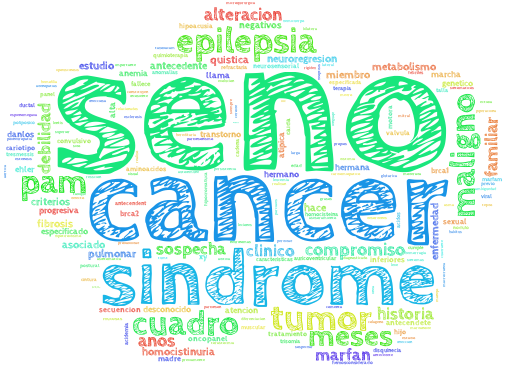
\includegraphics[width=60mm]{Kap4/cluster3}}
	\subfigure[Rango de edad en décadas.]{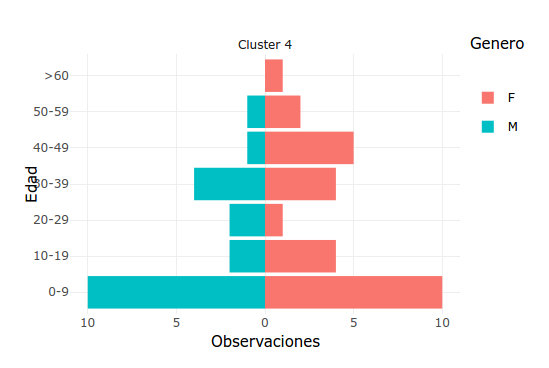
\includegraphics[width=60mm]{Kap4/edadc3}}
	\caption{Cluster 3} \label{fig:c3}
\end{figure}

\begin{figure}[H]
	\centering
	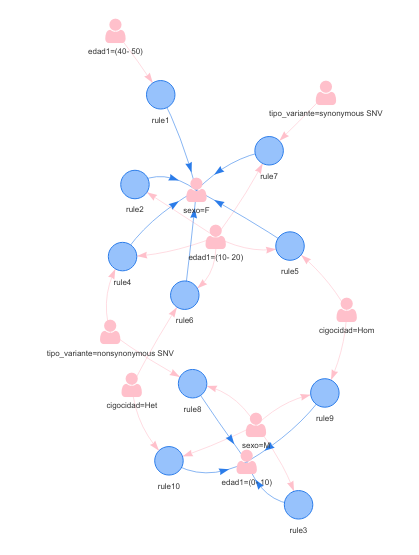
\includegraphics[width=0.5\textwidth]{Kap4/reglas3_1}
	\caption{Reglas de asociación del cluster 3 con variantes sinónimas} \label{fig:r3}
\end{figure}

\begin{figure}[H]
	\centering
	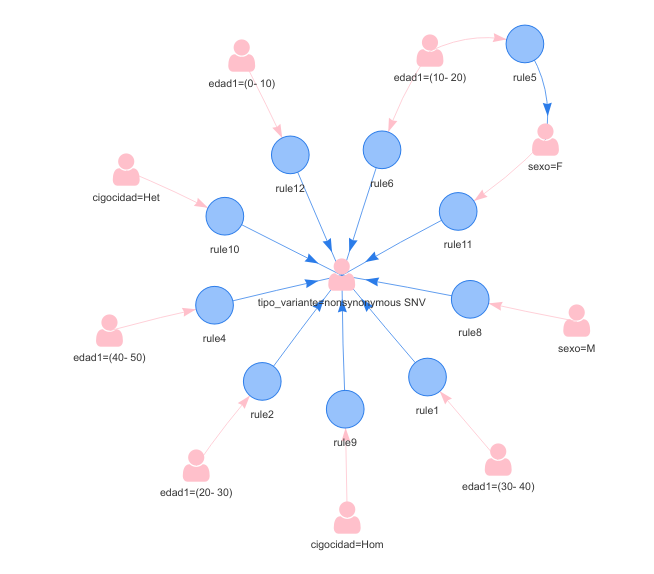
\includegraphics[width=0.5\textwidth]{Kap4/reglas3_2}
	\caption{Reglas de asociación del cluster 3 sin variantes sinónimas} \label{fig:r23}
\end{figure}

\subsubsection*{Cluster 4}
\begin{figure}[H]
	\centering
	\subfigure[Nube de palabras]{
\includegraphics[width=60mm]{Kap4/cluster4}}
	\subfigure[Rango de edad en decadas]{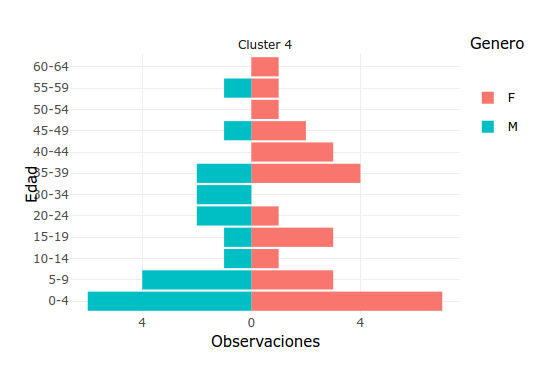
\includegraphics[width=60mm]{Kap4/edadc4}}
	\caption{Cluster 4} \label{fig:c4}
\end{figure}

\begin{figure}[H]
	\centering
	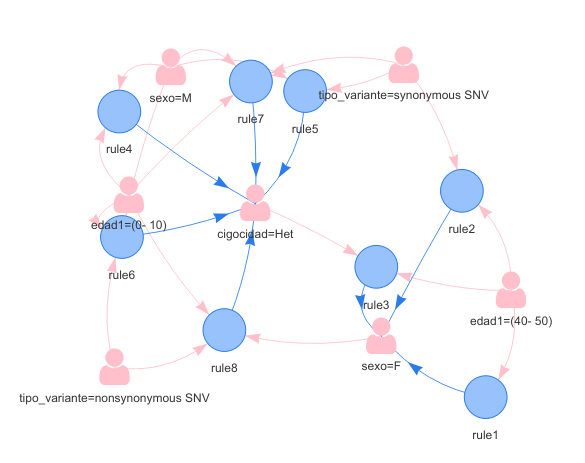
\includegraphics[width=0.5\textwidth]{Kap4/reglas4_1}
	\caption{Reglas de asociación del cluster 4 con variantes sinónimas} \label{fig:r4}
\end{figure}

\begin{figure}[H]
	\centering
	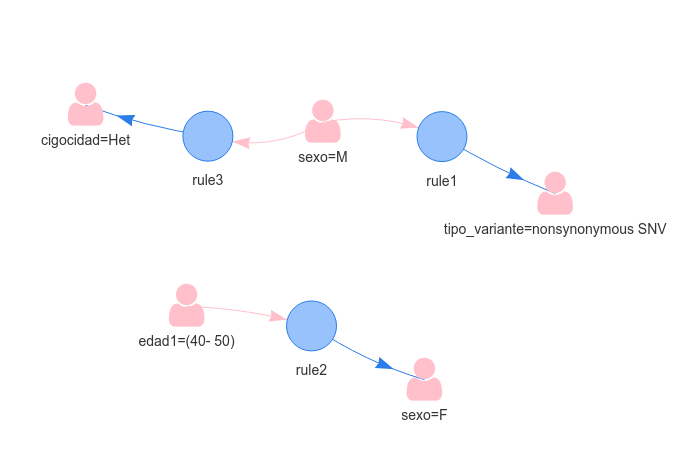
\includegraphics[width=0.5\textwidth]{Kap4/reglas4_2}
	\caption{Reglas de asociación del cluster 4 sin variantes sinónimas} \label{fig:re4}
\end{figure}

\subsubsection*{Cluster 5}

\begin{figure}[H]
	\centering
	\subfigure[Nube de palabras]{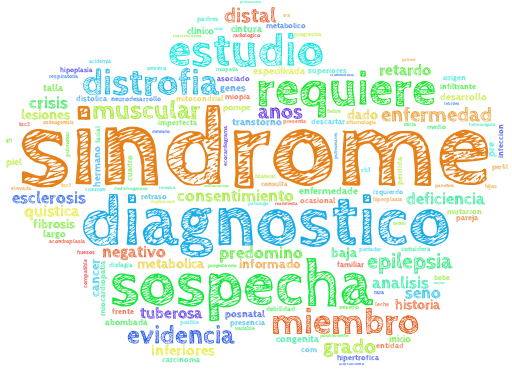
\includegraphics[width=60mm]{Kap4/cluster5}}
	\subfigure[Rango de edad en decadas]{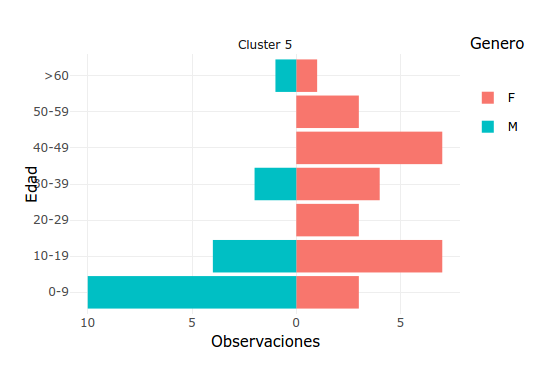
\includegraphics[width=60mm]{Kap4/edadc5}}
	\caption{Cluster 5} \label{fig:c5}
\end{figure}

\begin{figure}[H]
	\centering
	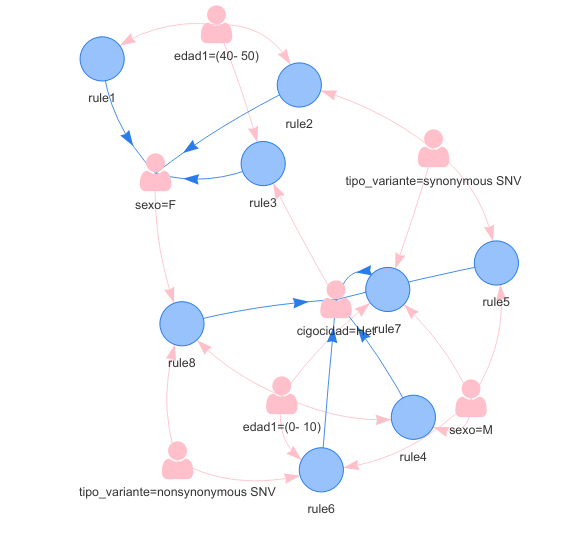
\includegraphics[width=0.5\textwidth]{Kap4/reglas5_1}
	\caption{Reglas de asociación del cluster 5 con variantes sinónimas} \label{fig:r5}
\end{figure}

\begin{figure}[H]
	\centering
	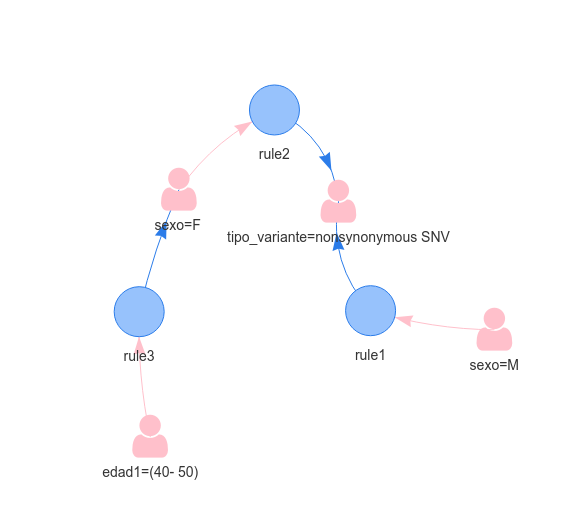
\includegraphics[width=0.5\textwidth]{Kap4/reglas5_2}
	\caption{Reglas de asociación del cluster 5 sin variantes sinónimas} \label{fig:re5}
\end{figure}

\subsubsection*{CFTR}

\begin{figure}[H]
	\centering
	\includegraphics[width=0.5\textwidth]{Kap4/CFTR1}
	\caption{Reglas de asociación con variantes sinónimas} \label{fig:r6}
\end{figure}

\begin{figure}[H]
	\centering
	\includegraphics[width=0.5\textwidth]{Kap4/CFRT2}
	\caption{Reglas de asociación sin variantes sinónimas} \label{fig:r6}
\end{figure}
\chapter{Conclusiones y trabajo futuro}

\section{Conclusiones}

\begin{itemize}
	\item La identificación de variantes es uno de los procesos más costosos de implementar a nivel comunicacional, ya que se requiere de la disponibilidad de datos si no también de conocimiento y manejo de computación de alto desempeño.
	
	\item La cantidad de herramientas para identificar variantes y la falta de concesos estándar dificultan la decisión de cuáles son las mejores herramientas y criterios para validar la identificación de variantes.
	
	\item Es necesario desarrollar herramientas que permitan hacer las ejecuciones mas rápidas y validas para identificar variantes. 
	
	\item La importancia de gestionar la información clínica y genómica dentro de un mismo sistema de información permite que se pueda almacenar por largos periodos de tiempo la información clínica,las variantes y se puedan utilizar para realizar consultas dentro de la misma. 
	
	\item La selección del gestor de la base de datos debe ser amigable, de facil manejo y que garantice la seguridad de la información ya que los datos clínicos son datos de alta sensibilidad.
	
	\item La utilización de técnicas de minería permiten realizar análisis alternativos de como es la distribución de las variantes en una población, no solo mirando el contexto del gen, si no el estado alélico de las mismas, la distribución por genero, rangos de edad y su relación con el fenotipo.
	
	\item La aplicación al gen CFTR muestra que los pacientes que tienen una sospecha de variantes patógenicas no se encuentran en regiones codificantes y que son variantes distintas a las sinónimas y no sinónimas.
	
	\item Se desarrollo una herramienta que permite la visualización de los resultados de clustering y reglas de asociación, donde se deja a disposición la utilización de los resultados para generar nuevas preguntas.
	
	\item Se presenta una de las primeras base de datos con información de variantes en la población colombiana a nivel de regiones codificantes.
	 
\end{itemize}

\subsection{Trabajo futuro}

Propuestas de futuras investigaciones:

\begin{itemize}
	\item[$\Rightarrow$] Aumentar el número de pacientes secuenciados, con el fin de aumentar la búsqueda de patrones de variantes en la población colombiana.
	
	\item[$\Rightarrow$] Aplicar el mismo modelo de minería utilizando variantes de exomas  y genomas completos para aumentar la cantidad de variantes y su tipo, además de relacionar las variantes intrónicas e intergenicas como posibles variantes causales de enfermedades teniendo en cuenta también el fenotipo de los pacientes.
	
	\item[$\Rightarrow$] Integrar información de origen regional de los pacientes, para observar la distribución de variantes  y las enfermedades por regiones en Colombia.
	
	\item[$\Rightarrow$] Desarrollar una base de datos NoSQL para integrar la información de variantes proveniente de diversos anotadores, con frecuencias poblacionales y con predicotres de patogenicidad de la variantes y la información clínica, además de dejar abierta la posibilidad de agregar más columnas con nueva información de interés haciéndola la base de datos mas permeable a los cambios que hagan las herramientas de anotación. 

\end{itemize}

\chapter{Conclusiones y recomendaciones}
\section{Conclusiones}
Las conclusiones constituyen un cap\'{\i}tulo independiente y presentan, en forma l\'{o}gica, los resultados de la tesis  o trabajo de investigaci\'{o}n. Las conclusiones deben ser la respuesta a los objetivos o prop\'{o}sitos planteados. Se deben titular con la palabra conclusiones en el mismo formato de los t\'{\i}tulos de los cap\'{\i}tulos anteriores (T\'{\i}tulos primer nivel), precedida por el numeral correspondiente (seg\'{u}n la presente plantilla).\\

\section{Recomendaciones}
Se presentan como una serie de aspectos que se podr\'{\i}an realizar en un futuro para emprender investigaciones similares o fortalecer la investigaci\'{o}n realizada. Deben contemplar las perspectivas de la investigaci\'{o}n, las cuales son sugerencias, proyecciones o alternativas que se presentan para modificar, cambiar o incidir sobre una situaci\'{o}n espec\'{\i}fica o una problem\'{a}tica encontrada. Pueden presentarse como un texto con caracter\'{\i}sticas argumentativas, resultado de una reflexi\'{o}n acerca de la tesis o trabajo de investigaci\'{o}n.\\
\begin{appendix}
\chapter{Anexo: Nombrar el anexo A de acuerdo con su contenido}\label{AnexoA}
Los Anexos son documentos o elementos que complementan el cuerpo de la tesis o trabajo de investigaci\'{o}n y que se relacionan, directa o indirectamente, con la investigaci\'{o}n, tales como acetatos, cd, normas, etc.\\

\chapter{Anexo: Nombrar el anexo B de acuerdo con su contenido}
A final del documento es opcional incluir \'{\i}ndices o glosarios. \'{E}stos son listas detalladas y especializadas de los t\'{e}rminos, nombres, autores, temas, etc., que aparecen en el mismo. Sirven para facilitar su localizaci\'{o}n en el texto. Los \'{\i}ndices pueden ser alfab\'{e}ticos, cronol\'{o}gicos, num\'{e}ricos, anal\'{\i}ticos, entre otros. Luego de cada palabra, t\'{e}rmino, etc., se pone coma y el n\'{u}mero de la p\'{a}gina donde aparece esta informaci\'{o}n.\\

\chapter{Anexo: Nombrar el anexo C de acuerdo con su contenido}
MANEJO DE LA BIBLIOGRAF\'{I}A: la bibliograf\'{\i}a es la relaci\'{o}n de las fuentes documentales consultadas por el investigador para sustentar sus trabajos. Su inclusi\'{o}n es obligatoria en todo trabajo de investigaci\'{o}n. Cada referencia bibliogr\'{a}fica se inicia contra el margen izquierdo.\\

La NTC 5613 establece los requisitos para la presentaci\'{o}n de referencias bibliogr\'{a}ficas citas y notas de pie de p\'{a}gina. Sin embargo, se tiene la libertad de usar cualquier norma bibliogr\'{a}fica de acuerdo con lo acostumbrado por cada disciplina del conocimiento. En esta medida es necesario que la norma seleccionada se aplique con rigurosidad.\\

Es necesario tener en cuenta que la norma ISO 690:1987 (en Espa\~{n}a, UNE 50-104-94) es el marco internacional que da las pautas m\'{\i}nimas para las citas bibliogr\'{a}ficas de documentos impresos y publicados. A continuaci\'{o}n se lista algunas instituciones que brindan par\'{a}metros para el manejo de las referencias bibliogr\'{a}ficas:\\

\begin{center}
\centering%
\begin{tabular}{|p {7.5 cm}|p {7.5 cm}|}\hline
\arr{Instituci\'{o}n}&Disciplina de aplicaci\'{o}n\\\hline%
Modern Language Association (MLA)&Literatura, artes y humanidades\\\hline%
American Psychological Association (APA)&Ambito de la salud (psicolog\'{\i}a, medicina) y en general en todas las ciencias sociales\\\hline
Universidad de Chicago/Turabian &Periodismo, historia y humanidades.\\\hline
AMA (Asociaci\'{o}n M\'{e}dica de los Estados Unidos)&Ambito de la salud (psicolog\'{\i}a, medicina)\\\hline
Vancouver &Todas las disciplinas\\\hline
Council of Science Editors (CSE)&En la actualidad abarca diversas ciencias\\\hline
National Library of Medicine (NLM) (Biblioteca Nacional de Medicina)&En el \'{a}mbito m\'{e}dico y, por extensi\'{o}n, en ciencias.\\\hline
Harvard System of Referencing Guide &Todas las disciplinas\\\hline
JabRef y KBibTeX &Todas las disciplinas\\\hline
\end{tabular}
\end{center}

Para incluir las referencias dentro del texto y realizar lista de la bibliograf\'{\i}a en la respectiva secci\'{o}n, puede utilizar las herramientas que Latex suministra o, revisar el instructivo desarrollado por el Sistema de Bibliotecas de la Universidad Nacional de Colombia\footnote{Ver: www.sinab.unal.edu.co}, disponible en la secci\'{o}n "Servicios", opci\'{o}n "Tr\'{a}mites" y enlace "Entrega de tesis".

\end{appendix}

\addcontentsline{toc}{chapter}{\numberline{}Bibliograf\'{\i}a}
\bibliographystyle{unsrt}
\bibliography{references}
\end{document}